\documentclass[supercite]{Experimental_Report}

\title{~~~~~~数据结构实验~~~~~~}
\author{刘欣逸}
\school{计算机科学与技术学院}
\classnum{CS2210}
\stunum{U202115473}
\instructor{郑渤龙}
\date{2023年5月29日}


\usepackage{ctex}
\usepackage{listings}
\usepackage{placeins}
\usepackage{algorithm, multirow}
\usepackage{algpseudocode}
\usepackage{amsmath}
\usepackage{amsthm}
\usepackage{framed}
\usepackage{mathtools}
\usepackage{subcaption}
\usepackage{xltxtra} %提供了针对XeTeX的改进并且加入了XeTeX的LOGO, 自动调用xunicode宏包(提供Unicode字符宏)
\usepackage{bm}
\usepackage{tikz}
\usepackage{tikzscale}
\usepackage{pgfplots}
\usepackage{enumitem}
\usepackage{fontspec}
\usepackage{xcolor}
\usepackage{listings}


\newfontfamily\sfr{SFMono-Regular}
\newfontfamily\sfb{SFMono-Bold}
\definecolor{mygreen}{rgb}{0,0.6,0}
\definecolor{mygray}{rgb}{0.5,0.5,0.5}
\definecolor{mymauve}{rgb}{0.58,0,0.82}
\lstset{ %
backgroundcolor=\color{white},   % choose the background color
basicstyle=\footnotesize\ttfamily,        % size of fonts used for the code
columns=fullflexible,
breaklines=true,                 % automatic line breaking only at whitespace
captionpos=b,                    % sets the caption-position to bottom
tabsize=4,
commentstyle=\color{mygreen},    % comment style
% escapeinside={\%*}{*)},          % if you want to add LaTeX within your code
keywordstyle=\color{blue},       % keyword style
stringstyle=\color{mymauve}\ttfamily,     % string literal style
frame=single,
rulesepcolor=\color{red!20!green!20!blue!20},
% identifierstyle=\color{red},
language=c++,
% escapechar={\"*\"}{(*)},
emptylines=3,
numbers=right,
numberstyle=\footnotesize\sfr,
}

% \lstset{
% 	language=C++,
% 	basicstyle=\sffamily\sfr,
% 	keywordstyle=\color{keywordColor}\sffamily\sfr,
% 	commentstyle=\color{commentColor}\sffamily\sfr,
% 	stringstyle=\color{stringColor}\sffamily\sfr,
% 	showstringspaces=false,
% 	columns=fullflexible,keepspaces,
% 	numbers=left,
% 	numberstyle=\color{numberColor}\footnotesize\sfr,
% 	escapechar=\$,
% 	morecomment=*[s][\color{stringColor}\sffamily\sfr]{<}{>},
% 	morecomment=[s][\color{characterColor}\sffamily\sfr]{'}{'},
% 	keywords=[2]{std, cout, cin},
% 	keywordstyle = [2]{\color{oglobalColor}\sffamily\sfr},
% 	keywords=[3]{endl, printf, scanf, setw, setfill, setbase, setprecision, time, ctime, rand},
% 	keywordstyle = [3]{\color{functionColor}\sffamily\sfr},
% 	keywords=[4]{\#include},
% 	keywordstyle =[4]{\color{preprocessorColor}\ssfamily\sfr},
% 	literate={
% 		{<<}{{{\color{black}<<}}}1
% 		{>>}{{{\color{black}>>}}}1
% 		{*}{{{*}}}1
% 		{0}{{{\color{characterColor}0}}}1
% 		{1}{{{\color{characterColor}1}}}1
% 		{2}{{{\color{characterColor}2}}}1
% 		{3}{{{\color{characterColor}3}}}1
% 		{4}{{{\color{characterColor}4}}}1
% 		{5}{{{\color{characterColor}5}}}1
% 		{6}{{{\color{characterColor}6}}}1
% 		{7}{{{\color{characterColor}7}}}1
% 		{8}{{{\color{characterColor}8}}}1
% 		{9}{{{\color{characterColor}9}}}1
% 		},
% 	tabsize=4,
% 	frame=single,
% 	frameround=tttt
% }


\pgfplotsset{compat=1.16}

\newcommand{\cfig}[3]{
  \begin{figure}[htb]
    \centering
    \includegraphics[width=#2\textwidth]{images/#1.tikz}
    \caption{#3}
    \label{fig:#1}
  \end{figure}
}

\newcommand{\sfig}[3]{
  \begin{subfigure}[b]{#2\textwidth}
    \includegraphics[width=\textwidth]{images/#1.tikz}
    \caption{#3}
    \label{fig:#1}
  \end{subfigure}
}

\newcommand{\xfig}[3]{
  \begin{figure}[htb]
    \centering
    #3
    \caption{#2}
    \label{fig:#1}
  \end{figure}
}

\newcommand{\rfig}[1]{\autoref{fig:#1}}
\newcommand{\ralg}[1]{\autoref{alg:#1}}
\newcommand{\rthm}[1]{\autoref{thm:#1}}
\newcommand{\rlem}[1]{\autoref{lem:#1}}
\newcommand{\reqn}[1]{\autoref{eqn:#1}}
\newcommand{\rtbl}[1]{\autoref{tbl:#1}}

\algnewcommand\Null{\textsc{null }}
\algnewcommand\algorithmicinput{\textbf{Input:}}
\algnewcommand\Input{\item[\algorithmicinput]}
\algnewcommand\algorithmicoutput{\textbf{Output:}}
\algnewcommand\Output{\item[\algorithmicoutput]}
\algnewcommand\algorithmicbreak{\textbf{break}}
\algnewcommand\Break{\algorithmicbreak}
\algnewcommand\algorithmiccontinue{\textbf{continue}}
\algnewcommand\Continue{\algorithmiccontinue}
\algnewcommand{\LeftCom}[1]{\State $\triangleright$ #1}

\newtheorem{thm}{定理}[section]
\newtheorem{lem}{引理}[section]

\colorlet{shadecolor}{black!15}

\theoremstyle{definition}
\newtheorem{alg}{算法}[section]

\def\thmautorefname~#1\null{定理~#1~\null}
\def\lemautorefname~#1\null{引理~#1~\null}
\def\algautorefname~#1\null{算法~#1~\null}

\begin{document}

\maketitle

\clearpage

\pagenumbering{Roman}

\tableofcontents[level=2]

\clearpage

\pagenumbering{arabic}

\section{基于顺序存储结构的线性表实现}


\subsection{问题描述}


要求构造一个具有菜单的功能演示系统。该演示系统实现多个线性表管理。其中,在主函数中准备函数调用所需实参值、显示函数执行结果,并给出适当的操作提示。

实现依据最小完备性和常用性相结合的原则确定的初始化表、销毁表、清空表、判定空表、求表长和获得元素等12种基本运算,具体运算功能定义如下。
\begin{enumerate}
	\item 初始化表:函数名称是\verb|InitaList(L)|;初始条件是线性表\verb|L|不存在已存在;操作结果是构造一个空的线性表。
	\item 销毁表:函数名称是\verb|DestroyList(L)|;初始条件是线性表\verb|L|已存在;操作结果是销毁线性表\verb|L|。
	\item 清空表:函数名称是\verb|ClearList(L)|;初始条件是线性表\verb|L|已存在;操作结果是将\verb|L|重置为空表。
	\item 判定空表:函数名称是\verb|ListEmpty(L)|;初始条件是线性表\verb|L|已存在;操作结果是若\verb|L|为空表则返回\verb|TRUE|,否则返回\verb|FALSE|。
	\item 求表长:函数名称是\verb|ListLength(L)|;初始条件是线性表\verb|L|已存在;操作结果是返回\verb|L|中数据元素的个数。
	\item 获得元素:函数名称是\verb|GetElem(L,i,e)|;初始条件是线性表\verb|L|已存在, \\ \verb|1<=i<=ListLength(L)|;操作结果是用\verb|e|返回\verb|L|中第\verb|i|个数据元素的值。
	\item 查找元素:函数名称是\verb|LocateElem(L,e,compare())|;初始条件是线性表\verb|L|已存在;操作结果是返回\verb|L|中第一个与\verb|e|满足关系\verb|compare()|关系的数据元素的位序,若这样的数据元素不存在,则返回值为\verb|0|。
	\item 获得前驱:函数名称是\verb|PriorElem(L,cur_e,pre_e)|;初始条件是线性表\verb|L|已存在;操作结果是若\verb|cur_e|是\verb|L|的数据元素,且不是第一个,则用\verb|pre_e|返回它的前驱,否则操作失败,\verb|pre_e|无定义。
	\item 获得后继:函数名称是\verb|NextElem(L,cur_e,next_e)|;初始条件是线性表\verb|L|已存在;操作结果是若\verb|cur_e|是\verb|L|的数据元素,且不是最后一个,则用\verb|next_e|返回它的后继,否则操作失败,\verb|next_e|无定义。
	\item 插入元素:函数名称是\verb|ListInsert(L,i,e)|;初始条件是线性表\verb|L|已存在,\\ \verb|1<=i<=ListLength(L)+1|;操作结果是在\verb|L|的第\verb|i|个位置之前插入新的数据元素\verb|e|。
	\item 删除元素:函数名称是\verb|ListDelete(L,i,e)|;初始条件是线性表\verb|L|已存在且非空,\verb|1<=i<=ListLength(L)|;操作结果:删除\verb|L|的第\verb|i|个数据元素,用\verb|e|返回其值。
	\item 遍历表:函数名称是\verb|ListTraverse(L,visit())|,初始条件是线性表\verb|L|已存在;操作结果是依次对\verb|L|的每个数据元素调用函数\verb|visit()|。
\end{enumerate}
此外,还在基础功能的基础上实现了附加功能:
\begin{enumerate}
	\item 最大连续子数组和:函数名称是\verb|MaxSubArray(L)|;初始条件是线性表\verb|L|已存在且非空,请找出一个具有最大和的连续子数组(子数组最少包含一个元素),操作结果是其最大和;
	\item 和为\verb|K|的子数组:函数名称是\verb|SubArrayNum(L,k)|; 初始条件是线性表\verb|L|已存在且非空,操作结果是该数组中和为\verb|k|的连续子数组的个数;
	\item 顺序表排序:函数名称是\verb|SortList(L)|;初始条件是线性表\verb|L|已存在;操作结果是将\verb|L|由小到大排序;
	\item 实现线性表的文件形式保存:其中,
	\begin{itemize}
		\item 需要设计文件数据记录格式,以高效保存线性表数据逻辑结构\verb|(D,{R})|的完整信息;
		\item  需要设计线性表文件保存和加载操作合理模式。
	\end{itemize}
	\item 实现多个线性表管理:设计相应的数据结构管理多个线性表的查找、添加、移除等功能。
\end{enumerate}
实验目的:
\begin{enumerate}
	\item 加深对线性表的概念、基本运算的理解;
	\item 熟练掌握线性表的逻辑结构与物理结构的关系;
	\item 物理结构采用顺序表,熟练掌握线性表的基本运算的实现。
\end{enumerate}

\subsection{系统设计}
本系统提供一个采用顺序存储方式的线性表及其操作实现。
系统可供选择的操作有:
\begin{itemize}
	\item 基本操作:初始化线性表、销毁表、清空表、判定空表,求表长、获得元素、查找元素、获得某元素的前驱、获得某元素的后继、插入元素、删除元素、遍历线性表。
	\item 附加功能:最大连续子数组和、和为\verb|K|的子数组、顺序表排序、实现线性表的文件形式保存、实现多个线性表管理。
\end{itemize}

\subsubsection{头文件、宏和类型定义}
\begin{lstlisting}
#include <stdio.h>
#include <stdlib.h>
#include <string.h>
#include <limits.h>

#define TRUE 1
#define FALSE 0
#define OK 1
#define ERROR 0
#define INFEASIBLE -1
#define OVERFLOW -2
#define ISEMPTY -3
#define LIST_INIT_SIZE 1000
#define LISTINCREMENT  10
#define max(i,j) ((i)>(j)?(i):(j))

typedef int status;
typedef int ElemType; // 数据元素类型定义
typedef struct{  // 顺序表(顺序结构)的定义
    ElemType * elem;
    int length;
    int listsize;
} SqList;

typedef struct THELISTS{  // 顺序表的管理表定义
	 struct ALIST{
		 char name[30];
		 SqList L;
	  } elem[50];
	  int length = 0;
	  int listssize = 50;
 } LISTS;
\end{lstlisting}

\subsubsection{函数设计}
\begin{enumerate}
\item 函数名称:\verb|InitaList(L)|;

初始条件:线性表\verb|L|不存在;

操作结果:是构造一个空的线性表;

设计思路:先分配存储空间后,将表长设为\verb|0|,再将线性表容量变量设为预定义的初始存储容量。

\item 函数名称:\verb|DestroyList(L)|;

初始条件:线性表\verb|L|已存在;

操作结果:销毁线性表\verb|L|;

设计思路:释放内存并将其他结构成员设置为初值。

\item 函数名称:\verb|ClearList(L)|;

初始条件:线性表\verb|L|已存在;

操作结果:将\verb|L|重置为空表;

设计思路:将表长设为\verb|0|。

\item 函数名称:\verb|ListEmpty(L)|;

初始条件:线性表\verb|L|已存在;

操作结果:若\verb|L|为空表则返回\verb|TRUE|,否则返回\verb|FALSE|;

设计思路:表长为\verb|0|则为空表,否则不是空。

\item 函数名称:\verb|ListLength(L)|;

初始条件:线性表\verb|L|已存在;

操作结果:返回\verb|L|中数据元素的个数;

设计思路:返回线性表表长的值。

\item 函数名称:\verb|GetElem(L,i,e)|;

初始条件:线性表已存在,\verb|1<=i<=ListLength(L)|;

操作结果:用\verb|e|返回\verb|L|中第\verb|i|个数据元素的值;

设计思路:将线性表中第\verb|i|个数据元素的值赋值给\verb|e|。

\item 函数名称:\verb|LocateElem(L,e,compare())|;

初始条件:线性表已存在;

操作结果:返回线性表中第\verb|1|个与\verb|e|相等的数据元素的位置,若这样的数据元素不存在,则返回值为\verb|0|;

设计思路:从索引低位开始顺序查找,如果找到返回该元素的位序

\item 函数名称:\verb|PriorElem(L,cur_e,pre_e)|;

初始条件:线性表\verb|L|已存在;

操作结果:若\verb|cur_e|是\verb|L|的数据元素并且不是第一个数据元素,用\verb|pre_e|返回它的前驱,否则操作失败。

设计思路:首先判断该元素不是第一个数据元素,再查找该结点,如果查找成功且该结点有前驱元素,则将前驱元素赋值给\verb|pre_e|。若未找到该结点,或者该结点是第一个数据元素,则返回\verb|ERROR|。

\item 函数名称:\verb|NextElem(L,cur_e,next_e)|

初始条件:线性表\verb|L|已存在;

操作结果:若\verb|cur_e|是\verb|L|的数据元素,且不是最后一个,则用\verb|next_e|返回它的后继,否则操作失败,\verb|next_e|无定义。

设计思路:首先判断该元素不是最后一个数据元素,再查找该结点,如果查找成功且该结点有后继元素,则将后继元素赋值给\verb|next_e|。若未找到该结点,或者该结点是最后一个数据元素,则返回\verb|ERROR|。

\item 函数名称:\verb|ListInsert(L,i,e)|

初始条件:线性表\verb|L|已存在且非空,\verb|1<=i<=ListLength(L)+1|;

操作结果:在\verb|L|的第\verb|i|个位置之前插入新的数据元素\verb|e|。

设计思路:先遍历顺序表,若线性表\verb|L|已存在且不为空,输入的\verb|i|值不合法,则返回\verb|ERROR|;若\verb|i|的值合法,则在线性表的第\verb|i|个位置前插入新数据元素\verb|e|,返回\verb|OK|。若线性表\verb|L|不存在,返回\verb|INFEASIBLE|.

\item 函数名称:\verb|ListDelete(L,i,e)|;

初始条件:线性表\verb|L|已存在且非空,\verb|1<=i<=ListLength(L)|;

操作结果:删除\verb|L|的第\verb|i|个数据元素,用\verb|e|返回其值;

设计思路:先遍历顺序表,如果线性表\verb|L|已存在且非空,并且输入的\verb|i|值不合法,则返回\verb|ERROR|。若满足线性表\verb|L|已存在且\verb|L|非空,并且\verb|i|的值合法,则删除线性表的第\verb|i|个位置的数据元素,并用\verb|e|返回其值,返回\verb|OK|。

\item 函数名称:\verb|ListTraverse(L)|;

初始条件:线性表\verb|L|已存在;

操作结果:依次遍历\verb|L|的每个数据元素;

设计思路:若线性表\verb|L|存在,则依序遍历元素;否则返回\verb|ERROR|。

\item 函数名称:\verb|SaveList(L,filename)|;

初始条件:线性表\verb|L|已存在;

操作结果:将线性表\verb|L|保存到指定文件;

设计思路:用\verb|fprintf|保存为文件。

\item 函数名称:\verb|LoadList(L)|;

初始条件:文件\verb|filename|已存在;

操作结果:从文件中加载数据到\verb|L|;

设计思路:用\verb|fscanf|将文件读取顺序表。

\item 函数名称:\verb|MaxSubArray(L)|;

初始条件:线性表\verb|L|已存在;

操作结果:返回线性表\verb|L|的最大连续子数组和;

设计思路:逐个枚举子数组求出最大连续子数组和。

\item 函数名称:\verb|SubArrayNum(L,k)|;

初始条件:线性表\verb|L|已存在;

操作结果:返回线性表\verb|L|的和为k的连续子数组个数;

设计思路:逐个枚举子数组求出和为k的连续子数组个数。

\item 函数名称:\verb|SortList(L)|

初始条件:线性表\verb|L|已存在;

操作结果:将\verb|L|中的元素按升序排序;

设计思路:用冒泡排序算法将\verb|L|的数据元素按升序排序。

\end{enumerate}

\subsection{系统实现}

见《附录A 基于顺序存储结构线性表实现的源程序》。

\subsection{系统测试}
先用插入操作创建包含元素1、2、3、4、5、6、7的顺序表。再测试判空、查找、删除、遍历、销毁等基础功能。
\begin{enumerate}
\item \verb|InitList()|
	\begin{figure}[!htb]
		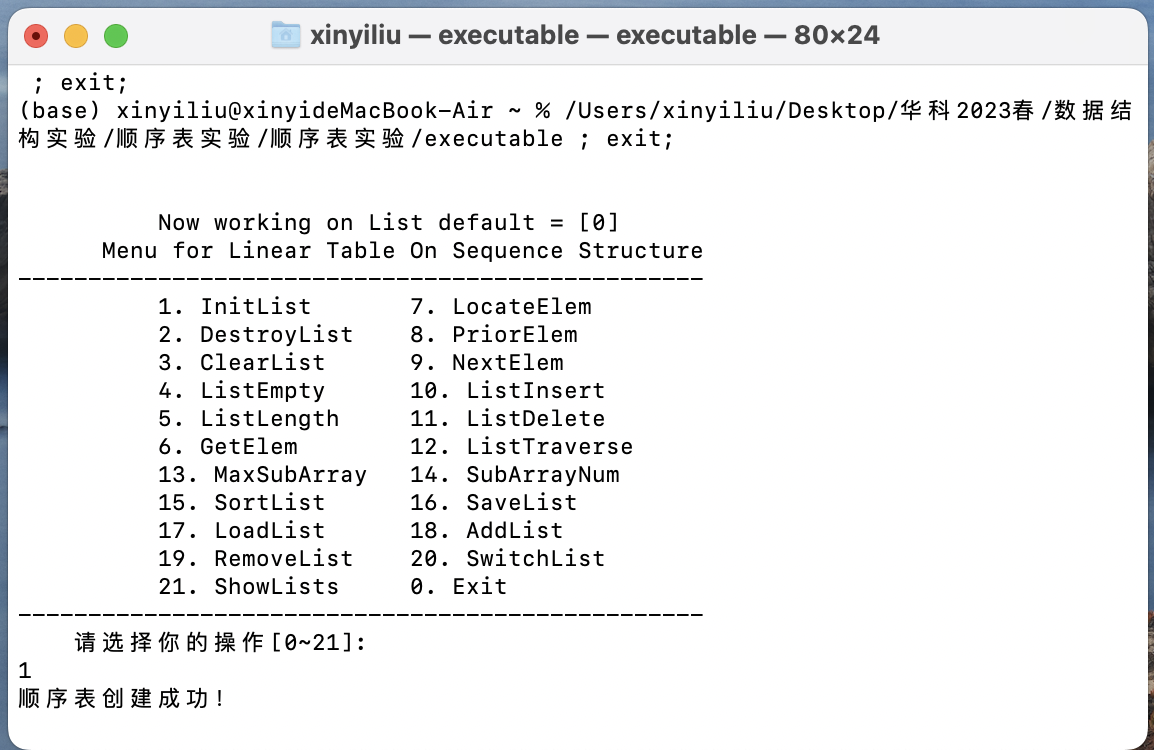
\includegraphics[width=0.8\linewidth]{images/截屏2023-06-01 18.21.29.png}
	\end{figure}
\FloatBarrier

\item \verb|ListInsert()|
	依次插入了元素1、2、3、4、5、6、7。
	\begin{figure}[!htb]
		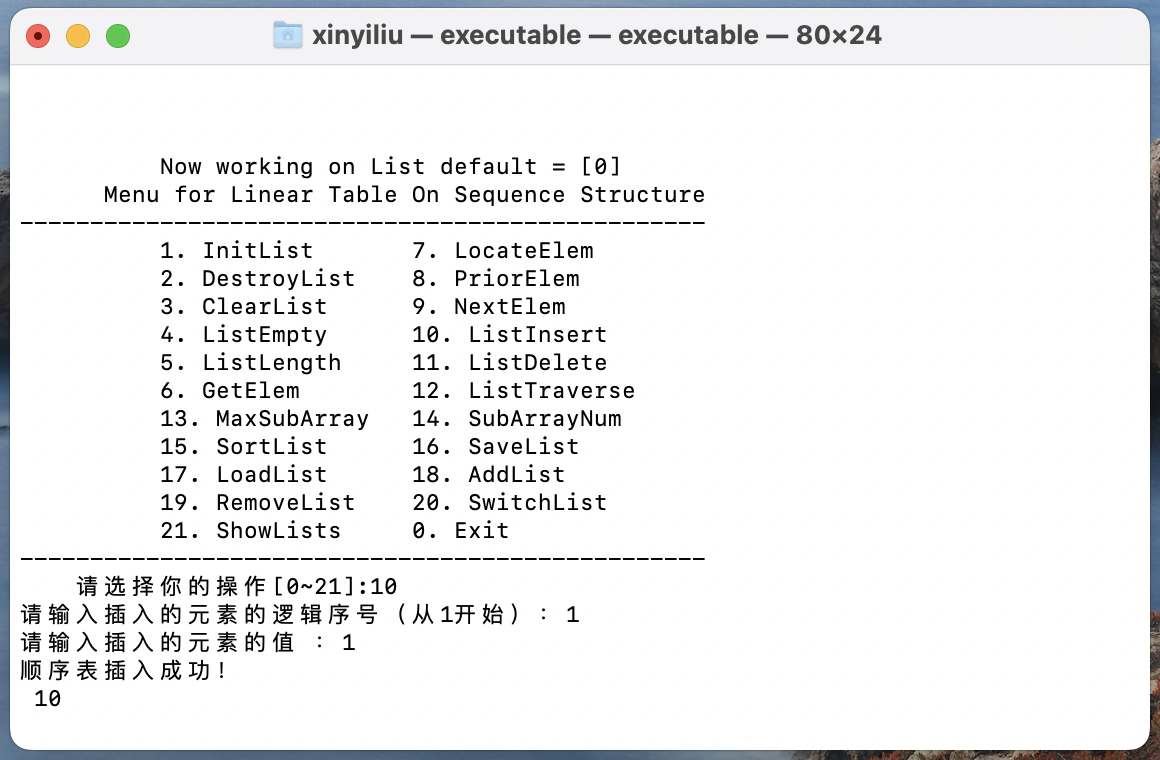
\includegraphics[width=0.8\linewidth]{images/截屏2023-06-01 18.21.51.png}
	\end{figure}
	\FloatBarrier
\newpage

\item \verb|ListEmpty()|
	\begin{figure}[!htb]
		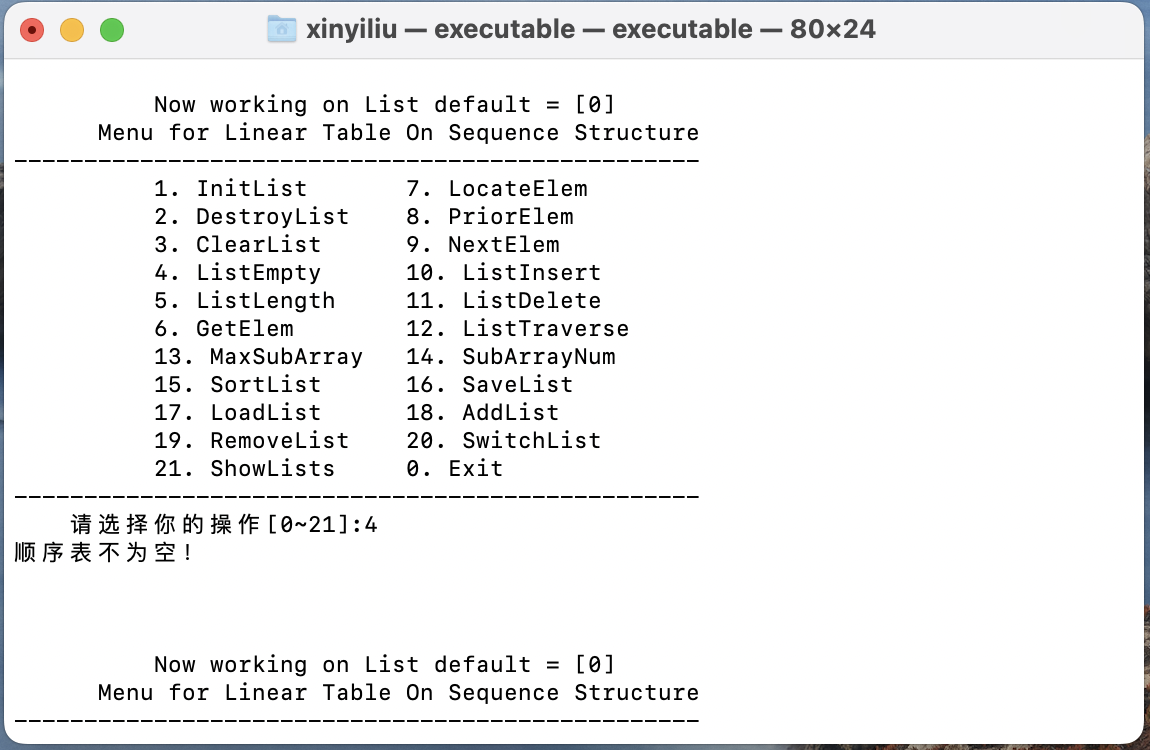
\includegraphics[width=0.8\linewidth]{images/截屏2023-06-01 18.23.33.png}
	\end{figure}
	\FloatBarrier

\item \verb|ListLength()|
	\begin{figure}[!htb]
		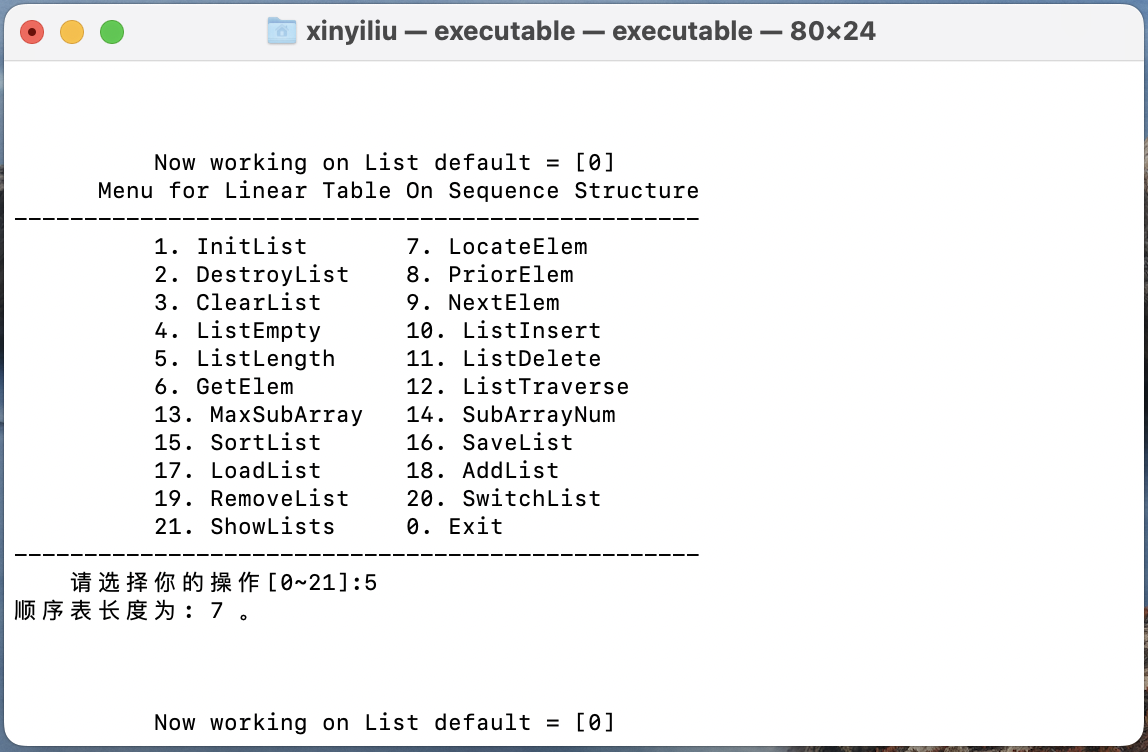
\includegraphics[width=0.8\linewidth]{images/截屏2023-06-01 18.23.42.png}
	\end{figure}
	\FloatBarrier

\newpage

\item \verb|GetElem()|
	\begin{figure}[!htb]
		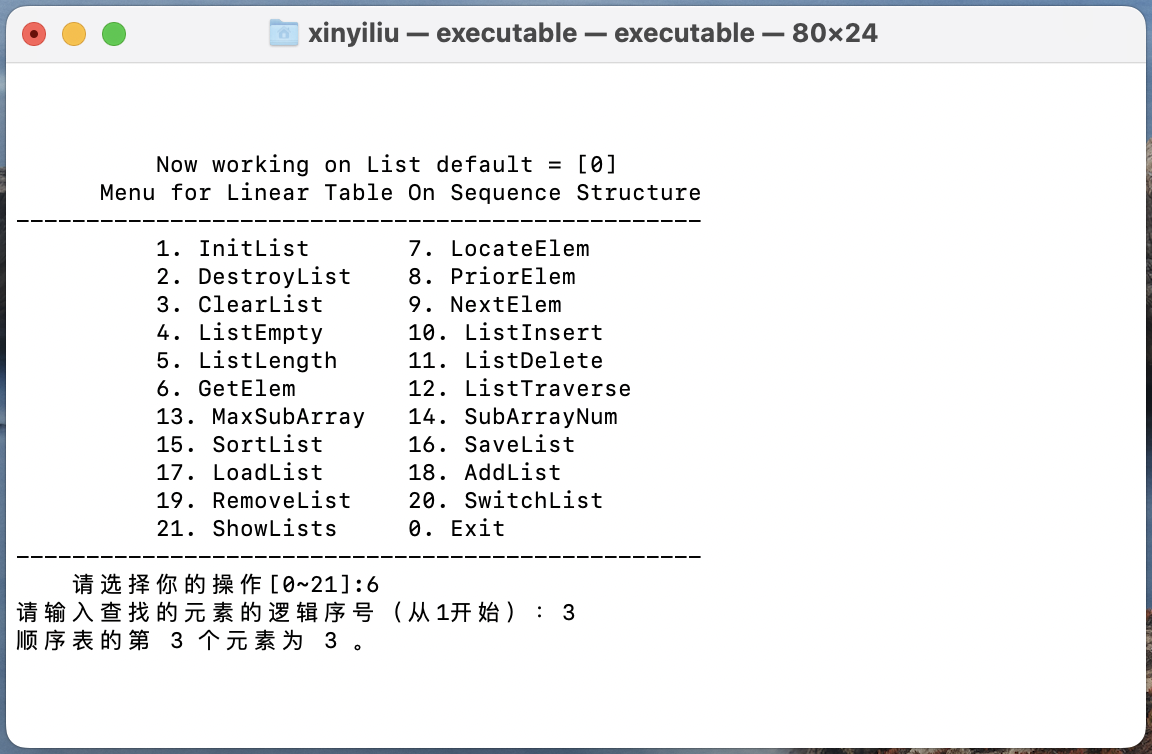
\includegraphics[width=0.8\linewidth]{images/截屏2023-06-01 18.24.07.png}
	\end{figure}
	\FloatBarrier

\item \verb|LocateElem()|
	\begin{figure}[!htb]
		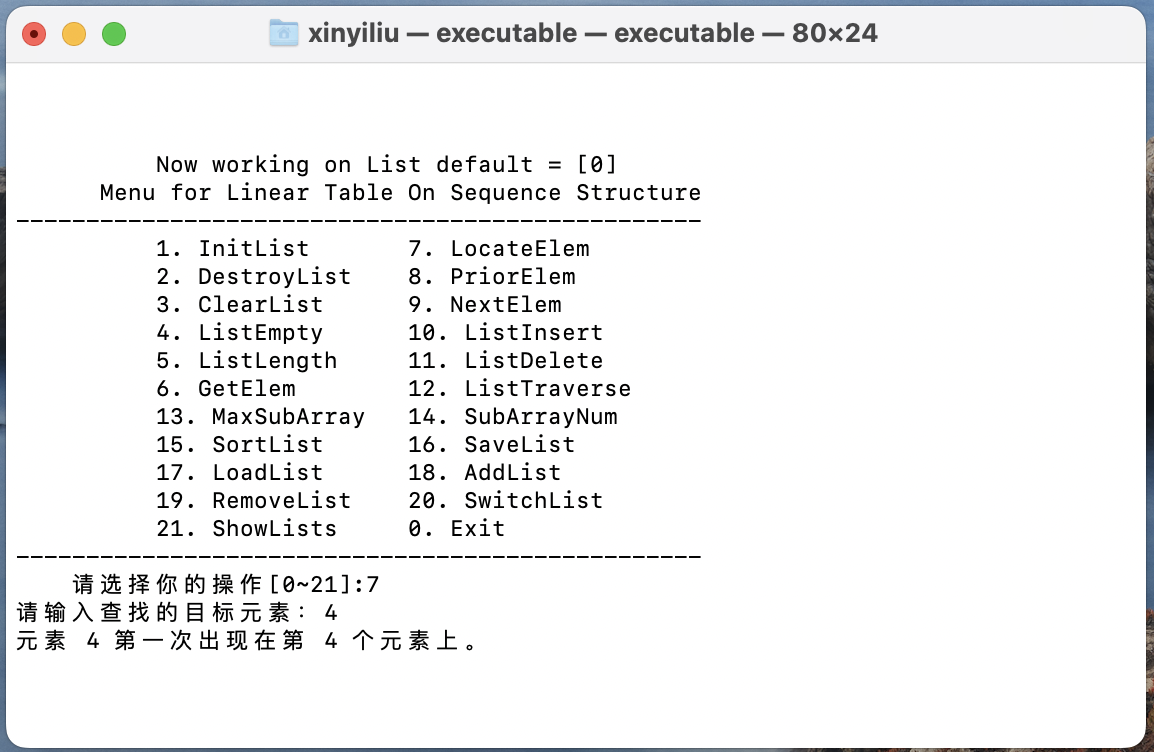
\includegraphics[width=0.8\linewidth]{images/截屏2023-06-01 18.22.44.png}
	\end{figure}
	\FloatBarrier
	
\newpage

\item \verb|PriorElem()|
	\begin{figure}[!htb]
		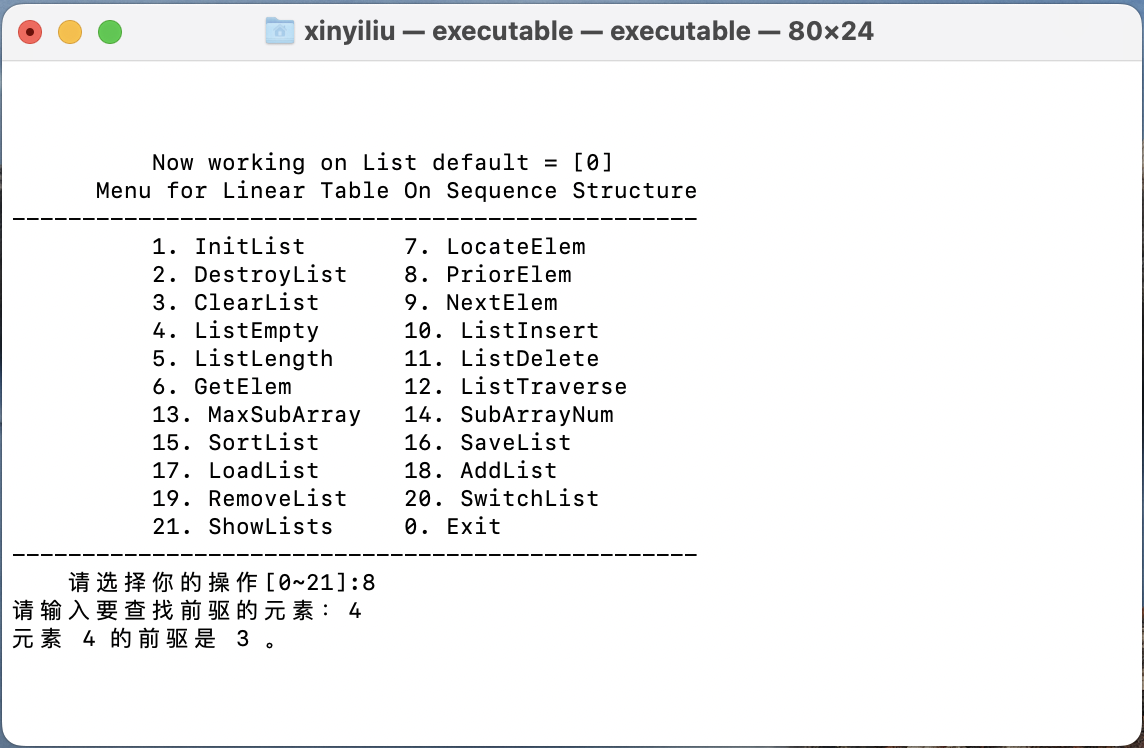
\includegraphics[width=0.8\linewidth]{images/截屏2023-06-01 18.22.56.png}
	\end{figure}
	\FloatBarrier

\item \verb|NextElem()|
	\begin{figure}[!htb]
		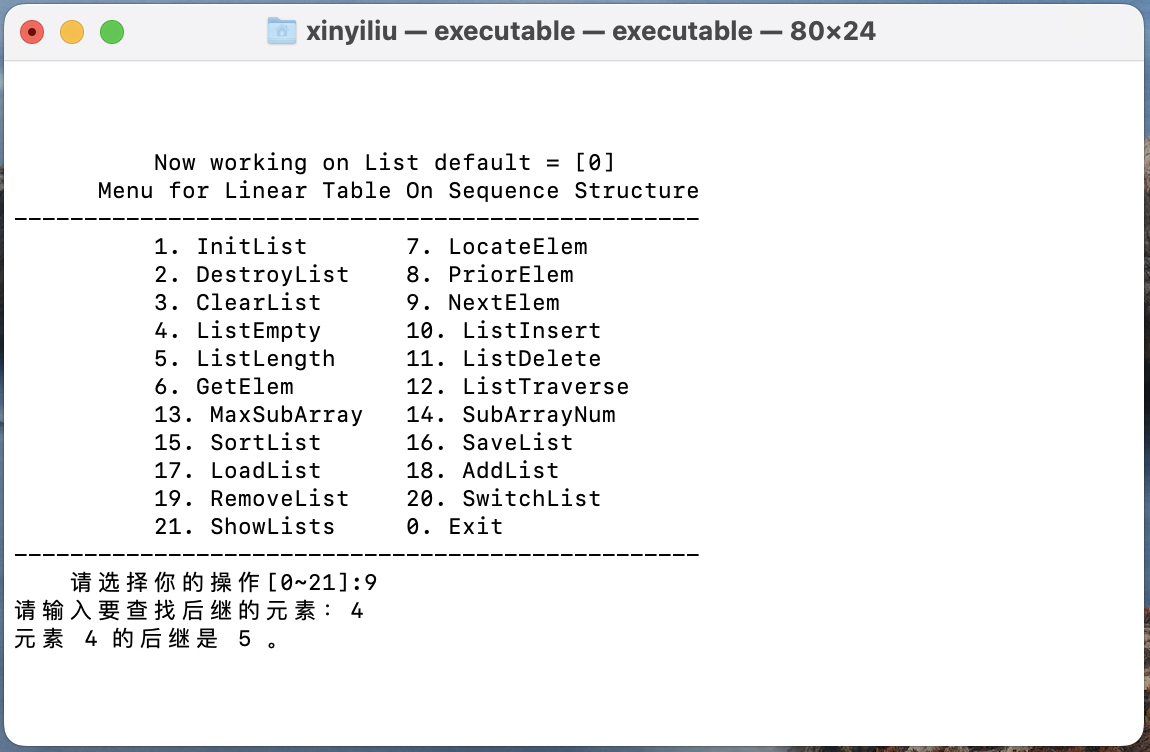
\includegraphics[width=0.8\linewidth]{images/截屏2023-06-01 18.23.17.png}
	\end{figure}
	\FloatBarrier
	
\newpage

\item \verb|ListDelete()|
	\begin{figure}[!htb]
		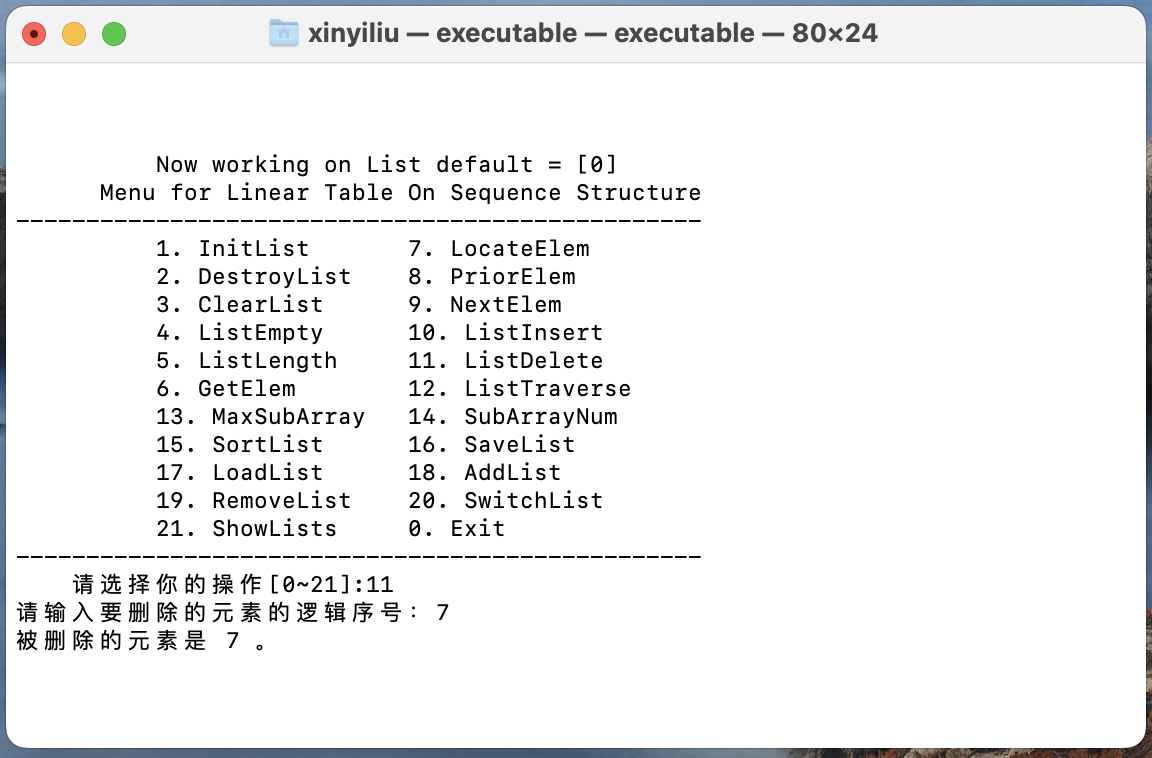
\includegraphics[width=0.8\linewidth]{images/截屏2023-06-01 18.23.53.png}
	\end{figure}
	\FloatBarrier

\item \verb|ListTraverse()|
	\begin{figure}[!htb]
		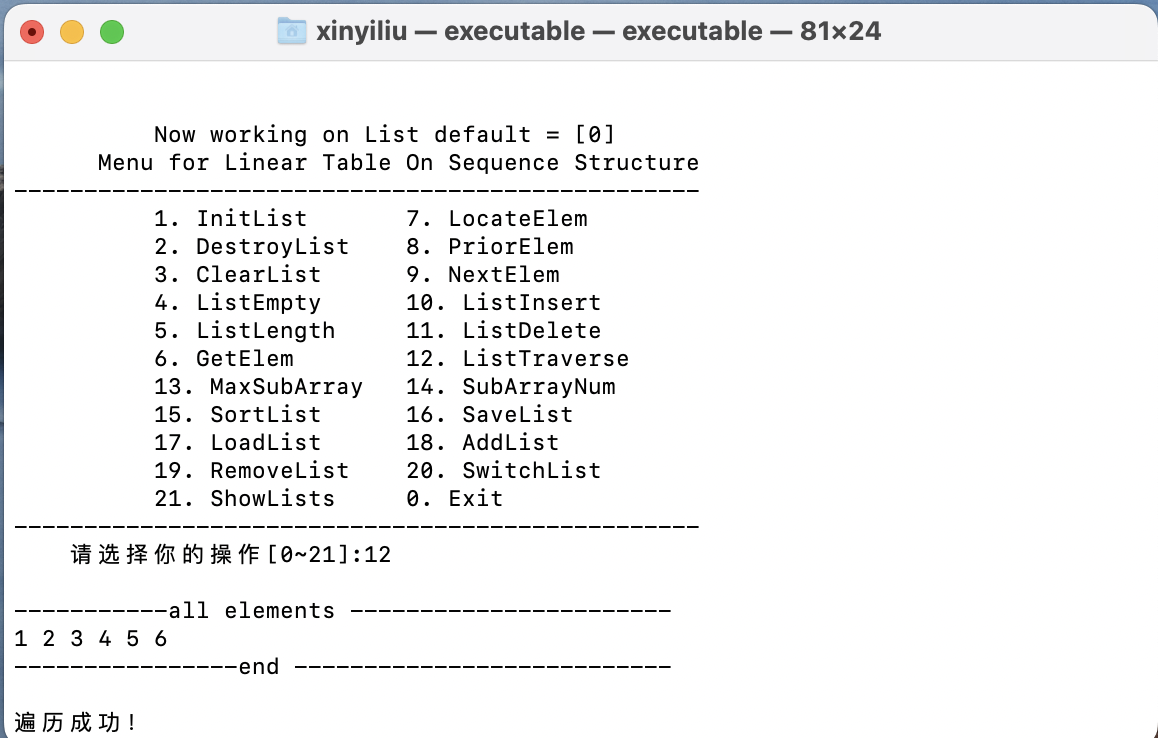
\includegraphics[width=0.8\linewidth]{images/截屏2023-06-01 21.46.52.png}
	\end{figure}
	\FloatBarrier

\newpage

\item \verb|ClearList()|
	\begin{figure}[!htb]
		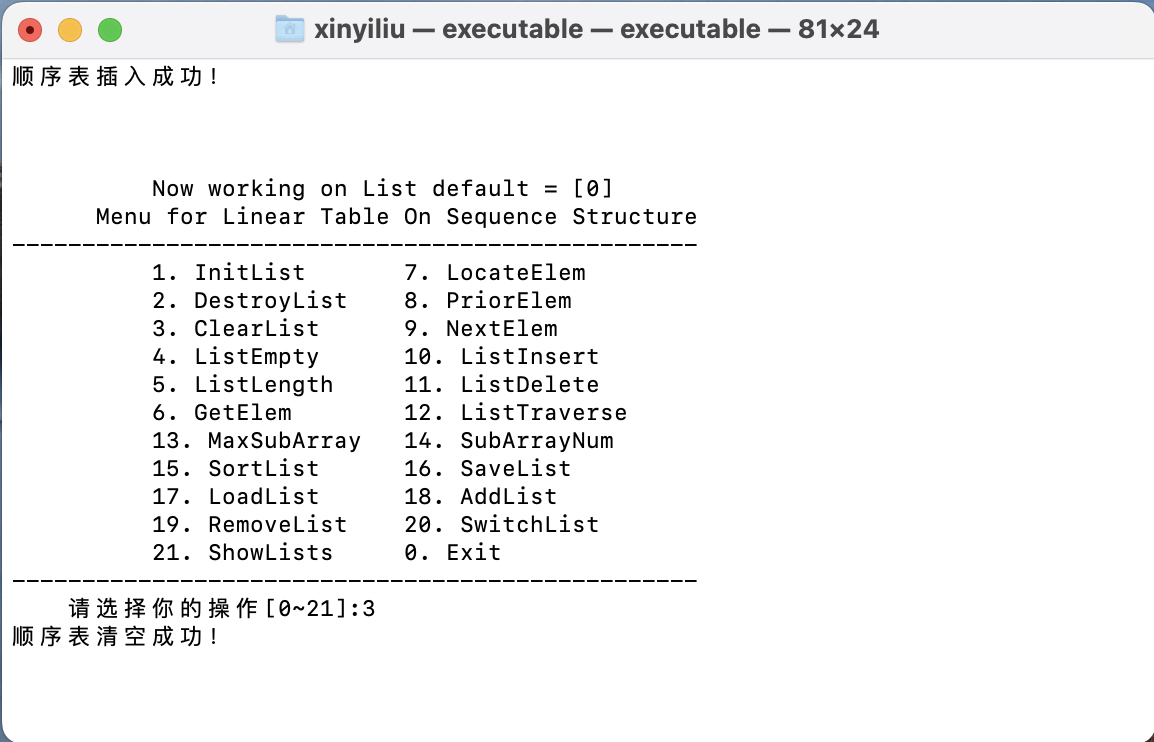
\includegraphics[width=0.8\linewidth]{images/截屏2023-06-01 21.56.17.png}
	\end{figure}
	\FloatBarrier

\item \verb|DestroyList()|
	\begin{figure}[!htb]
		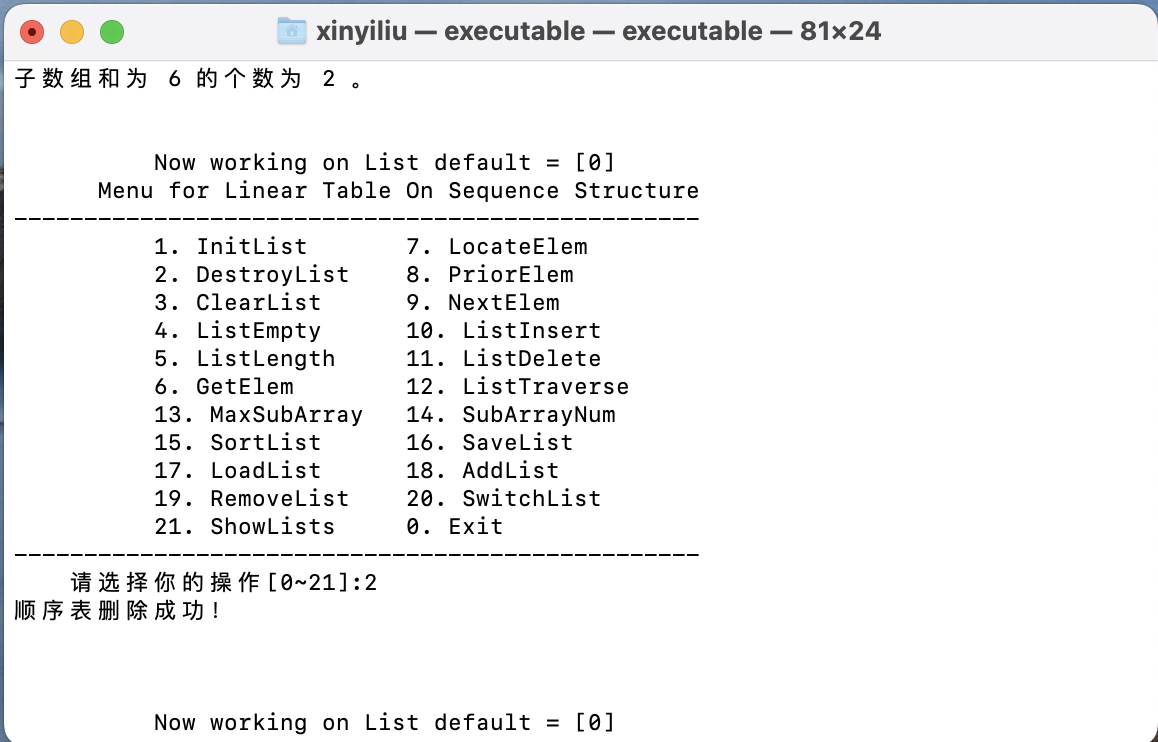
\includegraphics[width=0.8\linewidth]{images/截屏2023-06-01 18.24.43.png}
	\end{figure}
	\FloatBarrier

\end{enumerate}
\newpage

对顺序表{7,6,5,4,3,2,1}测试附加功能:
\begin{enumerate}

	\item \verb|MaxSubArray()|
	\begin{figure}[!htb]
		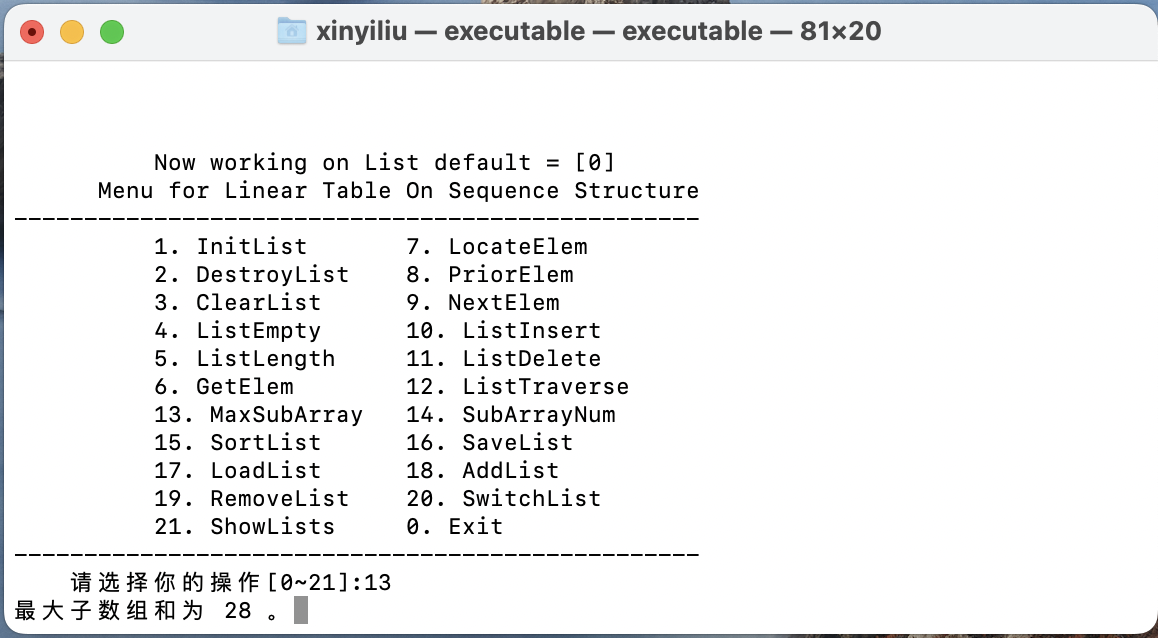
\includegraphics[width=0.8\linewidth]{images/截屏2023-06-01 22.14.26.png}
	\end{figure}
	\FloatBarrier

		
	\item \verb|SubArrayNum()|
	\begin{figure}[!htb]
		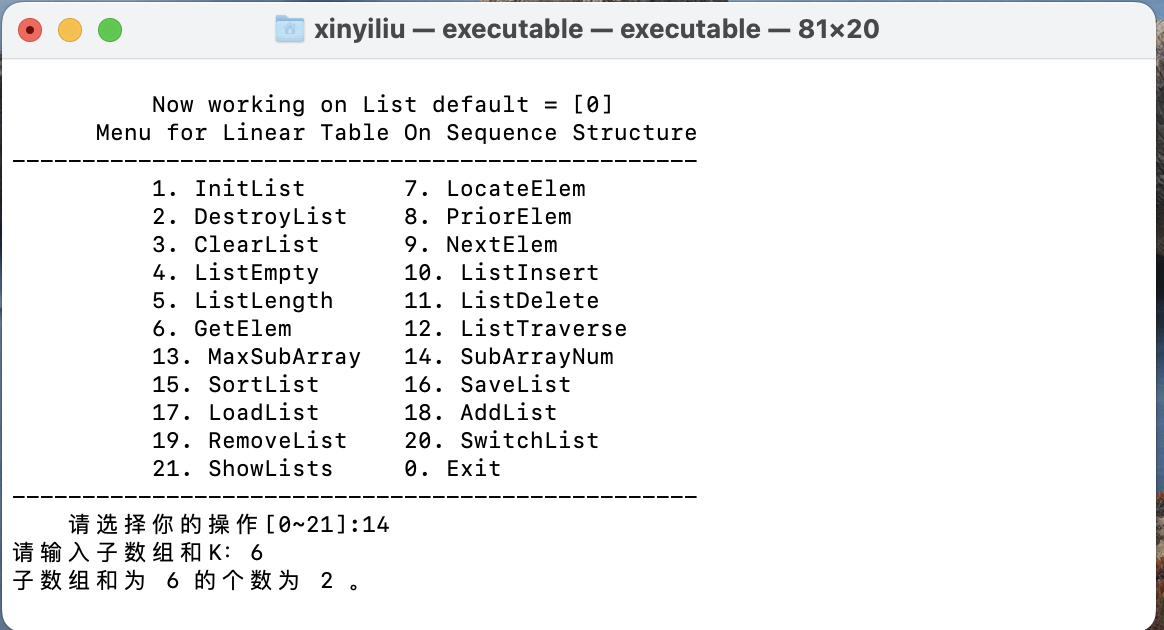
\includegraphics[width=0.8\linewidth]{images/截屏2023-06-01 22.14.44.png}
	\end{figure}
	\FloatBarrier

	\newpage

	\item \verb|SortList()|
	\begin{figure}[!htb]
		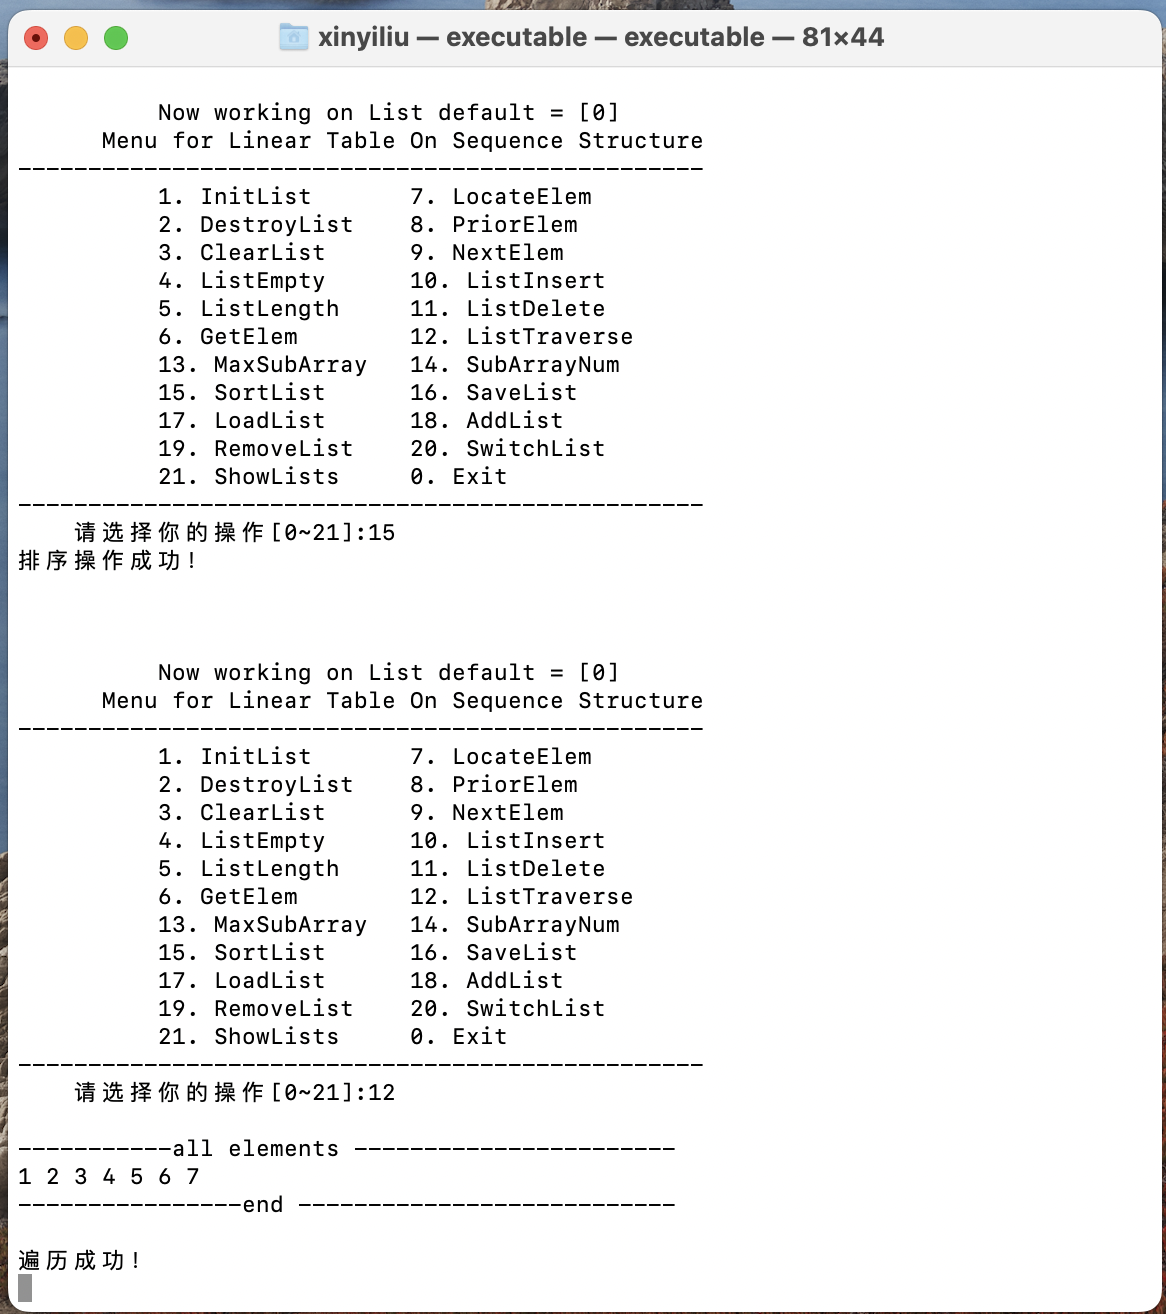
\includegraphics[width=0.8\linewidth]{images/截屏2023-06-01 22.16.47.png}
	\end{figure}
	\FloatBarrier
	
	\newpage

	\item \verb|SaveList()|、\verb|LoadList()|、\verb|List()|等多线性表管理功能。
	\begin{figure}[!htb]
		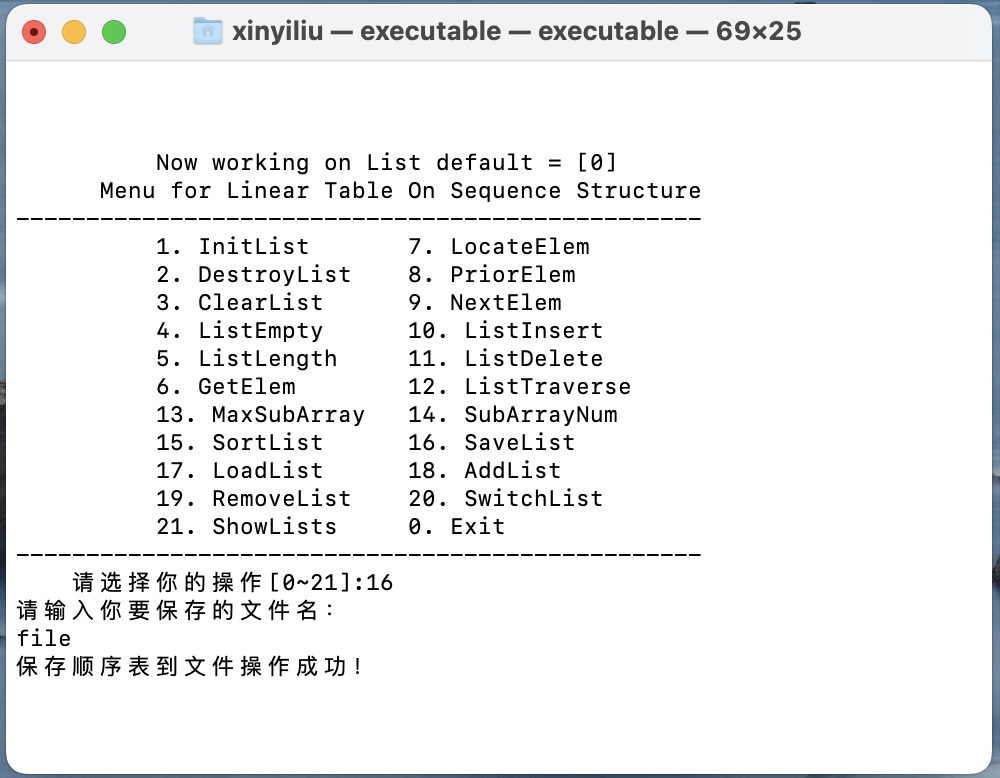
\includegraphics[width=0.8\linewidth]{images/截屏2023-06-01 22.19.25.png}
	\end{figure}
	\begin{figure}[!htb]
		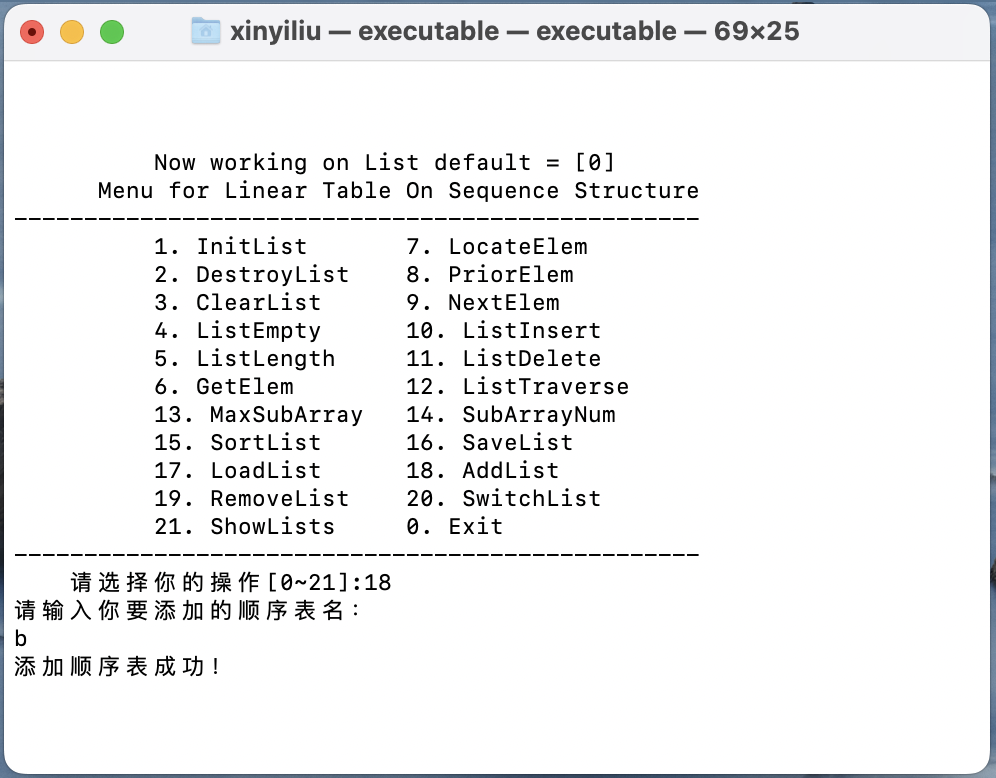
\includegraphics[width=0.8\linewidth]{images/截屏2023-06-01 22.19.36.png}
	\end{figure}
	\begin{figure}[!htb]
		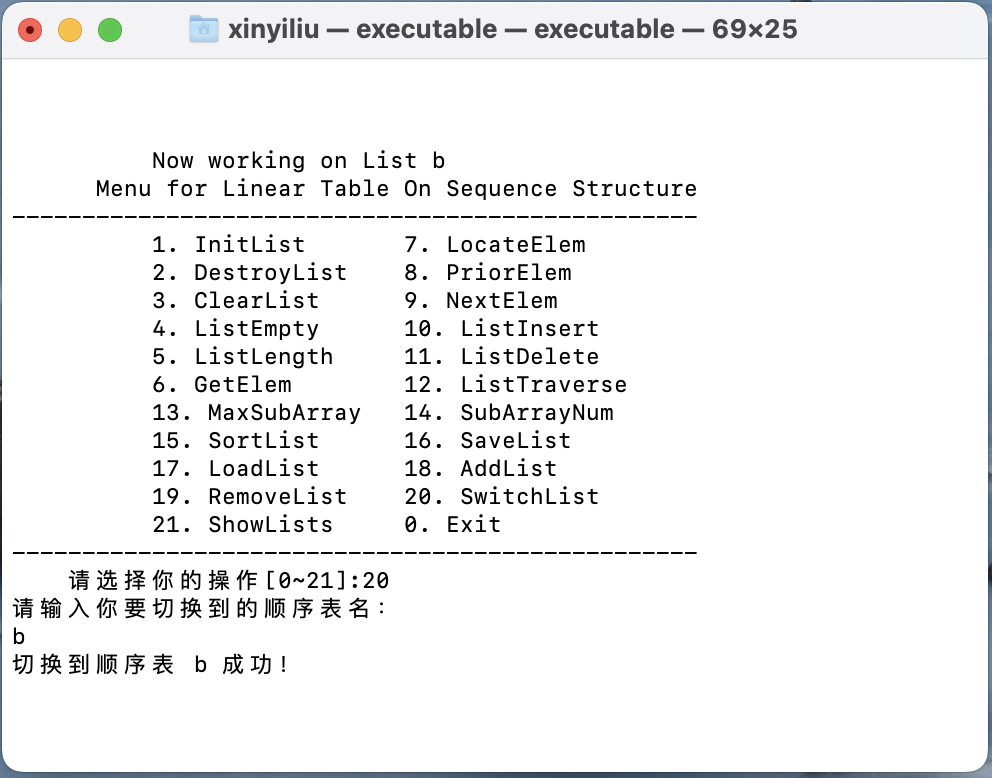
\includegraphics[width=0.8\linewidth]{images/截屏2023-06-01 22.19.46.png}
	\end{figure}
	\begin{figure}[!htb]
		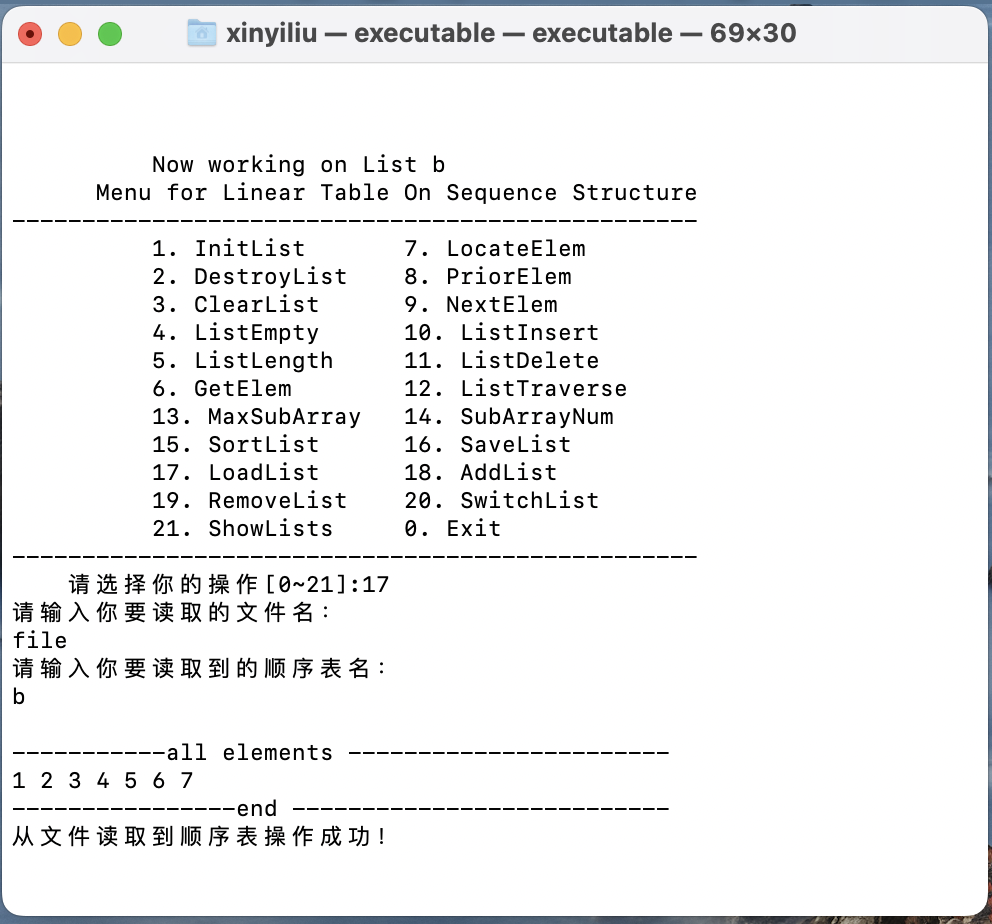
\includegraphics[width=0.8\linewidth]{images/截屏2023-06-01 22.20.01.png}
	\end{figure}
	\FloatBarrier
\end{enumerate}
\newpage
\section{基于二叉链表的二叉树实现}
要求构造一个具有菜单的功能演示系统。该演示系统实现二叉树管理。其中,在主函数中准备函数调用所需实参值、显示函数执行结果,并给出适当的操作提示。

实现依据最小完备性和常用性相结合的原则确定的创建二叉树、销毁二叉树、清空二叉树、判定空二叉树、求二叉树深度等12种基本运算,具体运算功能定义如下。

\subsection{问题描述}

要求构造一个具有菜单的功能演示系统。该演示系统实现二叉树管理。其中,在主函数中准备函数调用所需实参值、显示函数执行结果,并给出适当的操作提示。

实现依据最小完备性和常用性相结合的原则确定的创建二叉树、销毁二叉树、清空二叉树、判定空二叉树、求二叉树深度等12种基本运算,具体运算功能定义如下。

\begin{enumerate}
	\item 创建二叉树:函数名称是\verb|CreateBiTree(T,definition)|;初始条件是T不存在;\verb|definition| 给出二叉树\verb|T|的定义,如带空子树的二叉树前序遍历序列、或前序+中序、或后序+中序;操作结果是按\verb|definition|构造二叉树\verb|T|;(要求T中各结点关键字具有唯一性)
	\item 销毁二叉树:函数名称是\verb|DestroyBiTree(T)|;初始条件是二叉树\verb|T|已存在;操作结果是销毁二叉树\verb|T|;
	\item 清空二叉树:函数名称是\verb|ClearBiTree(T)|;初始条件是二叉树\verb|T|存在;操作结果是将二叉树\verb|T|清空;
	\item 判定空二叉树:函数名称是\verb|BiTreeEmpty(T)|;初始条件是二叉树\verb|T|存在;操作结果是若\verb|T|为空二叉树则返回\verb|TRUE|,否则返回\verb|FALSE|;
	\item 求二叉树深度:函数名称是\verb|BiTreeDepth(T)|;初始条件是二叉树\verb|T|存在;操作结果是返回\verb|T|的深度;
	\item 查找结点:函数名称是\verb|LocateNode(T,e)|;初始条件是二叉树\verb|T|已存在,\verb|e|是和\verb|T|中结点关键字类型相同的给定值;操作结果是返回查找到的结点指针,如无关键字为\verb|e|的结点,返回\verb|NULL|;
	\item 结点赋值:函数名称是\verb|Assign(T,e,value)|;初始条件是二叉树\verb|T|已存在,\verb|e|是和\verb|T|中结点关键字类型相同的给定值;操作结果是关键字为\verb|e|的结点赋值为\verb|value|;
	\item 获得兄弟结点:函数名称是\verb|GetSibling(T,e)|;初始条件是二叉树\verb|T|存在,\verb|e|是和\verb|T|中结点关键字类型相同的给定值;操作结果是返回关键字为\verb|e|的结点的(左或右)兄弟结点指针。若关键字为\verb|e|的结点无兄弟,则返回\verb|NULL|;
	\item 插入结点:函数名称是\verb|InsertNode(T,e,LR,c)|;初始条件是二叉树\verb|T|存在,\verb|e|是和\verb|T|中结点关键字类型相同的给定值,\verb|LR|为\verb|0|或\verb|1|,\verb|c|是待插入结点;操作结果是根据\verb|LR|为\verb|0|或者\verb|1|,插入结点\verb|c|到\verb|T|中,作为关键字为\verb|e|的结点的左或右孩子结点,结点\verb|e|的原有左子树或右子树则为结点\verb|c|的右子树(\verb|LR|为\verb|-1|时,作为根结点插入,原根结点作为\verb|c|的右子树);
	\item 删除结点:函数名称是\verb|DeleteNode(T,e)|;初始条件是二叉树\verb|T|存在,\verb|e|是和\verb|T|中结点关键字类型相同的给定值。操作结果是删除\verb|T|中关键字为\verb|e|的结点;同时,如果关键字为\verb|e|的结点度为\verb|0|,删除即可;如关键字为\verb|e|的结点度为\verb|1|,用关键字为\verb|e|的结点孩子代替被删除的\verb|e|位置;如关键字为\verb|e|的结点度为\verb|2|,用\verb|e|的左孩子代替被删除的\verb|e|位置,\verb|e|的右子树作为\verb|e|的左子树中最右结点的右子树;
	\item 前序遍历:函数名称是\verb|PreOrderTraverse(T,Visit)|;初始条件是二叉树\verb|T|存在,\verb|Visit|是一个函数指针的形参(可使用该函数对结点操作);操作结果:先序遍历,对每个结点调用函数\verb|Visit|一次且一次,一旦调用失败,则操作失败。
	\item 中序遍历:函数名称是\verb|InOrderTraverse(T,Visit)|;初始条件是二叉树\verb|T|存在,\verb|Visit|是一个函数指针的形参(可使用该函数对结点操作);操作结果是中序遍历\verb|T|,对每个结点调用函数\verb|Visit|一次且一次,一旦调用失败,则操作失败;
	\item 后序遍历:函数名称是\verb|PostOrderTraverse(T,Visit)|;初始条件是二叉树\verb|T|存在,\verb|Visit|是一个函数指针的形参(可使用该函数对结点操作);操作结果是后序遍历\verb|T|,对每个结点调用函数\verb|Visit|一次且一次,一旦调用失败,则操作失败。(注:前序、中序和后序三种遍历算法,要求至少一个用非递归算法实现)
	\item 按层遍历:函数名称是\verb|LevelOrderTraverse(T,Visit)|;初始条件是二叉树\verb|T|存在,\verb|Visit|是对结点操作的应用函数;操作结果是层序遍历\verb|T|,对每个结点调用函数\verb|Visit|一次且一次,一旦调用失败,则操作失败。
\end{enumerate}
此外,还在基础功能的基础上实现了附加功能:
\begin{enumerate}
	\item 最大路径和:函数名称是\verb|MaxPathSum(T)|,初始条件是二叉树\verb|T|存在;操作结果是返回根结点到叶子结点的最大路径和(以结点关键字为权重);
	\item 最近公共祖先:函数名称是\verb|LowestCommonAncestor(T,e1,e2)|;初始条件是二叉树\verb|T|存在;操作结果是该二叉树中\verb|e1|结点和\verb|e2|结点的最近公共祖先;
	\item 翻转二叉树:函数名称是\verb|InvertTree(T)|,初始条件是线性表\verb|L|已存在;操作结果是将\verb|T|翻转,使其所有结点的左右结点互换;
	\item 实现二叉树的文件形式保存,其中:
	\begin{itemize}
		\item 需要设计文件数据记录格式,以高效保存二叉树数据的完整信息;
		\item 需要设计二叉树文件保存和加载操作合理模式。
	\end{itemize}	
	\item 实现多个二叉树:创建、添加、移除二叉树。
\end{enumerate}
\subsection{系统设计}
\begin{enumerate}
	\item 函数名称:\verb|CreateBiTree(L,definition)|;

	初始条件:二叉树\verb|T|不存在;
	
	操作结果:按照定义前序遍历序列definition构造二叉树\verb|T|;
	
	设计思路:将\verb|CreateBiTree()| 作为一个递归函数 \\ \verb|RecurvalCreateBiTree(definition[], start)| \\的入口;由\verb|RecurvalCreateBiTree()|递归构造左右子树。

	\item 函数名称:\verb|DestroyBiTree(T)|;

	初始条件:二叉树\verb|T|存在;
	
	操作结果:销毁二叉树\verb|T|;
	
	设计思路:释放根结点内存后,调用\verb|DestroyBiTree()|销毁左右子树,当参数为空树时返回。
	
	\item 函数名称:\verb|ClearBiTree(T)|;
	
	初始条件:二叉树\verb|T|存在;

	操作结果:将二叉树的结点的所有数据域中的数据删除;

	设计思路:清空根结点后,递归清空左右子树,当参数为空树时返回。

	\item 函数名称:\verb|BiTreeEmpty|;
	
	初始条件:二叉树存在;

	操作结果:若\verb|T|为空二叉树则返回\verb|TRUE|,否则返回\verb|FALSE|;

	设计思路:如果\verb|T|是空指针则返回\verb|TRUE|,否则返回\verb|FALSE|;

	\item 函数名称:\verb|BiTreeDepth(T)|;
	
	初始条件:二叉树\verb|T|存在;

	操作结果:返回二叉树的深度;

	设计思路:递归求左右子树的深度,求它们的最大值\verb|D|,返回\verb|D+1|;

	\item 函数名称:\verb|LocateNode(T,e)|;
	
	初始条件:二叉树\verb|T|存在;

	操作结果:返回查找到的结点指针,如果无关键字为\verb|e|的结点返回NULL;

	设计思路:先查找根结点,再递归查找左右子树,返回查找到的指针值,如果参数是空树返回NULL;

	\item 函数名称:\verb|Assign(T,e,value)|;
	
	初始条件:二叉树\verb|T|存在;

	操作结果:关键字为e的结点赋值为value;

	设计思路:调用函数\verb|LocateNode(T,e)|查找到关键字为\verb|e|的结点,再赋值为\verb|value|;

	\item 函数名称:\verb|GetSibling(T,e)|;
	
	初始条件:二叉树\verb|T|存在;

	操作结果:返回关键字为\verb|e|的结点的兄弟结点指针,如果关键字为\verb|e|的结点无兄弟,则返回\verb|NULL|;

	设计思路:编写函数\verb|LocateParents(T,e)|,该函数返回关键字为\verb|e|的双亲结点指针,再由双亲结点找到关键字为\verb|e|结点的兄弟结点,并返回指向兄弟结点的指针值;

	\item 函数名称:\verb|InsertNode(T,e,LR,c)|;
	
	初始条件:二叉树\verb|T|存在;

	操作结果:根据\verb|LR|为\verb|0|或者\verb|1|,插入结点\verb|c|到\verb|T|中,作为关键字为\verb|e|的结点的左或右孩子结点,结点\verb|e|的原有左子树或右子树则为结点\verb|c|的右子树,
	\verb|LR|为\verb|-1|时,作为根结点插入,原根结点作为\verb|c|的右子树。

	设计思路:先调用\verb|LocateNode|找到关键字为\verb|e|的结点,再按要求插入结点。

	\item 函数名称:\verb|DeleteNode(T,e)|;
	
	初始条件:二叉树\verb|T|存在;

	操作结果:操作结果是删除\verb|T|中关键字为\verb|e|的结点;同时,如果关键字为\verb|e|的结点度为\verb|0|,即删除,如关键字为\verb|e|的结点度为\verb|1|,用关键字为\verb|e|的结点的孩子代替被删除的\verb|e|位置;如关键字为\verb|e|的结点度为\verb|2|,用\verb|e|的左孩子代替被删除的\verb|e|位置,\verb|e|的右子树作为\verb|e|的左子树中最右结点的右子树;

	设计思路:先调用\verb|LocateNode|找到关键字为\verb|e|的结点,再按要求删除结点。

	\item 函数名称:\verb|PreOrderTraverse(T)|;
	
	初始条件:二叉树\verb|T|存在;

	操作结果:按前序遍历序列依次调用\verb|visit()|函数访问树上的结点;

	设计思路:先访问根结点,再前序遍历左子树,再前序遍历右子树;

	\item 函数名称:\verb|InOrderTraverse(T)|;
	
	初始条件:二叉树\verb|T|存在;

	操作结果:按中序遍历序列依次调用\verb|visit()|函数访问树上的结点;

	设计思路:先中序遍历左子树,再访问根结点,再中序遍历右子树(非递归实现,用一个栈确定访问的顺序);

	\item 函数名称:\verb|PostOrderTraverse(T)|;
	
	初始条件:二叉树\verb|T|存在;

	操作结果:按后序遍历序列依次调用\verb|visit()|函数访问树上的结点;

	设计思路:先后序遍历左子树,再后序遍历右子树,再访问根结点;

	\item 函数名称:\verb|LevelOrderTraverse(L)|;

	初始条件:二叉树\verb|T|存在;

	操作结果:按层次顺序调用\verb|visit()|函数访问树上的结点;

	设计思路:用一个队列保存被访问结点的子结点来实现按层遍历;

	\item 函数名称:\verb|MaxPathSum(T)|;
	
	初始条件:二叉树\verb|T|存在;

	操作结果:返回最大路径和;

	设计思路:对左、右子树递归调用\verb|MaxPathSum()|,求其最大值\verb|D|,返回\verb|D+1|;

	\item 函数名称:\verb|LowestCommonAncestor(T,e1,e2)|;
	
	初始条件:二叉树\verb|T|存在;

	操作结果:返回最近的公共祖先;
	
	设计思路:迭代调用\verb|LocateParents|上溯,找到\verb|e1|、\verb|e2|到根结点的路径交汇处;

	\item 函数名称:\verb|InvertTree|;
	
	初始条件:二叉树\verb|T|存在;

	操作结果:将二叉树的所有结点左右子树交换;
	
	设计思路:先交换根结点左右孩子,再递归翻转左子树、右子树;
\end{enumerate}
\newpage
\subsection{系统实现}
见《附录C 基于二叉链表二叉树实现的源程序》。
\subsection{系统测试}
先插入结点再依次测试各项功能;下面给出了基础功能的测试截图,测试是按图片的顺序进行的。
\begin{enumerate}
	\item \verb|CreateBiTree()|
		\begin{figure}[!htb]
			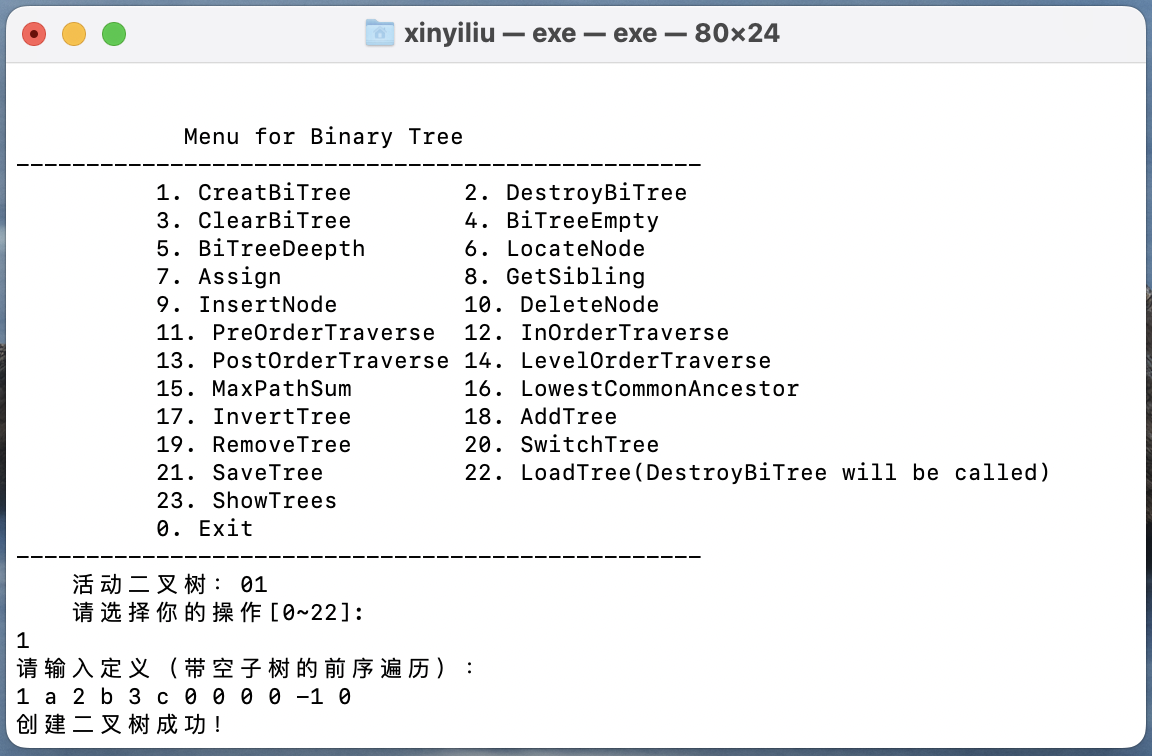
\includegraphics[width=0.8\linewidth]{images/img02/截屏2023-06-04 21.13.12.png}
		\end{figure}
	\FloatBarrier
	
	\item \verb|BiTreeEmpty()|
		\begin{figure}[!htb]
			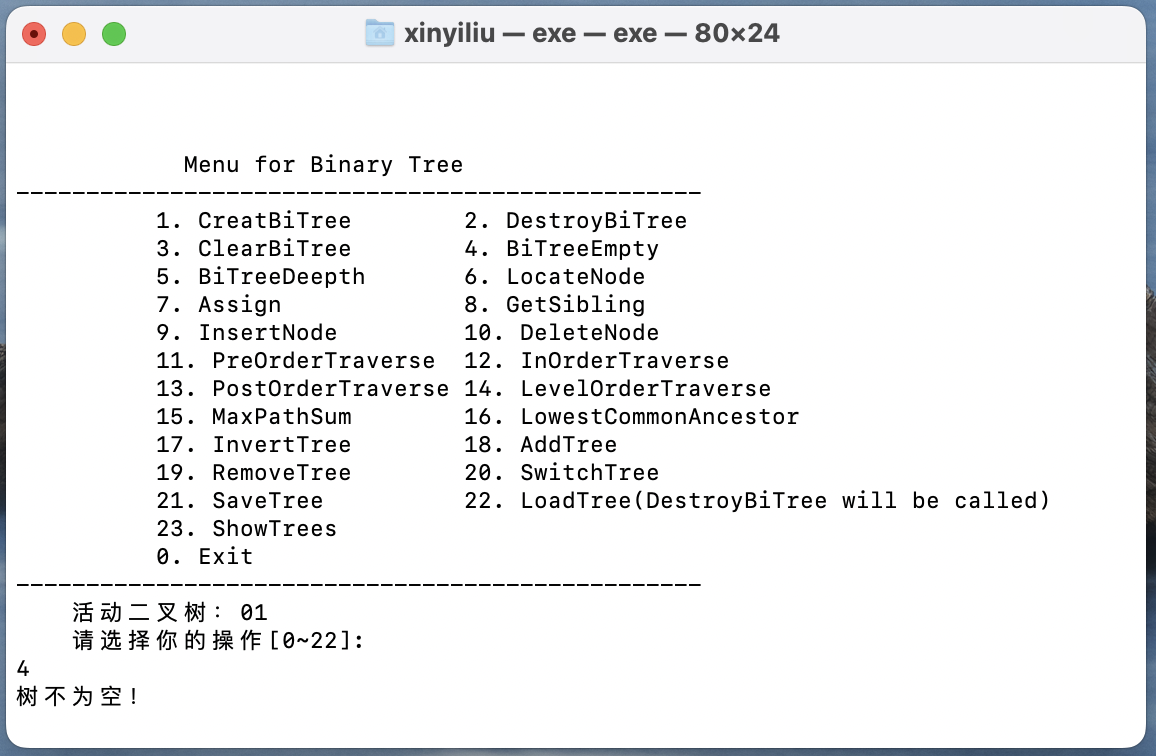
\includegraphics[width=0.8\linewidth]{images/img02/截屏2023-06-04 21.13.22.png}
		\end{figure}
		\FloatBarrier
	\newpage
	\item \verb|LocateNode()|
		\begin{figure}[!htb]
			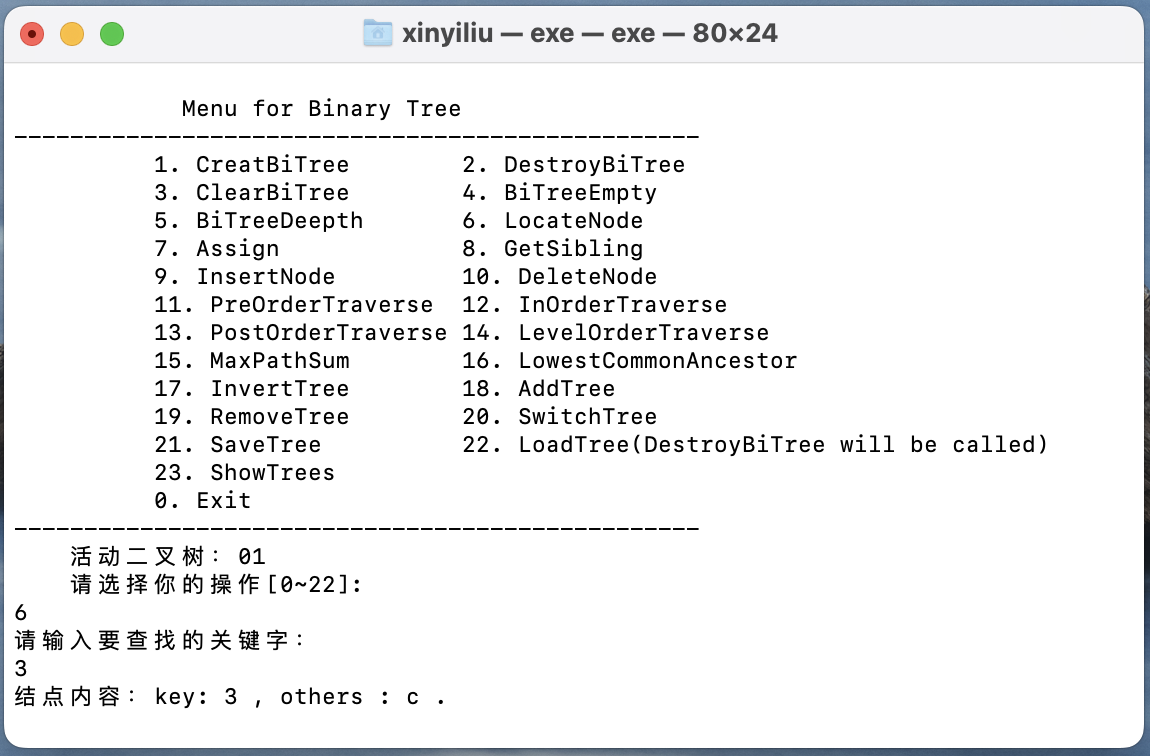
\includegraphics[width=0.8\linewidth]{images/img02/截屏2023-06-04 21.13.38.png}
		\end{figure}
	\FloatBarrier
	
	\item \verb|Assign()|
		\begin{figure}[!htb]
			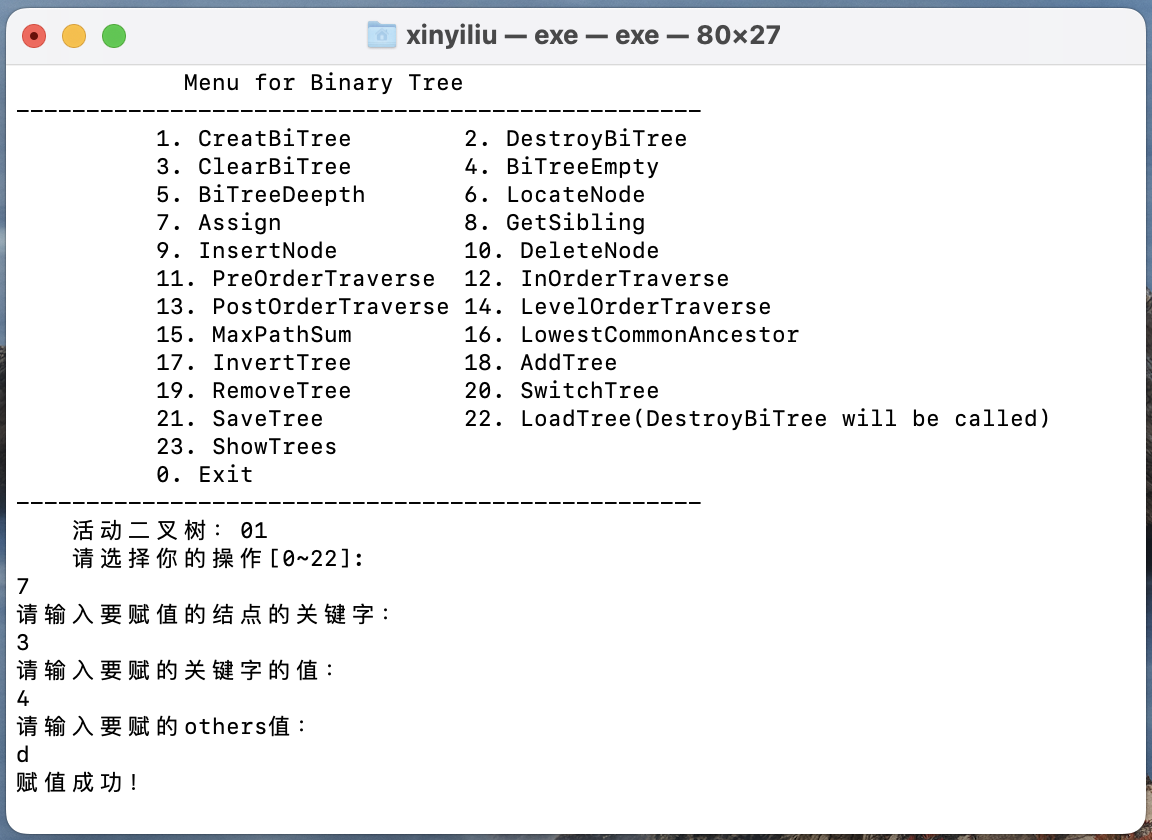
\includegraphics[width=0.8\linewidth]{images/img02/截屏2023-06-04 21.13.56.png}
		\end{figure}
		\FloatBarrier
	\newpage
	\item \verb|GetSibling()|
		\begin{figure}[!htb]
			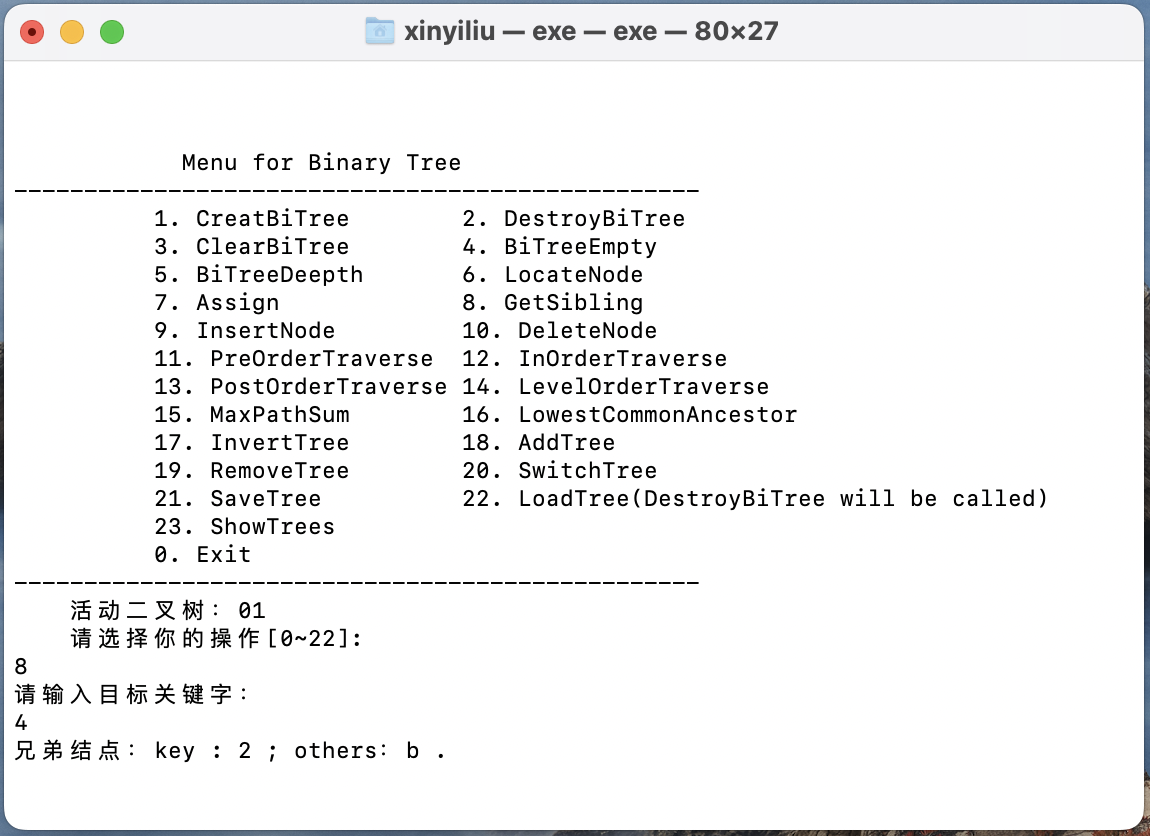
\includegraphics[width=0.8\linewidth]{images/img02/截屏2023-06-04 21.14.08.png}
		\end{figure}
	\FloatBarrier
	
	\item \verb|InsertNode()|
		\begin{figure}[!htb]
			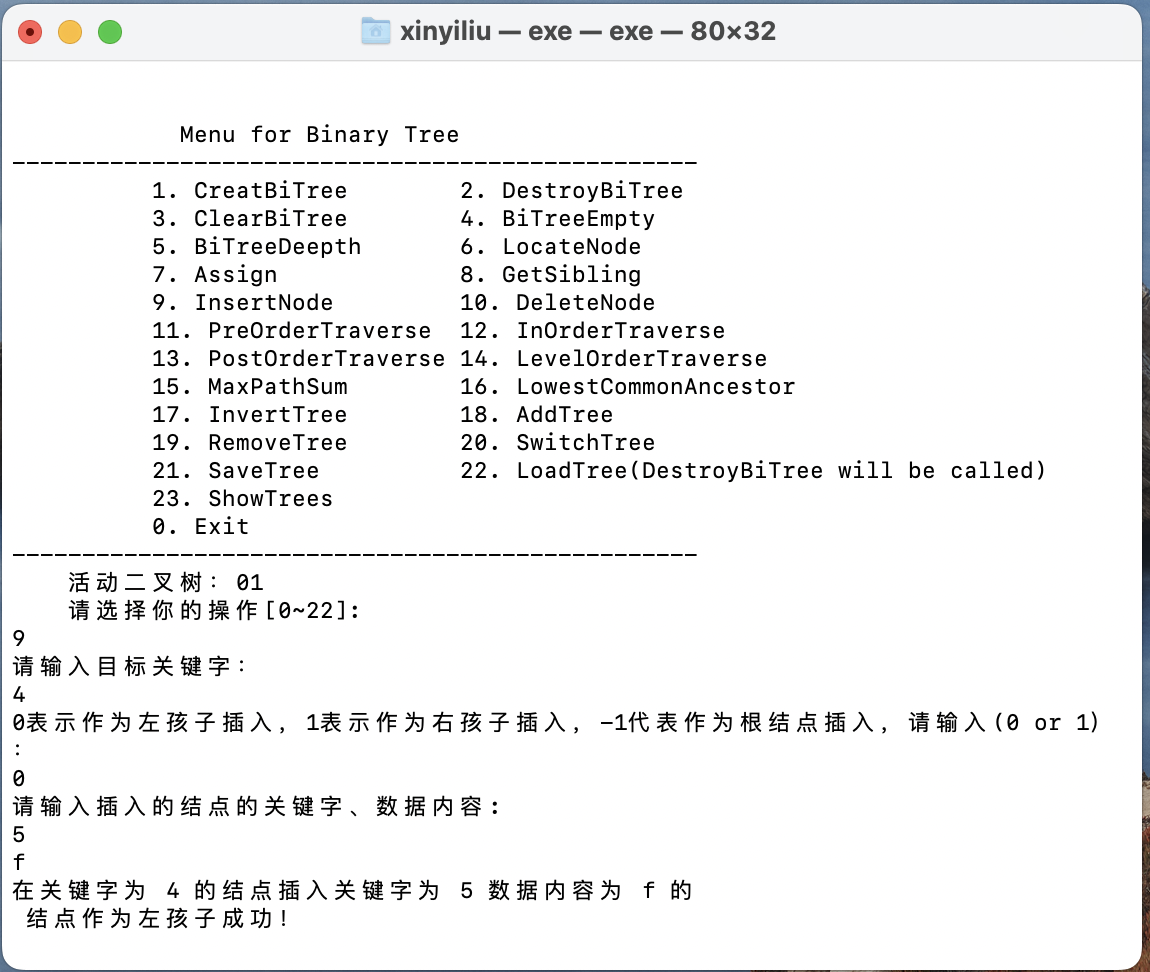
\includegraphics[width=0.8\linewidth]{images/img02/截屏2023-06-04 21.14.24.png}
		\end{figure}
		\FloatBarrier
	\newpage
	\item \verb|DeleteNode()|
		\begin{figure}[!htb]
			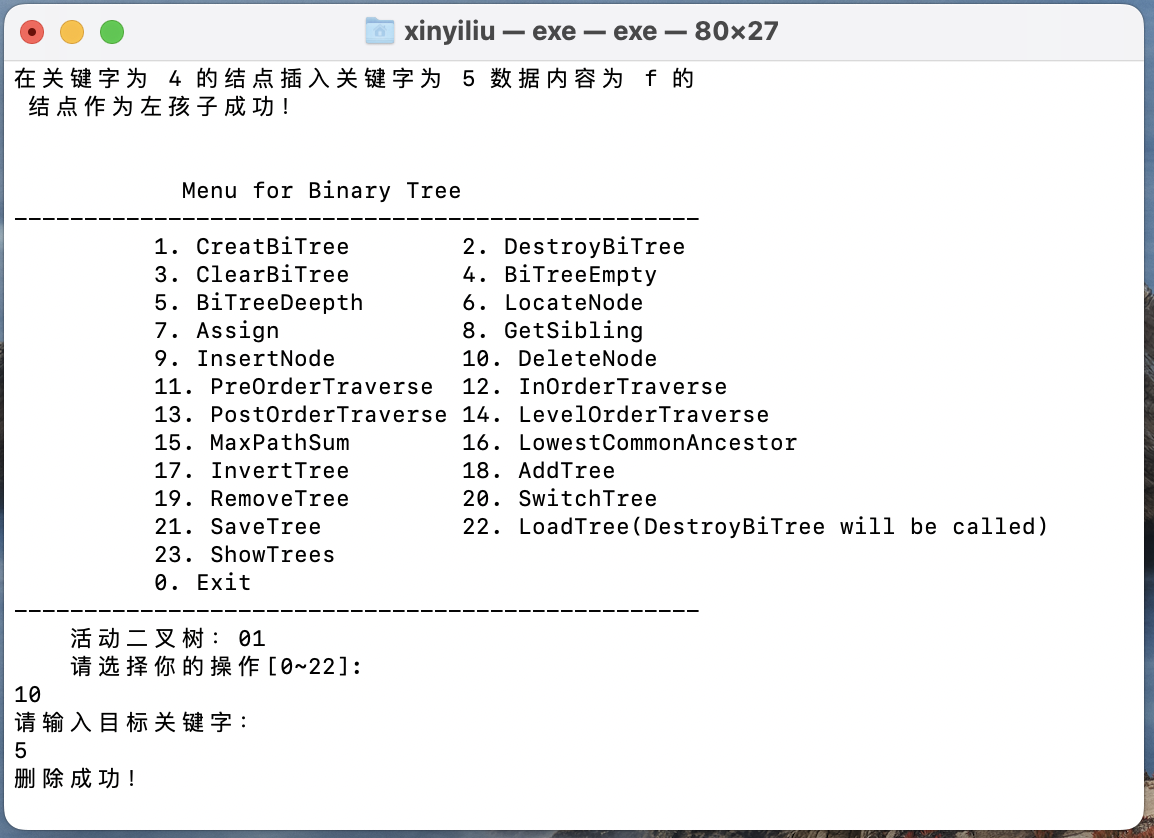
\includegraphics[width=0.8\linewidth]{images/img02/截屏2023-06-04 21.14.48.png}
		\end{figure}
	\FloatBarrier
	
	\item \verb|PreOrderTraverse()|
		\begin{figure}[!htb]
			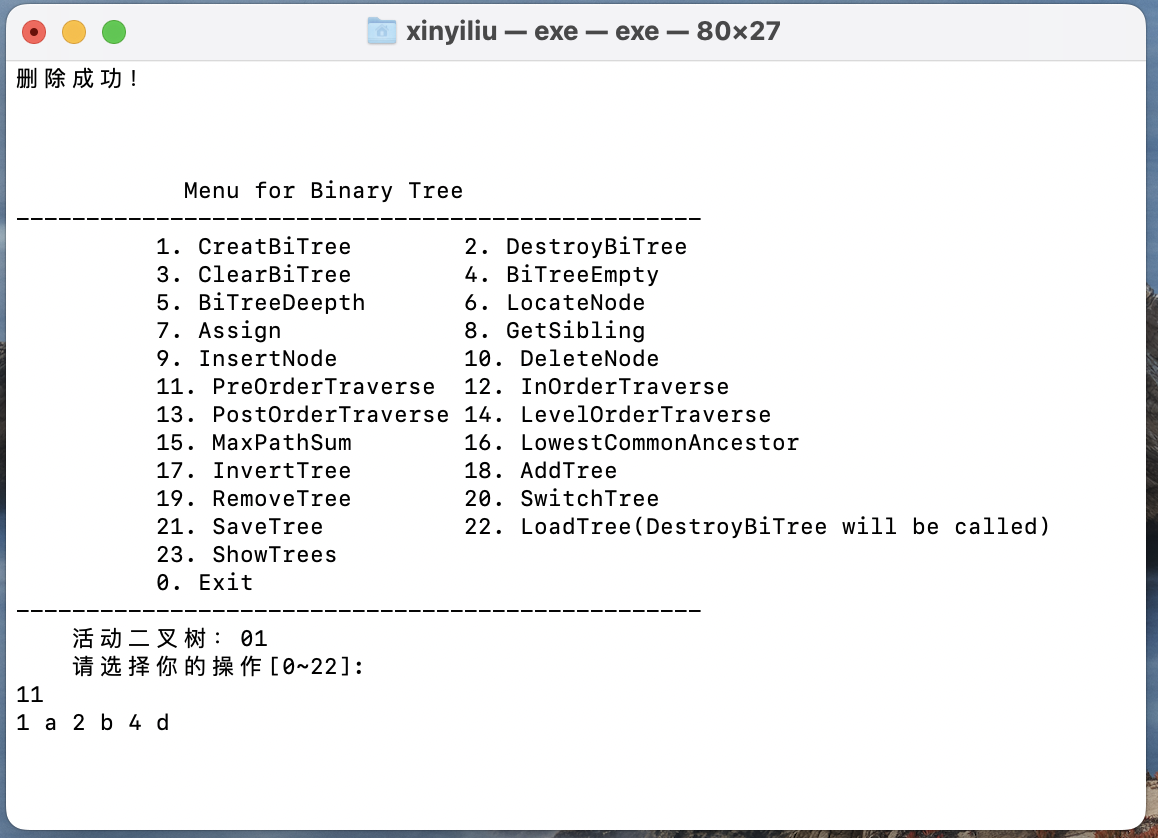
\includegraphics[width=0.8\linewidth]{images/img02/截屏2023-06-04 21.15.01.png}
		\end{figure}
		\FloatBarrier
	\newpage
	\item \verb|InOrderTraverse()|
		\begin{figure}[!htb]
			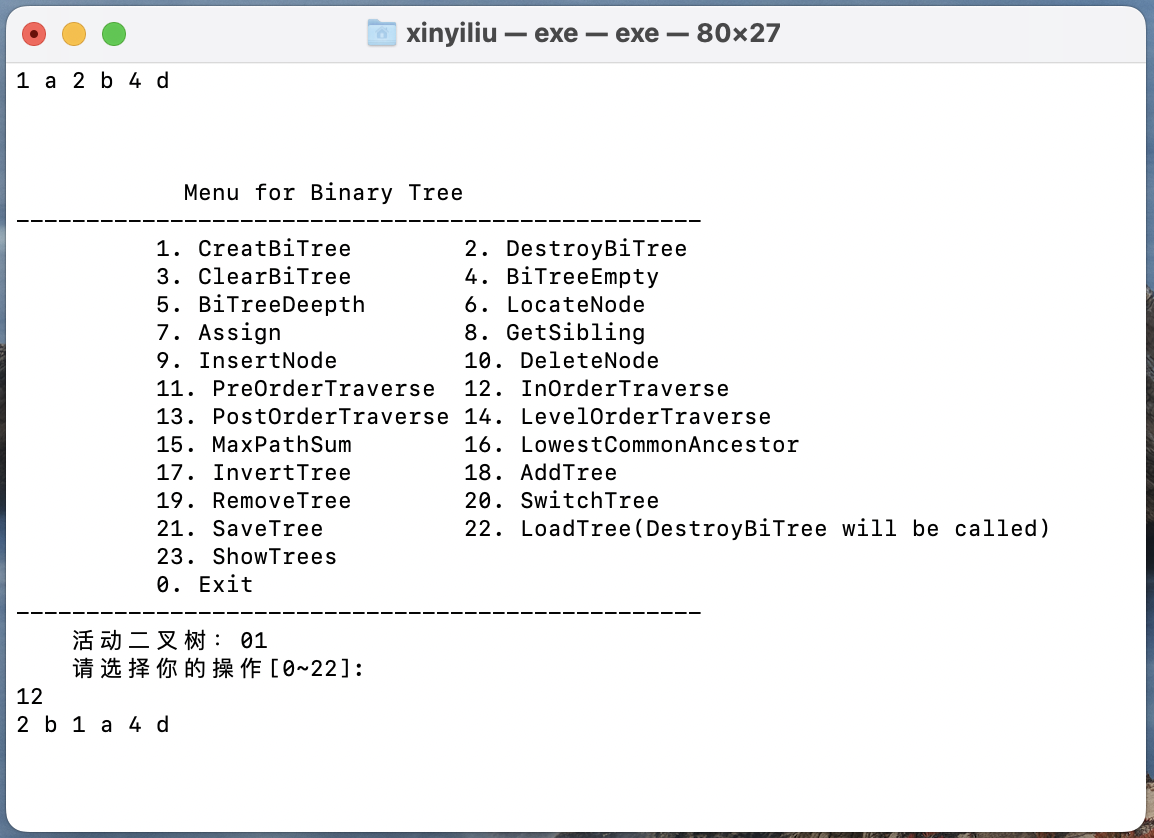
\includegraphics[width=0.8\linewidth]{images/img02/截屏2023-06-04 21.15.08.png}
		\end{figure}
	\FloatBarrier
	
	\item \verb|PostOrderTraverse()|
		\begin{figure}[!htb]
			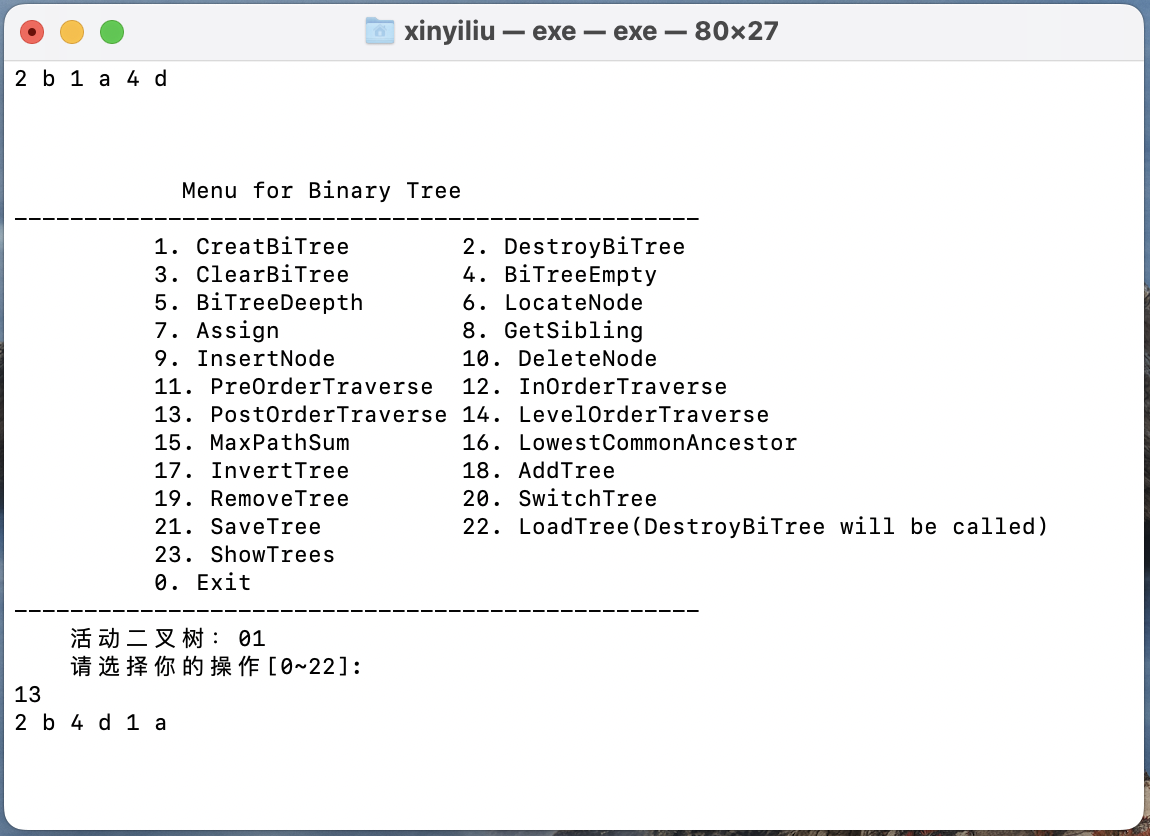
\includegraphics[width=0.8\linewidth]{images/img02/截屏2023-06-04 21.15.22.png}
		\end{figure}
		\FloatBarrier
	\newpage
	\item \verb|LevelOrderTraverse()|
		\begin{figure}[!htb]
			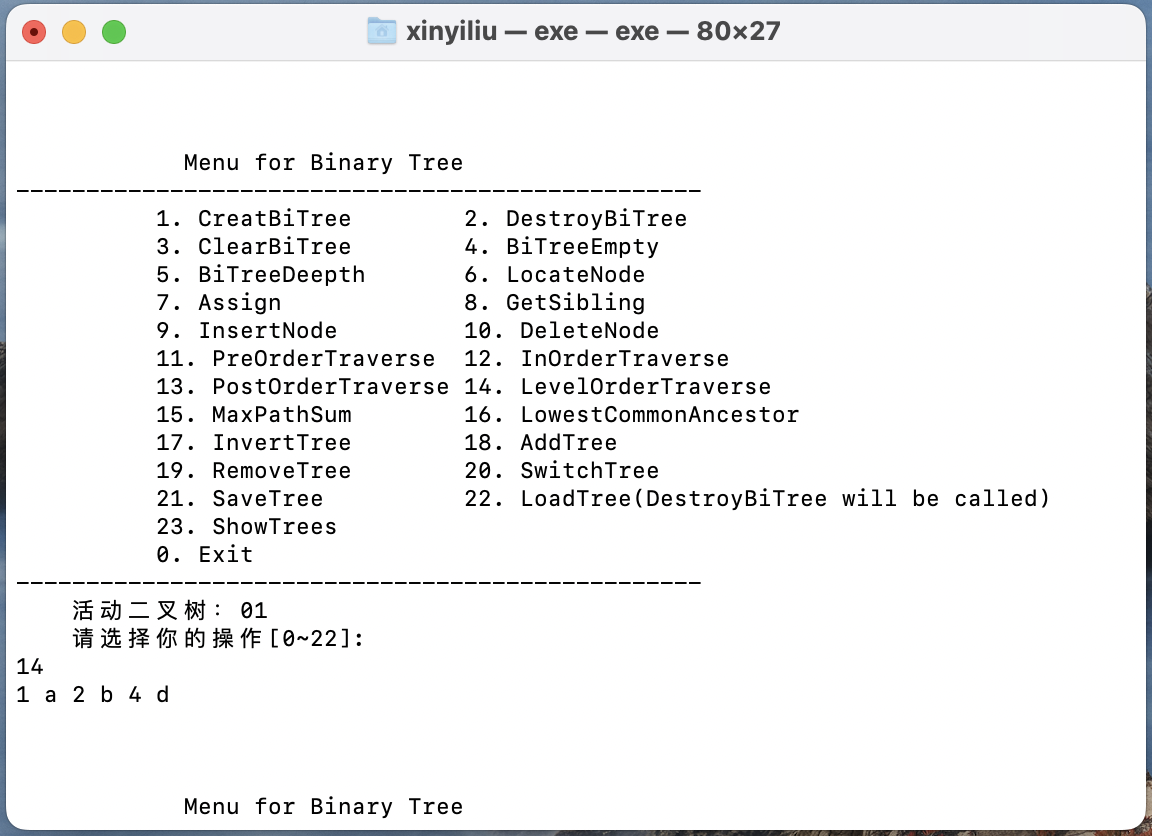
\includegraphics[width=0.8\linewidth]{images/img02/截屏2023-06-04 21.15.30.png}
		\end{figure}
	\FloatBarrier
	\newpage
\end{enumerate}
\newpage
\section{实验总结}

\section{附录A 基于顺序存储结构线性表实现的源程序}
\begin{lstlisting}
	#include <stdio.h>
	#include <stdlib.h>
	#include <string.h>
	#include <limits.h>
	#define TRUE 1
	#define FALSE 0
	#define OK 1
	#define ERROR 0
	#define INFEASIBLE -1
	#define OVERFLOW -2
	#define ISEMPTY -3
	#define LIST_INIT_SIZE 1000
	#define LISTINCREMENT  10
	#define max(i,j) ((i)>(j)?(i):(j))
	
	typedef int status;
	typedef int ElemType; 	// 数据元素类型定义
	typedef struct{  		// 顺序表(顺序结构)的定义
		ElemType * elem;
		int length;
		int listsize;
	} SqList;
	
	typedef struct THELISTS{ // 顺序表的管理表定义
		 struct ALIST{
			 char name[30];
			 SqList L;
		  } elem[50];
		  int length = 0;
		  int listssize = 50;
	 } LISTS;
	
	/* 
		初始化顺序表,如果分配空间失败,返回OVERFLOW;否则,返回OK。 
	*/
	status InitList(SqList& L){
		if(L.elem!=NULL) return INFEASIBLE;
		L.elem = (ElemType *)malloc( LIST_INIT_SIZE * sizeof (ElemType));
		if(!L.elem) exit(OVERFLOW);
		L.length=0;
		L.listsize=LIST_INIT_SIZE;
		return OK;
	}
	
	/*
		如果顺序表L存在,销毁顺序表L,释放数据元素的空间,返回OK,否则返回INFEASIBLE。 
	*/
	status DestroyList(SqList& L)
	{
		if(L.elem){
			free(L.elem);
			L.elem = NULL;
			L.length = 0;
			L.listsize = 0;
			return OK;
		}else return INFEASIBLE;
	}
	
	/* 
		如果顺序表L存在,删除顺序表L中的所有元素,返回OK,否则返回INFEASIBLE。
 	*/
	status ClearList(SqList& L)
	{
		if(L.elem){
			L.length = 0;
			return OK;
		}else return INFEASIBLE;
	}

	/*
		如果顺序表L存在,判断顺序表L是否为空,空就返回TRUE,否则返回FALSE;
		如果顺序表L不存在,返回INFEASIBLE。
	*/
	status ListEmpty(SqList L)      {
		if(L.elem){
			if(L.length == 0) return TRUE;
			else return FALSE;
		}
		else return INFEASIBLE;
	}
	
	
	/*
		如果顺序表L存在,返回顺序表L的长度,否则返回INFEASIBLE。
	*/
	int ListLength(SqList L)
	{
		if(L.elem){
			return L.length;
		}
		else return INFEASIBLE;
	}
	
	
	/*
		如果顺序表L存在,获取顺序表L的第i个元素,保存在e中,返回OK;
		如果i不合法,返回ERROR;如果顺序表L不存在,返回INFEASIBLE。
	*/
	status GetElem(SqList L,int i,ElemType &e)
	{
		if(L.elem){
			if(i > L.length || i<=0) return ERROR;
			e = L.elem[i-1];
			return OK;
		}
		else return INFEASIBLE;
	}
	
	/*
		如果顺序表L存在,查找元素e在顺序表L中的位置序号并返回该序号;
		如果e不存在,返回0;当顺序表L不存在时,返回INFEASIBLE(即-1)。
	*/

	int LocateElem(SqList L,ElemType e,int (*compare)(ElemType,ElemType))
	{
		if(L.elem){
			for(int i=1;i<=L.length;i++)
				if(compare(L.elem[i-1],e)) return i;
			return ERROR;
		}
		else return INFEASIBLE;
	}
	
	/*
		如果顺序表L存在,获取顺序表L中元素e的前驱,保存在pre中,返回OK;
		如果没有前驱,返回ERROR;如果顺序表L不存在,返回INFEASIBLE。
	*/
	status PriorElem(SqList L,ElemType e,ElemType &pre)
	{
		if(L.elem){
			if(L.elem[0]==e) return ERROR;
			for(int i=2;i<=L.length;i++)
				if(L.elem[i-1]==e){
					pre = L.elem[i-2];
					return OK;
				}
			return ERROR;
	
		}
		else return INFEASIBLE;
	}
	
	/*
		如果顺序表L存在,获取顺序表L元素e的后继,保存在next中,返回OK;
		如果没有后继,返回ERROR;如果顺序表L不存在,返回INFEASIBLE。
	*/
	status NextElem(SqList L,ElemType e,ElemType &next)
	{
		if(L.elem){
			for(int i=1;i<=L.length;i++)
				if(L.elem[i-1]==e){
					if(i==L.length) return ERROR;
					next = L.elem[i];
					return OK;
				}
			return ERROR;
		}
		else return INFEASIBLE;
	}
	
	/*
		如果顺序表L存在,将元素e插入到顺序表L的第i个元素之前,返回OK;
		当插入位置不正确时,返回ERROR;如果顺序表L不存在,返回INFEASIBLE。
	*/
	status ListInsert(SqList &L,int i,ElemType e)
	{
		if(L.elem){
			if(i <= 0 || i > 1 + L.length) return ERROR;
			if(L.length + 1 > L.listsize){
				L.elem = (ElemType*)realloc(L.elem, sizeof(int)*2*L.listsize);
				L.listsize <<= 1;
			}
			int j;
			for(j = L.length; j >= i; j--)
				L.elem[j] = L.elem[j-1];
			L.elem[j] = e;
			L.length++;
			return OK;
	
		}
		else return INFEASIBLE;
	}
	
	/*
		如果顺序表L存在,删除顺序表L的第i个元素,并保存在e中,返回OK;
		当删除位置不正确时,返回ERROR;如果顺序表L不存在,返回INFEASIBLE。
	*/
	status ListDelete(SqList &L,int i,ElemType &e)
	{
		if (L.length==0) {
			return ISEMPTY;
		}
		if(L.elem){
			if(i <= 0 || i > L.length) return ERROR;
			int j;
			e = L.elem[i-1];
			for(j = i - 1; j < L.length - 1; j++)
				L.elem[j] = L.elem[j+1];
			L.length--;
			return OK;
		}
		else return INFEASIBLE;
	}
	
	/*
		如果顺序表L存在,依次显示顺序表中的元素,每个元素间空一格,返回OK;
		如果顺序表L不存在,返回INFEASIBLE。
	*/
	status ListTraverse(SqList L, int (*visit)(ElemType))
	{
		if(L.length==0){
			printf("顺序表是空表!");
			return OK;
		}
		if(L.elem){
			printf("\n-----------all elements -----------------------\n");
			for(int j = 0; j < L.length; j++) {
				visit(L.elem[j]);
			}
			printf("\n----------------end ---------------------------\n");
			return OK;
		}
		else return INFEASIBLE;
	}
	
	/*
		LocateElem()使用的compare()函数
	*/
	int ElemEqual(ElemType i, ElemType j){
		return i==j;
	}
	
	/*
		ListTraverse()使用的visit()函数
	*/
	int TraversePrint(ElemType e){
		printf("%d ", e);
		return 0;
	}
	
	/*
		判断顺序表是否存在,存在返回0,不存在返回1
	*/
	int NonExist(SqList &L){
		return L.elem != NULL ? 0 : 1;
	}
	
	/*
	 	最大连续子数组和
	*/
	long long int MaxSubArray(SqList &L){
		
		ElemType *arr = L.elem;
		long long maxSum = LLONG_MIN;
		for (int i = 0; i < L.length; i++) { 	// 枚举左端点
			long long sum = 0;
			for (int j = i; j<L.length; j++) {	// 枚举右端点
				sum += arr[j];
				maxSum = max(maxSum,sum);
			}
		}
		return maxSum;
	}
	
	
	/*
		求和为K的子数组个数。
	*/
	long long int SubArrayNum(SqList &L, long long k){
		ElemType *arr = L.elem;
		long long cnt = 0;
		for (int i = 0; i < L.length; i++) { 	// 枚举左端点
			long long sum = 0;
			for (int j = i; j<L.length; j++) {	// 枚举右端点
				sum += arr[j];
				if(sum == k) cnt++;
			}
		}
		return cnt;
	}
	
	/*
		顺序表排序。
	*/
	status SortList(SqList &L){
		if(L.elem){
			if(L.length==0) return OK;
			for(int i = 0; i<L.length; i++)
				for (int j = 0; j<L.length-i-1; j++) {
					if(L.elem[j]>L.elem[j+1])
					{
						ElemType tmp = L.elem[j];
						L.elem[j] = L.elem[j+1];
						L.elem[j+1] = tmp;
					}
				}
			return OK;
		}
		else return INFEASIBLE;
	}
	
	
	/*
		如果顺序表L存在,将顺序表L的的元素写到FileName文件中,返回OK,否则返回INFEASIBLE。
	*/
	status  SaveList(SqList L,char FileName[])
	{
		if(L.elem) {
			FILE* fp;
			if((fp = fopen(FileName, "w"))== NULL){
				printf("打开文件失败");
				return ERROR;
			}
			fprintf(fp,"%d ", L.length);
			fprintf(fp,"%d ", L.listsize);
			for(int i=0; i<L.length; i++) {
				fprintf(fp, " %d", L.elem[i]);
			}
			fclose(fp);
			return OK;
		} else return INFEASIBLE;
	}
	
	/*
		如果顺序表L不存在,将FileName文件中的数据读入到顺序表L中,返回OK,否则返回INFEASIBLE。
	*/
	status  LoadList(SqList &L, char FileName[]){
		if(!L.elem) {
			L.elem = (ElemType*)malloc(LIST_INIT_SIZE*sizeof(ElemType));
			L.length = 0;
			L.listsize = LIST_INIT_SIZE;
			FILE* fp = fopen(FileName, "r");
			if(fp == NULL){
				printf("打开文件失败");
				return ERROR;
			}
			int i = 0;
			fscanf(fp,"%d%*d", &L.length);
			while(i < L.length && fscanf(fp, "%d", &L.elem[i++])==1) {
				continue;
			}
			fclose(fp);
			return OK;
		}
		else return INFEASIBLE;
	}
	
	
	/*
		Lists中删除一个名称为ListName的顺序表
	*/
	status RemoveList(LISTS &Lists,char ListName[])
	{
		int flag = 0;
		for(int i=0; i<Lists.length; i++){
			if(strcmp(ListName, Lists.elem[i].name) == 0){
				flag = 1;
				for(int j=i; j<Lists.length-1; j++){
					Lists.elem[j] = Lists.elem[j+1];
				}
				Lists.length--;
			}
		}
		if(flag == 0) return ERROR;
		else return OK;
	}
	
	
	/*
		Lists中添加一个名称为ListName的顺序表
	*/
	status AddList(LISTS &Lists,char ListName[])
	{
		if(Lists.length == Lists.listssize) {
			printf("顺序表数目达到最大值!\n");
			return ERROR;
		}
		THELISTS::ALIST & list = Lists.elem[Lists.length];
		strcpy(list.name, ListName);
		list.L.elem = (ElemType*) malloc(LIST_INIT_SIZE*sizeof(ElemType));
		if(list.L.elem==NULL) return ERROR;
		list.L.length = 0;
		list.L.listsize = LIST_INIT_SIZE;
		Lists.length++;
		return OK;
	}
	
	
	/*
		Lists中查找一个名称为ListName的顺序表
	*/
	int LocateList(LISTS Lists,char ListName[])
	{
		for(int i=0; i<Lists.length; i++) {
			if(strcmp(Lists.elem[i].name, ListName)==0) return i + 1;
		}
		return 0;
	}
	
	
	/*
		主函数
	*/
	int main(void){
		int op=20;
		LISTS Lists;
		int idt = 1;
		for(int i = 0;i<Lists.length;i++){
			Lists.elem[i].L.elem = NULL;
			Lists.elem[i].L.length = 0;
		}
		strcpy(Lists.elem[0].name, "default = [0]");
		Lists.elem[0].L.elem = NULL;
		SqList *PtrL = &Lists.elem[0].L;
		while(op){
			SqList & L = *PtrL;
			printf("\n\n");
			printf("	  Now working on List %s \n", Lists.elem[idt-1].name);
			printf("      Menu for Linear Table On Sequence Structure \n");
			printf("-------------------------------------------------\n");
			printf("          1. InitList       7. LocateElem\n");
			printf("          2. DestroyList    8. PriorElem\n");
			printf("          3. ClearList      9. NextElem \n");
			printf("          4. ListEmpty      10. ListInsert\n");
			printf("          5. ListLength     11. ListDelete\n");
			printf("          6. GetElem        12. ListTraverse\n");
			printf("          13. MaxSubArray   14. SubArrayNum \n");
			printf("          15. SortList      16. SaveList\n");
			printf("          17. LoadList      18. AddList\n");
			printf("          19. RemoveList    20. SwitchList\n");
			printf("          21. ShowLists     0. Exit\n");
			printf("-------------------------------------------------\n");
			printf("    请选择你的操作[0~21]:");
			scanf("%d",&op);
			switch(op){
			   case 1:
					 if(InitList(L)==OK) printf("顺序表创建成功!\n");
					 else printf("顺序表创建失败!顺序表已经存在。\n");
					 getchar();getchar();
				 break;
			   case 2:
					if(DestroyList(L)==OK) printf("顺序表删除成功!\n");
					else printf("顺序表删除失败!顺序表不存在。\n");
					getchar();getchar();
				 break;
			   case 3:
					if(ClearList(L)==OK) printf("顺序表清空成功!\n");
					else printf("顺序表清空失败!顺序表不存在。\n");
					getchar();getchar();
				 break;
			   case 4:
					int empty;
					if((empty = ListEmpty(L))!=INFEASIBLE)
						if(empty) printf("顺序表为空!\n");
						else printf("顺序表不为空!\n");
					else printf("顺序表判空失败!顺序表不存在。\n");
					getchar();getchar();
				 break;
			   case 5:
					int len;
					if((len = ListLength(L))!=INFEASIBLE)
						printf("顺序表长度为: %d 。 \n", len);
					else printf("顺序表求长度失败,顺序表不存在!\n");
					getchar();getchar();
				 break;
			   case 6:
				{
					int i;
					ElemType e;
					printf("请输入查找的元素的逻辑序号(从1开始):");
					scanf("%d",&i);
					if(GetElem(L, i, e)!=INFEASIBLE) printf("顺序表的第 %d 个元素为 %d 。\n", i, e);
					else printf("顺序表查找失败!顺序表不存在。\n");
					getchar();getchar();
				}
				 break;
			   case 7:
				{
					ElemType e;
					int i;
					printf("请输入查找的目标元素:");
					scanf("%d",&e);
					switch(i=LocateElem(L, e, &ElemEqual)){
						case INFEASIBLE:
							printf("查找元素失败,顺序表不存在! \n");
							break;
						case ERROR:
							printf("查找元素失败,顺序表中不存在该元素! \n");
							break;
						default:
							printf("元素 %d 第一次出现在第 %d 个元素上。\n", e, i);
							break;
					}
					getchar();getchar();
					break;
				}
			   case 8:
				{
					ElemType e,pre;
					printf("请输入要查找前驱的元素:");
					scanf("%d",&e);
					switch(PriorElem(L, e, pre)){
						case OK:
							printf("元素 %d 的前驱是 %d 。\n",e,pre);
							break;
						case ERROR:
							printf("查找前驱元素失败,该元素不存在,或无前驱! \n");
							break;
						case INFEASIBLE:
							printf("查找前驱元素失败,顺序表不存在! \n");
							break;
						default:
							break;
				  }
					getchar();getchar();
					break;
				}
			   case 9:
				{
					ElemType e,ne;
					printf("请输入要查找后继的元素:");
					scanf("%d",&e);
					switch(NextElem(L, e, ne)){
						case OK:
							printf("元素 %d 的后继是 %d 。\n",e,ne);
							break;
						case ERROR:
							printf("查找后继元素失败,该元素不存在,或无后继! \n");
							break;
						case INFEASIBLE:
							printf("查找后继元素失败,顺序表不存在! \n");
							break;
						default:
							break;
					}
					getchar();getchar();
					break;
				}
			   case 10:
				{
					ElemType e;
					int j;
					printf("请输入插入的元素的逻辑序号(从1开始):");
					scanf("%d",&j);
					printf("请输入插入的元素的值 :");
					scanf("%d",&e);
					switch(ListInsert(L, j, e)){
						case OK:
							printf("顺序表插入成功!\n");
							break;
						case ERROR:
							printf("顺序表插入失败,插入位置非法!\n");
							break;
						case INFEASIBLE:
							printf("顺序表插入失败,顺序表不存在!");
							break;
						default:
							break;
					}
					getchar();getchar();
					break;
				}
			   case 11:{
				   int i;
				   ElemType e;
				   printf("请输入要删除的元素的逻辑序号:");
				   scanf("%d",&i);
				   switch(ListDelete(L, i, e)){
					   case OK:
						   printf("被删除的元素是 %d 。\n", e);
						   break;
					   case ERROR:
						   printf("删除元素失败,指定的逻辑序号不合法! \n");
						   break;
					   case INFEASIBLE:
						   printf("删除元素失败,顺序表不存在! \n");
						   break;
					   case ISEMPTY:
						   printf("删除元素失败,顺序表是空表! \n");
					   default:
						   break;
				   }
				   getchar();getchar();
				   break;
			   }
			   case 12:
				{
					if(ListTraverse(L,&TraversePrint)==OK)
						printf("\n遍历成功!\n");
					else
						printf("遍历失败,顺序表不存在!\n");
					getchar();getchar();
					break;
				}
				case 13:
				{
					if(ListEmpty(L)==TRUE)
					{
						printf("操作失败,顺序表为空!\n");
						getchar();getchar();
						break;
					}
					if(NonExist(L)){
						printf("操作失败,线性表不存在!\n");
						getchar();getchar();
						break;
					}
					printf("最大子数组和为 %lld 。", MaxSubArray(L));
					getchar();getchar();
					break;
				}
				case 14:
				{
					if(ListEmpty(L)==TRUE)
					{
						printf("操作失败,顺序表为空!\n");
						getchar();getchar();
						break;
					}
					if(NonExist(L)){
						printf("操作失败,线性表不存在!\n");
						getchar();getchar();
						break;
					}
					long long int k;
					printf("请输入子数组和K:");
					scanf("%lld",&k);
					printf("子数组和为 %lld 的个数为 %lld 。", k, SubArrayNum(L,k));
					getchar();getchar();
					break;
				}
			  case 15:
				{
					if (SortList(L)!=INFEASIBLE) {
						if(ListEmpty(L)) printf("顺序表是空表。\n");
						printf("排序操作成功!\n");
					}
					else printf("操作失败,顺序表不存在!\n");
					getchar();getchar();
					break;
				}
			  case 16:
				{
					char FileName[128];
					printf("请输入你要保存的文件名:\n");
					scanf("%s",FileName);
					switch(SaveList(L, FileName))
					{
						case OK:
							printf("保存顺序表到文件操作成功!\n");
							break;
						case ERROR:
							printf("操作失败,请检查文件名。\n");
							break;
						case INFEASIBLE:
							printf("操作失败,顺序表不存在!\n");
							break;
					}
					getchar();getchar();
					break;
				}
			case 17:
				{
					char FileName[128];
					char ListName[30];
					printf("请输入你要读取的文件名:\n");
					scanf("%s",FileName);
					printf("请输入你要读取到的顺序表名:\n");
					scanf("%s",ListName);
					int i = LocateList(Lists, ListName);
					if(i==0){
						printf("不存在顺序表%s!\n",ListName);
					}
					else
						Lists.elem[i-1].L.elem = NULL;
						switch(LoadList(Lists.elem[i-1].L, FileName))
						{
							case OK:
								ListTraverse(Lists.elem[i-1].L,&TraversePrint);
								printf("从文件读取到顺序表操作成功!\n");
								break;
							case ERROR:
								printf("操作失败,请检查文件名。\n");
								break;
							case INFEASIBLE:
								printf("操作失败,顺序表已存在!\n");
								break;
						}
					getchar();getchar();
					break;
				}
			  case 18:
				{
					char SqListName[30];
					printf("请输入你要添加的顺序表名:\n");
					scanf("%s",SqListName);
					if(LocateList(Lists, SqListName)){
						printf("添加顺序表失败,名称重复!\n");
						break;
					}
					switch (AddList(Lists, SqListName)) {
						case OK:
							printf("添加顺序表成功!\n");
							break;
						case ERROR:
							printf("添加顺序表失败!\n");
							break;
						default:
							break;
					}
					getchar();getchar();
					break;
				}
			 case 19:
				{
					  char SqListName[30];
					  printf("请输入你要删除的顺序表名:\n");
					  scanf("%s",SqListName);
					  switch (RemoveList(Lists, SqListName)) {
						  case OK:
							  printf("删除顺序表成功!\n");
							  break;
						  case ERROR:
							  printf("删除顺序表失败!\n");
							  break;
						  default:
							  break;
					  }
					  getchar();getchar();
					  break;
				}
			 case 20:
				{
					  char SqListName[30];
					  printf("请输入你要切换到的顺序表名:\n");
					  scanf("%s",SqListName);
					  switch ((idt=LocateList(Lists, SqListName))) {
						  case 0:
							  printf("切换顺序表失败!\n");
							  break;
						  default:
							  PtrL = &Lists.elem[idt-1].L;
							  printf("切换到顺序表 %s 成功!\n", SqListName);
							  break;
						}
					  getchar();getchar();
					  break;
				}
			  case 21:
				{
					printf("\n--------------Lists-------------\n");
					for (int i = 0; i<Lists.length; i++) {
						printf("%s\n",Lists.elem[i].name);
					}
					printf("-------------EndLists------------\n");
					getchar();getchar();
					break;
				}
			  case 0:
					break;
			  default:
					printf("操作编号不正确!\n");
					getchar();getchar();
					break;
			}// end of switch
		  }// end of while
		printf("欢迎下次再使用本系统!\n");
	}// end of main()
		
\end{lstlisting}
\section{附录B 基于链式存储结构线性表实现的源程序}
\begin{lstlisting}
#include "stdio.h"
#include "stdlib.h"
#include "string.h"
#include "limits.h"
#include "stack"
#define TRUE 1
#define FALSE 0
#define OK 1
#define ERROR 0
#define INFEASIBLE -1
#undef OVERFLOW
#define OVERFLOW -2
#define max(i,j) ((i)>(j)?(i):(j))

typedef int status;
typedef int ElemType; // 数据元素类型定义
typedef int ElemType;
typedef struct LNode{  // 单链表(链式结构)结点的定义
    ElemType data;
    struct LNode *next;
}LNode,*LinkList;

typedef struct THELISTS{
    struct ALIST{
        char name[30] = {0,};
        LinkList L;
    }elem[50];
    int length = 0, listssize=50;
} LISTS;


/* 初始化单链表,成功返回OK,失败返回OVERFLOW。*/
status InitList(LinkList &L)
{
    if(!L){
        L = (LNode*) malloc(sizeof(LNode));
        L->next = NULL;
        return OK;
    }
    else return INFEASIBLE;
}

/* 如果单链表L存在,销毁单链表L,释放数据元素的空间,返回OK,否则返回INFEASIBLE。 */
status DestroyList(LinkList &L)
{
    if(L){
        LNode *p = L, *q;
        while(p){
            q = p->next;
            free(p);
            p = q;
        }
        L = NULL;
        return OK;
    }
    else return INFEASIBLE;
}

/* 如果单链表L存在,删除单链表L中的所有元素,返回OK,否则返回INFEASIBLE。 */
status ClearList(LinkList &L)
{
    if(L){
        LNode *p = L->next,*q;
        while(p){
            q = p->next;
            free(p);
            p = q;
        }
        L->next = NULL;
        return OK;
    }
    else return INFEASIBLE;
}


/* 如果单链表L存在,判断单链表L是否为空,空就返回TRUE,否则返回FALSE;如果单链表L不存在,返回INFEASIBLE。 */
status ListEmpty(LinkList L)
{
    if(L) {
        if(L->next) return FALSE;
        else return TRUE;
    }
    return INFEASIBLE;
}


/*  如果单链表L存在,返回单链表L的长度,否则返回INFEASIBLE。 */
int ListLength(LinkList L)
{
    if(L) {
        LNode *p = L->next;
        int i=0;
        while(p){
            i++;
            p = p->next;
        }
        return i;
    }
    else return INFEASIBLE;
}

/*
	如果单链表L存在,获取单链表L的第i个元素,保存在e中,返回OK;
 	如果i不合法,返回ERROR;如果单链表L不存在,返回INFEASIBLE。
*/
status GetElem(LinkList &L,int i,ElemType &e)
{
    if(L) {
        if(i<1) return ERROR;
        LNode *p = L->next;
        int j=0;
        while(p){
            j++;
            if(j==i) {e = p->data; return OK;}
            p = p->next;
        }
        return ERROR;
    }
    else return INFEASIBLE;
}


/* LocateElem()使用的compare()函数 */
int ElemEqual(ElemType i, ElemType j){
    return i==j;
}


/* ListTraverse()使用的visit()函数 */
int TraversePrint(ElemType e){
    printf("%d ", e);
    return 0;
}


int NonExist(LinkList L){
    return L->next==NULL?1:0;
}

/*
	如果单链表L存在,查找元素e在单链表L中的位置序号;如果e不存在,返回ERROR;
	当单链表L不存在时,返回INFEASIBLE。
*/
status LocateElem(LinkList L,ElemType e, int (*compare)(ElemType,ElemType))
{
    if(L) {
        LNode *p = L->next;
        int j=0;
        while(p){
            j++;
            if(compare(p->data,e)) return j;
            p = p->next;
        }
        return ERROR;
    }
    else return INFEASIBLE;
}

/*
	如果单链表L存在,获取单链表L中元素e的前驱,保存在pre中,返回OK;
 	如果没有前驱,返回ERROR;如果单链表L不存在,返回INFEASIBLE。
*/

status PriorElem(LinkList L,ElemType e,ElemType &pre)
{
    if(L) {
        LNode *p = L->next;
        while(p&&p->next){
            if(p->next->data==e) {pre = p->data; return OK;}
            p = p->next;
        }
        return ERROR;
    }
    else return INFEASIBLE;
}

/*
	如果单链表L存在,获取单链表L元素e的后继,保存在next中,返回OK;
	如果没有后继,返回ERROR;如果单链表L不存在,返回INFEASIBLE。
*/
status NextElem(LinkList L,ElemType e,ElemType &next)
{
    if(L) {
        LNode *p = L->next;
        while(p&&p->next){
            if(p->data==e) {next = p->next->data; return OK;}
            p = p->next;
        }
        return ERROR;
    }
    else return INFEASIBLE;
}
/*
	如果单链表L存在,将元素e插入到单链表L的第i个元素之前,返回OK;
	当插入位置不正确时,返回ERROR;如果单链表L不存在,返回INFEASIBLE。
*/
status ListInsert(LinkList &L,int i,ElemType e)
{
    if(L) {
        if(i<1) return ERROR;
        LNode *p = L;
        int j=-1;
        while(p->next){
            j++;
            if(j==i-1) {
                LNode *q = (LNode*) malloc(sizeof(LNode));
                q->next = p->next;
                p->next = q;
                q->data = e;
                return OK;
            }
            p = p->next;
        }
        if(i==j+2){
            LNode *q = (LNode*) malloc(sizeof(LNode));
            q->next = NULL;
            p->next = q;
            q->data = e;
            return OK;
        }
        return ERROR;
    }
    else return INFEASIBLE;
}

/*
	如果单链表L存在,删除单链表L的第i个元素,并保存在e中,返回OK;
 	当删除位置不正确时,返回ERROR;如果单链表L不存在,返回INFEASIBLE。
*/
status ListDelete(LinkList &L,int i,ElemType &e)
{
    if(L) {
        if(i<1) return ERROR;
        LNode *p = L;
        int j=-1;
        while(p->next){
            j++;
            if(j==i-1) {
                e = p->next->data;
                LNode *q = p->next;
                p->next = q->next;
                free(q);
                return OK;
            }
            p = p->next;
        }
        return ERROR;
    }
    else return INFEASIBLE;
}

/*
	如果单链表L存在,依次显示单链表中的元素,每个元素间空一格,返回OK;
	如果单链表L不存在,返回INFEASIBLE。
*/
status ListTraverse(LinkList L, int (*visit)(ElemType))
{
    if(L){
        LNode *p = L->next;
        printf("\n------------ all elements--------------\n");
        if(ListEmpty(L)) printf("\t\t\t单链表是空表。");
        while(p){
            visit(p->data);
            p = p->next;
        }
        printf("\n-----------end all elements------------\n");
        return OK;
    }
    else return INFEASIBLE;
}


/* 13.链表翻转 */
status ReverseList(LinkList & L){
    if(L){
        if(ListLength(L)==0){
            printf("单链表是空表!\n");
            return OK;
        }
        std::stack<int> St;
        LNode * p = L->next;
        while (p) {
            St.push(p->data);
            p = p->next;
        }
        p = L->next;
        while (p) {
            p->data = St.top();
            St.pop();
            p = p->next;
        }
        return OK;
    }
    else return INFEASIBLE;
}


/* 15.链表排序 */
status SortList(LinkList & L){
    if(L){
        LNode * i = L->next, * j;
        while(i&&i->next){
            int iNextData = i->next->data;
            j = L;
            int flag = 1;
            while(j != i){
                if((j==L || j->data < iNextData) && j->next->data > iNextData){
                    LNode * k = (LNode*)malloc(sizeof(LNode));
                    k->data = iNextData;
                    k->next = j->next;
                    j->next = k;
                    k = i->next;
                    i->next = i->next->next;
                    flag = 0;
                    free(k);
                    break;
                }
                j = j->next;
            }
            if(flag) i = i->next;
        }
        return OK;
    }
    else return INFEASIBLE;
}

/* 14.删除链表的倒数第k个结点 */
status RemoveNthFromEnd(LinkList & L, int n){
    if(L){
        int l, i=1, k;
        if(n > (l=ListLength(L)) || ListEmpty(L))return ERROR;
        k = l-n+1;
        LNode * p = L, * q;
        while(k != i){
            p = p->next;
            i++;
        }
        q = p->next;
        p->next = p->next->next;
        free(q);
        return OK;
    }
    else return INFEASIBLE;
}



/* 16:如果单链表L存在,将单链表L的的元素写到FileName文件中,返回OK,否则返回INFEASIBLE。 */
status SaveList(LinkList & L,const char FileName[])
{
    if(L){
        FILE *fp = fopen(FileName,"wb");
        if(fp == NULL){
            printf("打开文件失败\n");
            return ERROR;
        }
        LNode *p = L->next;
        while(p){
            fprintf(fp, " %d", p->data);
            p = p->next;
        }
        fclose(fp);
        return OK;
    }else return INFEASIBLE;
}


/* 17:如果单链表L不存在,将FileName文件中的数据读入到单链表L中,返回OK,否则返回INFEASIBLE。 */
status LoadList(LinkList &L, const char FileName[])
{
    if(!L){
        FILE *fp = fopen(FileName,"rb");
        if(fp == NULL){
            printf("打开文件失败!\n");
            return ERROR;
        }
        L = (LinkList) malloc(sizeof(LNode)); // 空的头结点
        L->next = NULL;
        LNode *p = L;
        int k;
        while(!feof(fp)&&fscanf(fp,"%d",&k)){
            p->next = (LNode*)malloc(sizeof(LNode));
            if(!p->next) return ERROR;
            p = p->next;
            p->data = k;
        }
        p->next = NULL;
        fclose(fp);
        return OK;
    }
    else return INFEASIBLE;
}

/* 22:Lists中查找一个名称为ListName的单链表 */
int LocateList(LISTS Lists, char ListName[])
{
    for(int i=0; i<Lists.length; i++) {
        if(strcmp(Lists.elem[i].name, ListName)==0) return i + 1;
    }
    return 0;
}

/* 19:Lists中删除一个名称为ListName的单链表 */
status RemoveList(LISTS &Lists,char ListName[])
{
    int flag = 0;
    for(int i=0; i<Lists.length; i++){
        if(strcmp(ListName, Lists.elem[i].name) == 0){
            flag = 1;
            for(int j=i; j<Lists.length-1; j++){
                Lists.elem[j] = Lists.elem[j+1];
            }
            Lists.length--;
        }
    }
    if(flag == 0) return ERROR;
    else return OK;
}

/* 18:Lists中添加一个名称为ListName的单链表 */
status AddList(LISTS &Lists,char ListName[])
{
    if(Lists.length == Lists.listssize) {
        printf("单链表数目达到最大值!\n");
        return ERROR;
    }
    if(LocateList(Lists, ListName)){
        printf("不允许表名重复!\n");
        return ERROR;
    }
    THELISTS::ALIST & list = Lists.elem[Lists.length];
    strcpy(list.name, ListName);
    list.L = NULL;
    Lists.length++;
    return OK;
}

/* 22:DisplayList */
status DisplayList(LISTS&Lists, char filename[]){
    int i;
    if(i=LocateList(Lists, filename)){
        printf("ListName:%s is the NO.%d list\n",Lists.elem[i-1].name,i);
        if(ListTraverse(Lists.elem[i-1].L, &TraversePrint)==OK);
        else printf("单链表未初始化!\n");
        return OK;
    }else return ERROR;
}

int main(void){
    int op=1, idt=1;
    LISTS Lists;
    for(int i = 0;i < 50;i++) Lists.elem[i].L = NULL;
    strcpy(Lists.elem[0].name, "Default: Lists.elem[0]");
    while(op){
        LinkList &L = Lists.elem[idt-1].L;
        printf("\n\n");
        printf("Menu for Linear Table On Single Linked Structure \n");
        printf("-------------------------------------------------\n");
        printf("          1. InitList       2. DestroyList\n");
        printf("          3. ClearList      4. ListEmpty\n");
        printf("          5. ListLength     6. GetElem \n");
        printf("          7. LocateElem     8. PriorElem\n");
        printf("          9. NextElem       10. ListInsert\n");
        printf("          11. ListDelete    12. ListTraverse\n");
        printf("          13. ReverseList   14. RemoveNthFromEnd\n");
        printf("          15. SortList      16. SaveList\n");
        printf("          17. LoadList      18. AddList\n");
        printf("          19. RemoveList    20. SwitchList\n");
        printf("          21. ShowLists     22. DisplayList\n");
        printf("          0. Exit\n");
        printf("-------------------------------------------------\n");
        printf("\t活动单链表:%s\n", Lists.elem[idt-1].name);
        printf("    请选择你的操作[0~22]:\n");
        scanf("%d",&op);
        switch(op){
            case 1:
                if(InitList(L)==OK) printf("单链表创建成功!\n");
                else printf("单链表创建失败!单链表已存在\n");
                getchar();getchar();
                break;
            case 2:
                if(DestroyList(L)==OK) printf("单链表删除成功!\n");
                else printf("单链表删除失败!单链表不存在。\n");
                getchar();getchar();
                break;
            case 3:
                if(ClearList(L)==OK) printf("单链表清空成功!\n");
                else printf("单链表清空失败!单链表不存在。\n");
                getchar();getchar();
                break;
            case 4:
                int empty;
                if((empty = ListEmpty(L))!=INFEASIBLE)
                    if(empty) printf("单链表为空!\n");
                    else printf("单链表不为空!\n");
                    else printf("单链表判空失败!单链表不存在。\n");
                getchar();getchar();
                break;
            case 5:
                int len;
                if((len = ListLength(L))!=INFEASIBLE)
                    printf("单链表长度为: %d 。 \n", len);
                else printf("单链表求长度失败,单链表不存在!\n");
                getchar();getchar();
                break;
            case 6:
            {
                int i;
                ElemType e;
                printf("请输入查找的元素的逻辑序号(从1开始):");
                scanf("%d",&i);
                if(GetElem(L, i, e)!=INFEASIBLE) printf("单链表的第 %d 个元素为 %d 。\n", i, e);
                else printf("单链表查找失败!\n");
                getchar();getchar();
            }
                break;
            case 7:
            {
                ElemType e;
                int i;
                printf("请输入查找的目标元素:");
                scanf("%d",&e);
                switch(i=LocateElem(L, e, &ElemEqual)){
                    case INFEASIBLE:
                        printf("查找元素失败,或单链表不存在! \n");
                        break;
                    case ERROR:
                        printf("查找元素失败,单链表中不存在该元素! \n");
                        break;
                    default:
                        printf("元素 %d 第一次出现在第 %d 个元素上。\n", e, i);
                        break;
                }
                getchar();getchar();
                break;
            }
            case 8:
            {
                ElemType e,pre;
                printf("请输入要查找前驱的元素:");
                scanf("%d",&e);
                switch(PriorElem(L, e, pre)){
                    case OK:
                        printf("元素 %d 的前驱是 %d 。\n",e,pre);
                        break;
                    case ERROR:
                        printf("查找前驱元素失败,该元素不存在或不存在前驱! \n");
                        break;
                    case INFEASIBLE:
                        printf("查找前驱元素失败,单链表不存在! \n");
                        break;
                    default:
                        break;
                }
                getchar();getchar();
                break;
            }
            case 9:
            {
                ElemType e,ne;
                printf("请输入要查找后继的元素:");
                scanf("%d",&e);
                switch(NextElem(L, e, ne)){
                    case OK:
                        printf("元素 %d 的后继是 %d 。\n",e,ne);
                        break;
                    case ERROR:
                        printf("查找后继元素失败,该元素不存在或不存在后继! \n");
                        break;
                    case INFEASIBLE:
                        printf("查找后继元素失败,单链表不存在! \n");
                        break;
                    default:
                        break;
                }
                getchar();getchar();
                break;
            }
            case 10:
            {
                ElemType e;
                int j;
                printf("请输入插入的元素的逻辑序号(从1开始):");
                scanf("%d",&j);
                printf("请输入插入的元素的值 :");
                scanf("%d",&e);
                switch(ListInsert(L, j, e)){
                    case OK:
                        printf("单链表插入成功!\n");
                        break;
                    case ERROR:
                        printf("单链表插入失败,插入位置非法!\n");
                        break;
                    case INFEASIBLE:
                        printf("单链表插入失败,单链表不存在!");
                        break;
                    default:
                        break;
                }
                getchar();getchar();
                break;
            }
            case 11:{
                int i;
                ElemType e;
                printf("请输入要删除的元素的逻辑序号:");
                scanf("%d",&i);
                switch(ListDelete(L, i, e)){
                    case OK:
                        printf("被删除的元素是 %d 。\n", e);
                        break;
                    case ERROR:
                        printf("删除元素失败,指定的逻辑序号不合法! \n");
                        break;
                    case INFEASIBLE:
                        printf("删除元素失败,单链表不存在! \n");
                        break;
                    default:
                        break;
                }
                getchar();getchar();
                break;
            }
            case 12:
            {
                if(ListTraverse(L,&TraversePrint)==OK)
                    printf("\n遍历成功!\n");
                else
                    printf("遍历失败,单链表不存在!\n");
                getchar();getchar();
                break;
            }
            case 13:
            {
                if(ReverseList(L)==OK){
                    printf("链表翻转成功!\n");
                }
                else printf("链表翻转失败!单链表不存在。\n");
                getchar();getchar();
                break;
            }
            case 14:
            {
                int n;
                printf("删除倒数第n个元素!请输入n:");
                scanf("%d", &n);
                switch (RemoveNthFromEnd(L, n)) {
                    case OK:
                        printf("删除倒数第n个元素成功!\n");
                        break;
                        
                    case INFEASIBLE:
                        printf("删除倒数第n个元素失败!单链表不存在\n");
                        break;
                        
                    case ERROR:
                        printf("删除倒数第n个元素失败!单链表是空表,或者n不合法!\n");
                        break;
                        
                    default:
                        break;
                }
                getchar();getchar();
                break;
            }
            case 15:
            {
                if (SortList(L)!=INFEASIBLE) {
                    if(ListEmpty(L)) printf("单链表是空表。\n");
                    printf("排序操作成功!\n");
                }
                else printf("操作失败,单链表不存在!\n");
                getchar();getchar();
                break;
            }
            case 16:
            {
                char FileName[128];
                printf("请输入你要保存的文件名:\n");
                scanf("%s",FileName);
                switch(SaveList(L, FileName))
                {
                    case OK:
                        printf("保存单链表到文件操作成功!\n");
                        break;
                    case ERROR:
                        printf("操作失败,请检查文件名。\n");
                        break;
                    case INFEASIBLE:
                        printf("操作失败,单链表不存在!\n");
                        break;
                }
                getchar();getchar();
                break;
            }
            case 17:
            {
                char FileName[128];
                char ListName[30];
                printf("请输入你要读取的文件名:\n");
                scanf("%s",FileName);
                printf("请输入你要读取到的单链表名:\n");
                scanf("%s",ListName);
                int i = LocateList(Lists, ListName);
                if(i==0){
                    printf("不存在单链表%s!\n",ListName);
                    getchar();getchar();
                    break;
                }
                else
                    L = NULL;
                switch(LoadList(L, FileName))
                {
                    case OK:
                        ListTraverse(Lists.elem[i-1].L,&TraversePrint);
                        printf("从文件读取到单链表操作成功!\n");
                        break;
                    case ERROR:
                        printf("操作失败,请检查文件名。\n");
                        break;
                    case INFEASIBLE:
                        printf("操作失败,单链表已存在!\n");
                        break;
                }
                getchar();getchar();
                break;
            }
            case 18:
            {
                char SqListName[30];
                printf("请输入你要添加的单链表名:\n");
                scanf("%s",SqListName);
                switch (AddList(Lists, SqListName)) {
                    case OK:
                        printf("添加单链表成功!\n");
                        break;
                    case ERROR:
                        printf("添加单链表失败!\n");
                        break;
                    default:
                        break;
                }
                getchar();getchar();
                break;
            }
            case 19:
            {
                char SqListName[30];
                printf("请输入你要删除的单链表名:\n");
                scanf("%s",SqListName);
                int i;
                if(i=LocateList(Lists, SqListName)){
                    if(i<idt){
                        idt--;
                    }
                    else;
                }
                switch (RemoveList(Lists, SqListName)) {
                    case OK:
                        printf("删除单链表成功!\n");
                        break;
                    case ERROR:
                        printf("删除单链表失败!\n");
                        break;
                    default:
                        break;
                }
                getchar();getchar();
                break;
            }
            case 20:
            {
                char SqListName[30];
                printf("请输入你要切换到的单链表名:\n");
                scanf("%s",SqListName);
                switch ((idt=LocateList(Lists, SqListName))) {
                    case 0:
                        printf("切换单链表失败!\n");
                        break;
                    default:
                        printf("切换到单链表 %s 成功!\n", SqListName);
                        break;
                }
                getchar();getchar();
                break;
            }
            case 21:
            {
                printf("\n--------------Lists-------------\n");
                for (int i = 0; i<Lists.length; i++) {
                    printf("%s\n",Lists.elem[i].name);
                }
                printf("-------------EndLists------------\n");
                getchar();getchar();
                break;
            }
            case 22:
            {
                char name[30];
                printf("请输入要显示的表名:\n");
                scanf("%s",name);
                if(DisplayList(Lists, name)==OK){
                    printf("显示链表成功!\n");
                }else printf("显示链表失败,没有找到该链表。\n");
                getchar();getchar();
                break;
            }
            case 0:
                break;
            default:
                printf("输入的操作编号不合法!\n");
                break;
        }// end of switch
    }// end of while
    printf("欢迎下次再使用本系统!\n");
}// end of main()

\end{lstlisting}
\section{附录C 基于二叉链表二叉树实现的源程序}
\begin{lstlisting}
	#include <cstring>
	#include <cstdio>
	#include <cstdlib>
	#include <algorithm>
	#include <stack>
	#include <vector>
	#include <queue>
	#include <iostream>
	#define TRUE 1
	#define FALSE 0
	#define OK 1
	#define ERROR 0
	#define INFEASIBLE -1
	#undef OVERFLOW
	#define OVERFLOW -2
	#define max(x,y) ((x)>(y)?(x):(y)) // 用宏代替最大值函数
	typedef int status;
	typedef int KeyType;
	typedef struct {		// 二叉树结点类型定义
		KeyType  key;
		char others[20];
	} TElemType; 
	
	typedef struct BiTNode{  // 二叉链表结点的定义
		TElemType  data;
		struct BiTNode *lchild,*rchild;
	} BiTNode, *BiTree;
	
	typedef struct THETREES{	// 多二叉树管理表的定义
		struct ATREE{
			BiTree T;
			char name[30];
		}elem[16];
		int length = 0;
	} TREES;
	
	
	/*
		CreateBiTree()的递归化核心函数
	*/
	BiTree RecurvalCreateBiTree(TElemType definition[], int & start) {
		BiTree p = (BiTNode * )malloc(sizeof(BiTNode));
		if(definition[start].key<=0) {
			start++;
			return NULL;
		};
		p->data = definition[start];
		start++;
		p->lchild = RecurvalCreateBiTree(definition, start);
		p->rchild = RecurvalCreateBiTree(definition, start);
		return p;
	}
	
	/*
		根据带空枝的二叉树先根遍历序列definition构造一棵二叉树,
		将根节点指针赋值给T并返回OK,如果有相同的关键字,返回ERROR
	 */
	status CreateBiTree(BiTree &T,TElemType definition[])
	{
		if(T) return INFEASIBLE;
		for(int i=0; ; i++) {
			if(definition[i].key == -1) break;
			if(definition[i].key > 0)
			for(int j=i+1; ;j++){
				if(definition[j].key==-1) break;
				if(definition[i].key == definition[j].key)
					return ERROR; // 检查是否有重复关键字
			}
		}
		int start = 0;
		T = RecurvalCreateBiTree(definition,start);
		return OK;
	}
	
	/*
		 删除所有结点,释放结点空间
	 */
	status DestoryBiTree(BiTree &T)
	{
		if(T==NULL) return INFEASIBLE;
		if(T->lchild) DestoryBiTree(T->lchild);
		if(T->rchild) DestoryBiTree(T->rchild);
		free(T);
		T=NULL;
		return OK;
	}
	
	/*
		将二叉树结点数据域清空
	 */
	status ClearBiTree(BiTree &T)
	{
		if(T==NULL) return INFEASIBLE;
		if(T->lchild) ClearBiTree(T->lchild);
		if(T->rchild) ClearBiTree(T->rchild);
		T->data.key=0;
		for(int i=0;i<30;i++) T->data.others[i]='\0';
		return OK;
	}
	
	/*
		二叉树判空
	*/
	int BiTreeEmpty(BiTree &T){
		if(T==NULL) return 1;
		else return 0;
	}
	
	/*
		求二叉树T的深度
	 */
	int BiTreeDepth(BiTree T)
	{
		if(T==NULL) return 0;
		return 1 + fmax(BiTreeDepth(T->lchild),BiTreeDepth(T->rchild));
	}
	
	/*
		查找结点
	 */
	BiTNode * LocateNode(BiTree T, KeyType e)
	{
		if(T==NULL) return NULL;
		if(T->data.key==e) return T;
		BiTNode * p;
		if((p=LocateNode(T->lchild, e))!=NULL) return p;
		if((p=LocateNode(T->rchild, e))!=NULL) return p;
		else return NULL;
	}
	
	/*
		结点赋值
	 */
	status Assign(BiTree &T,KeyType e,TElemType value)
	{
		if(T==NULL) return INFEASIBLE;
		BiTNode * p;
		if((p = LocateNode(T, e))!=NULL){
			if(e!=value.key) if(LocateNode(T, value.key)) return ERROR;
			p->data = value;
			return OK;
		}
		else return ERROR;
	}
	
	/*
		查找双亲结点
	*/
	BiTNode * LocateParents(BiTree T, KeyType e)
	{
		if(T==NULL) return NULL;
		BiTNode * p;
		if(T->lchild) {
			if(T->lchild->data.key==e) return T;
			if((p=LocateParents(T->lchild, e))!=NULL) return p;
		}
		if(T->rchild) {
			if(T->rchild->data.key==e) return T;
			if((p=LocateParents(T->rchild, e))!=NULL) return p;
		}
		return NULL;
	}
	
	/*
		辅助函数:获得兄弟结点
	*/
	BiTNode * GetSibling(BiTree T,KeyType e)
	{
		BiTNode * p = LocateParents(T, e);
		if(p==NULL) return NULL;
		if(p->lchild) if(p->lchild->data.key==e) return p->rchild;
		if(p->rchild) if(p->rchild->data.key==e) return p->lchild;
		return NULL;
	}
	
	/*
		插入结点
	 */
	status InsertNode(BiTree &T,KeyType e,int LR,TElemType c)
	{
		if(T == NULL && LR != -1) return INFEASIBLE;
		BiTNode * p = LocateNode(T, e);
		if(p == NULL && LR != -1) return ERROR;
		if(LocateNode(T, c.key)) return ERROR;
		switch (LR) {
			case -1:
			{
				BiTNode * tmp = (BiTNode * )malloc(sizeof(BiTNode));
				tmp->data = c;
				tmp->lchild = NULL;
				tmp->rchild = T;
				T = tmp;
				break;
			}
			case 0:
			{
				BiTNode * tmp = (BiTNode * )malloc(sizeof(BiTNode));
				tmp->data = c;
				tmp->lchild = NULL;
				tmp->rchild = p->lchild;
				p->lchild = tmp;
				break;
			}
			case 1:
			{
				BiTNode * tmp = (BiTNode * )malloc(sizeof(BiTNode));
				tmp->data = c;
				tmp->lchild = NULL;
				tmp->rchild = p->rchild;
				p->rchild = tmp;
				break;
			}
			default:
				break;
		}
		return OK;
	}
	
	/*
		计算结点的度
	*/
	int Degree(BiTNode *p){
		int degree=0;
		if(p==NULL) return 0;
		if(p->lchild) degree++;
		if(p->rchild) degree++;
		return degree;
	}
	
	/*
		删除结点
	*/
	status DeleteNode(BiTree &T,KeyType e)
	{
		if(T==NULL) return INFEASIBLE;
		BiTNode * p = LocateNode(T, e);
		if(p==NULL) return ERROR;
		BiTNode * parents = LocateParents(T, e);
		if(parents==NULL) {
			switch (Degree(p)) {
				case 0:
				{
					free(T);
					T = NULL;
					break;
				}
				case 1:
				{
					p = p->lchild?p->lchild:p->rchild;
					free(T);
					T = p;
					break;
				}
				case 2:
				{
					BiTNode * q = p->rchild;
					p = p->lchild;
					free(T);
					T = p;
					while(p->rchild) p = p->rchild;
					p->rchild = q;
					break;
				}
				default:
					break;
			}
			return OK;
		}// if(parents==NULL)
		switch (Degree(p)) {
			case 0:
			{
				if(parents->lchild==p) {
					parents->lchild=NULL;
					free(p);
				}
				if(parents->rchild==p)
				{
					parents->rchild=NULL;
					free(p);
				}
				break;
			}
			case 1:
			{
				int lr;
				if(p->lchild) lr = 0; else lr = 1;
				if(parents->lchild==p) {
					parents->lchild = lr ? p->rchild : p->lchild;
					free(p);
				}
				if(parents->rchild==p)
				{
					parents->rchild = lr ? p->rchild : p->lchild;
					free(p);
				}
				break;
			}
			case 2:
			{
				BiTNode * extright = p->lchild;
				while (extright->rchild)
					extright = extright->rchild;
				extright->rchild = p->rchild;
				if(parents->lchild==p) {
					parents->lchild=p->lchild;
					free(p);
				}
				if(parents->rchild==p)
				{
					parents->rchild=p->lchild;
					free(p);
				}
				break;
			}
			default:
				break;
		}//switch(Degree(p))
		return OK;
	}
	
	/*
		先序遍历二叉树
	 */
	status PreOrderTraverse(BiTree T,void (*visit)(BiTree))
	{
		if(T==NULL) return ERROR;
		visit(T);
		PreOrderTraverse(T->lchild, visit);
		PreOrderTraverse(T->rchild, visit);
		return OK;
	}
	
	/*
		中序遍历二叉树
	 */
	status InOrderTraverse(BiTree T,void (*visit)(BiTree))
	{
		if(T==NULL) return ERROR;
		std::stack<BiTNode*> s;
		BiTNode * p = T;
		while(p||!s.empty()){
			if(p){
				s.push(p);
				p = p->lchild;
			}else{
				p = s.top(); s.pop();
				visit(p);
				p = p->rchild;
			}
		}
		return OK;
	}
	
	/*
		后序遍历二叉树
	 */
	status PostOrderTraverse(BiTree T,void (*visit)(BiTree))
	{
		if(T==NULL) return ERROR;
		PostOrderTraverse(T->lchild, visit);
		PostOrderTraverse(T->rchild, visit);
		visit(T);
		return OK;
	}
	
	/*
		按层遍历二叉树
	 */
	status LevelOrderTraverse(BiTree T,void (*visit)(BiTree))
	{
		if(T==NULL) return ERROR;
		std::queue<BiTNode*> qu;
		qu.push(T);
		while(!qu.empty()){
			BiTNode * p = qu.front();
			visit(p);
			qu.pop();
			if(p->lchild) qu.push(p->lchild);
			if(p->rchild) qu.push(p->rchild);
		}
		return OK;
	}
	
	/*
		先序遍历二叉树T,构建先序遍历定义序列
	 */
	void SaveTraverse(BiTree T, TElemType def[], int &start)
	{
		if(T==NULL) {def[start].key = 0; start++; return;}
		else def[start] = T->data;
		start++;
		SaveTraverse(T->lchild, def, start);
		SaveTraverse(T->rchild, def, start);
		return;
	}
	
	/*
		 将二叉树的结点数据写入到文件<FileName>中
	 */
	status SaveBiTree(BiTree T, char FileName[])
	{
		if(T==NULL) return INFEASIBLE;
		TElemType def[128];
		memset((void*)def, 0, sizeof(def));
		int start=0;
		SaveTraverse(T,def,start);
		def[127].key = -1;
		FILE *fp = fopen(FileName, "wb");
		if(fp == NULL) return ERROR;
		fwrite(def, sizeof(TElemType), 128, fp);
		fclose(fp);
		return OK;
	}
	
	/*
		 读入文件<FileName>的结点数据,创建二叉树
	 */
	status LoadBiTree(BiTree &T,  char FileName[])
	{
		if(T) return INFEASIBLE;
		TElemType def[128];
		FILE *fp = fopen(FileName, "rb");
		if(fp == NULL) return ERROR;
		fread(def, sizeof(TElemType), 128, fp);
		CreateBiTree(T, def);
		return OK;
	}
	
	/* 
		在管理表中查找给定名称的二叉树 
	*/
	int LocateTree(TREES &Trees,char name[]){
		for(int i=0;i<Trees.length;i++)
		{
			if(strcmp(name, Trees.elem[i].name)==0) return i;
		}
		return -1;
	}
	
	/* 
		辅助函数Visit,打印传入结点的数据域的内容 
	*/
	void visit(BiTree T){
		printf("%d %s ", T->data.key, T->data.others);
	}
	
	/* 
		最大路径和 
	*/
	int MaxPathSum(BiTree T){
		if(T==NULL) return 0;
		return T->data.key + max(MaxPathSum(T->lchild), MaxPathSum(T->rchild));
	}
	/*
		最近公共祖先 
	*/
	BiTNode * LowestCommonAncestor(BiTree T, KeyType e1, KeyType e2) {
		if(T->data.key==e1||T->data.key==e2) return T;
		if(!LocateNode(T, e1) || !LocateNode(T, e2)) {
			return NULL;
		}
		BiTNode *t[2][2];
		memset(t, 0, sizeof(t));
		t[0][0] = LocateNode(T->lchild, e1);
		t[0][1] = LocateNode(T->lchild, e2);
		t[1][0] = LocateNode(T->rchild, e1);
		t[1][1] = LocateNode(T->rchild, e2);
		if(t[0][0] && t[0][1]) return LowestCommonAncestor(T->lchild, e1, e2);
		if(t[1][0] && t[1][1]) return LowestCommonAncestor(T->rchild, e1, e2);
		return T;
	}
	
	/* 
		翻转二叉树 
	*/
	void InvertTree(BiTree T) {
		if(T==NULL) return;
		BiTNode * tmp = T->lchild;
		T->lchild = T->rchild;
		T->rchild = tmp;
		InvertTree(T->lchild);
		InvertTree(T->rchild);
	}
	
	/*
		主函数
	*/
	int main(void){
		for(int i=0;i<5;i++) std::cout<<std::endl;
		std::cout<<"****************二****叉****树****实****验****************"<<std::endl;
		for(int i=0;i<5;i++) std::cout<<std::endl;
		int op=1, idt=0;
		TREES Trees;
		while(op){
			if(Trees.length==0) {
				printf("二叉树管理表为空,请先建立二叉树!\n");
				op = 18;
			}
			else
			{
				printf("\n\n");
				printf("            Menu for Binary Tree \n");
				printf("-------------------------------------------------\n");
				printf("          1. CreatBiTree        2. DestroyBiTree\n");
				printf("          3. ClearBiTree        4. BiTreeEmpty\n");
				printf("          5. BiTreeDeepth       6. LocateNode \n");
				printf("          7. Assign             8. GetSibling\n");
				printf("          9. InsertNode         10. DeleteNode\n");
				printf("          11. PreOrderTraverse  12. InOrderTraverse\n");
				printf("          13. PostOrderTraverse 14. LevelOrderTraverse\n");
				printf("          15. MaxPathSum        16. LowestCommonAncestor\n");
				printf("          17. InvertTree        18. AddTree\n");
				printf("          19. RemoveTree        20. SwitchTree\n");
				printf("          21. SaveTree          22. LoadTree(DestroyBiTree will be called)\n");
				printf("          23. ShowTrees         \n");
				printf("          0. Exit\n");
				printf("-------------------------------------------------\n");
				printf("    活动二叉树:%s\n", Trees.elem[idt].name);
				printf("    请选择你的操作[0~22]:\n");
				scanf("%d",&op);
			}
			BiTree & T = Trees.elem[idt].T;
			switch(op){
				case 1:
				{
					if(T) {printf("活动二叉树已存在!\n");getchar();getchar();break;}
					printf("请输入定义(带空子树的前序遍历):\n");
					TElemType def[128];
					int i=0;
					while(1){
						std::cin>>def[i].key>>def[i].others;
						if(def[i].key == -1) break;
						i++;
					}
					CreateBiTree(T, def);
					printf("创建二叉树成功!\n");
					getchar();getchar();
					break;
				}
				case 2:
				{
					switch(DestoryBiTree(T))
					{
						case OK:
							printf("销毁二叉树成功!\n");
							break;
						case INFEASIBLE:
							printf("销毁二叉树失败,二叉树已经不存在!\n");
							break;
					}
					getchar();getchar();
					break;
				}
				case 3:
				{
					
					switch(ClearBiTree(T))
					{
						case OK:
							printf("清空二叉树成功!\n");
							break;
						case INFEASIBLE:
							printf("清空二叉树失败,二叉树已经不存在!\n");
							break;
					}
					getchar();getchar();
					break;
					
				}
				case 4:
				{
					switch(BiTreeEmpty(T)) {
						case 0:
							printf("树不为空!\n");
							break;
						case 1:
							printf("树为空!\n");
							break;
						default:
							break;
					}
					getchar();getchar();
					break;
					
				}
				case 5:
				{
					printf("树的深度是 %d 。\n", BiTreeDepth(T));
					getchar();getchar();
					break;
				}
				case 6:
				{
					printf("请输入要查找的关键字:\n");
					KeyType key;
					scanf("%d", &key);
					BiTree p = LocateNode(T, key);
					if(p) printf("结点内容:key: %d , others : %s ." , p->data.key, p->data.others);
					else
						printf("查找该关键字失败!");
					getchar();getchar();
					break;
					
				}
				case 7:
				{
					TElemType value;
					KeyType key;
					printf("请输入要赋值的结点的关键字:\n");
					scanf("%d", &key);
					printf("请输入要赋的关键字的值:\n");
					scanf("%d", &value.key);
					printf("请输入要赋的others值:\n");
					scanf("%s", value.others);
					switch (Assign(T, key, value)) {
						case INFEASIBLE:
							printf("赋值失败,二叉树为空!\n");
							break;
						case OK:
							printf("赋值成功!\n");
							break;
						case ERROR:
							printf("赋值失败!目标关键字不存在或赋值后有关键字相同。\n");
							break;
						default:
							break;
					}
					getchar();getchar();
					break;
				}
				case 8:
				{
					printf("请输入目标关键字:\n");
					KeyType key;
					scanf("%d", &key);
					BiTree sibling = GetSibling(T, key);
					if(sibling)
						printf("兄弟结点:key : %d ; others:%s .\n", sibling->data.key, sibling->data.others);
					else
						printf("查找兄弟结点失败,目标结点无兄弟结点,或者目标结点是根结点。\n");
					getchar();getchar();
					break;
					
				}
				case 9:
				{
					printf("请输入目标关键字:\n");
					KeyType key;
					scanf("%d", &key);
					TElemType newdata;
					printf("0表示作为左孩子插入,1表示作为右孩子插入,-1代表作为根结点插入,请输入(0 or 1):\n");
					int lr;
					scanf("%d", &lr);
					printf("请输入插入的结点的关键字、数据内容:\n");
					scanf("%d %s", &newdata.key, newdata.others);
					switch(InsertNode(T, key, lr, newdata)){
						case INFEASIBLE:
						{
							printf("插入失败,树是空树!\n");
							break;
						}
						case OK:
						{
							char namelr[5];
							if(lr) strcpy(namelr, "右");
							else  strcpy(namelr, "左");
							printf("在关键字为 %d 的结点插入关键字为 %d 数据内容为 %s 的 \
								   结点作为%s孩子成功!",
								   key, newdata.key, newdata.others, namelr);
							break;
						}
						case ERROR:
						{
							printf("插入结点失败!,可能找不到目标结点,或者出现名称冲突。");
							break;
						}
					}
					getchar();getchar();
					break;
					
				}
				case 10:
				{
					printf("请输入目标关键字:\n");
					KeyType key;
					scanf("%d", &key);
					switch (DeleteNode(T, key)) {
						case OK:
							printf("删除成功!\n");
							break;
						case INFEASIBLE:
							printf("删除失败!树是空树!");
							break;
						case ERROR:
							printf("删除失败!树上没有目标结点。");
							break;
						
						default:
							break;
					}
					getchar();getchar();
					break;
					
				}
				case 11:
				{
					PreOrderTraverse(T, &visit);
					printf("\n");
					getchar();getchar();
					break;
				}
				case 12:
				{
					InOrderTraverse(T, &visit);
					printf("\n");
					getchar();getchar();
					break;
				}
				case 13:
				{
					PostOrderTraverse(T, &visit);
					printf("\n");
					getchar();getchar();
					break;
				}
				case 14:
				{
					LevelOrderTraverse(T, &visit);
					printf("\n");
					getchar();getchar();
					break;
				}
				case 15:
				{
					int theMaxPathSum;
					if((theMaxPathSum = MaxPathSum(T))){
						printf("最大路径和为 %d 。\n", theMaxPathSum);
					}
					else printf("树是空树!无法求最大路径和。\n");
					getchar();getchar();
					break;
				}
				case 16:
				{
					KeyType e1, e2;
					printf("请输入要查找公共祖先的两个结点关键字:\n");
					scanf("%d %d", &e1, &e2);
					BiTNode * LCA = LowestCommonAncestor(T, e1, e2);
					if(LCA) printf("公共祖先是:\n key : %d ;\n others : %s \n",LCA->data.key, LCA->data.others);
					else printf("查找公共祖先失败!\n");
					getchar();getchar();
					break;
				}
				case 17:
				{
					if(T==NULL) printf("树为空树!\n");
					InvertTree(T);
					printf("翻转二叉树成功!\n");
					getchar();getchar();
					break;
				}
				case 18:
				{
					printf("请输入要添加的二叉树名称:\n");
					char name[30];
					scanf("%s", name);
					if(LocateTree(Trees, name) >= 0){
						printf("添加二叉树失败,名称不可以重复!\n");
						getchar();getchar();
						break;
					}
					else{
						strcpy(Trees.elem[Trees.length].name,name);
						Trees.elem[Trees.length++].T = NULL;
						printf("添加二叉树 %s 成功!\n", name);
						getchar();getchar();
						break;
					}
				}
				case 19:
				{
					printf("请输入要移除的二叉树名称:\n");
					char name[30];
					scanf("%s", name);
					int RmNum = LocateTree(Trees, name);
					char nowName[30];
					strcpy(nowName, Trees.elem[idt].name);
					for (int i = RmNum; i < Trees.length; i++) {
						Trees.elem[i] = Trees.elem[i+1];
					}
					Trees.length--;
					int newidt;
					if((newidt = LocateTree(Trees, nowName)) >= 0)
						idt = newidt;
					else
						idt++;
					getchar();getchar();
					break;
				}
				case 20:
				{
					char name[30];
					int j;
					printf("请输入要切换到的二叉树名称:\n");
					scanf("%s",name);
					if((j=LocateTree(Trees,name))>=0) idt = j;
					getchar();getchar();
					break;
				}
				case 21:
				{
					char filename[30];
					printf("请输入要保存到的文件的名称:\n");
					scanf("%s", filename);
					switch(SaveBiTree(T, filename)){
						case INFEASIBLE:
						{
							printf("保存失败,树是空树!\n");
							break;
						}
						case OK:
						{
							printf("保存成功!\n");
							break;
						}
						case ERROR:
						{
							printf("保存失败,打开文件失败!\n");
							break;
						}
					}
					getchar();getchar();
					break;
				}
				case 22:
				{
					char filename[30];
					DestoryBiTree(T);
					printf("读取内容到当前二叉树!树已经被销毁!\n");
					printf("请输入要读取内容的文件的名称:\n");
					scanf("%s", filename);
					switch(LoadBiTree(T, filename)){
						case INFEASIBLE:
						{
							printf("读取失败,树非空!\n");
							break;
						}
						case OK:
						{
							printf("读取成功!\n");
							break;
						}
						case ERROR:
						{
							printf("读取失败,打开文件失败!\n");
							break;
						}
					}
					getchar();getchar();
					break;
				}
				case 23:
				{
					printf("管理表中的树:");
					for(int i=0; i<Trees.length; i++){
						printf("\tTree%d : %s",i,Trees.elem[i].name);
					}
					printf("\n");
					getchar();getchar();
					break;
				}
				default:
					break;
			}// end of switch
		}// end of while
		printf("欢迎下次再使用本系统!\n"); // op==0
	}// end of main()
	
\end{lstlisting}
\section{附录D 基于邻接表图实现的源程序}
\begin{lstlisting}
#include <stdio.h>
#include <stdlib.h>
#include <iostream>
#include <cstring>
#include <queue>
#include <cmath>
#include <limits.h>
#define TRUE 1
#define FALSE 0
#define OK 1
#define ERROR 0
#define INFEASIBLE -1
#undef OVERFLOW
#define OVERFLOW -2
#define MAX_VERTEX_NUM 200

typedef int status;
typedef int KeyType;
typedef enum {DG,DN,UDG,UDN} GraphKind;
typedef struct {
    KeyType  key;
    char others[128];
} VertexType; // 顶点类型定义
typedef struct ArcNode {            // 表顶点类型定义
    
    int adjvex;                     // 顶点位置编号
    struct ArcNode * nextarc;       // 下一个表顶点指针
} ArcNode;
typedef struct VNode {              // 头顶点及其数组类型定义
    VertexType data;                // 顶点信息
    ArcNode * firstarc;             // 指向第一条弧
} VNode, AdjList[MAX_VERTEX_NUM];
typedef  struct Graph {             // 邻接表的类型定义
    AdjList vertices;               // 头顶点数组
    int vexnum=0,arcnum=0;          // 顶点数、弧数
    GraphKind  kind = UDG;          // 图的类型
} ALGraph;

typedef struct GRAPHS{
    struct AGRAPH{
        ALGraph G;
        char name[30];
    }elem[16];
    int length = 0;
} GRAPHS;

/*
 根据u在图G中查找顶点,查找成功返回位序,否则返回-1
 */
int LocateVex(ALGraph G, KeyType u){
    for(int i=0; i<G.vexnum; i++){
        if(G.vertices[i].data.key == u) return i;
    }
    return -1;
}

/*
根据u在图G中查找顶点,查找成功将该顶点值修改成value,返回OK;
如果查找失败或关键字不唯一,返回ERROR
*/
status PutVex(ALGraph &G,KeyType u,VertexType value)
{
    int i = LocateVex(G, u);
    if(i == -1) return ERROR;
    for(int j=0; j<G.vexnum; j++)
    {
        if(j==i) continue;
        if(G.vertices[j].data.key == value.key) return ERROR;
    }
    G.vertices[i].data = value;
    return OK;
}

/* 根据u在图G中查找顶点,查找成功返回顶点u的第一邻接顶点位序,否则返回-1 */
int FirstAdjVex(ALGraph G,KeyType u)
{
    int i = LocateVex(G, u);
    if(i==-1) return -1;
    if(G.vertices[i].firstarc==NULL) return -1;
    return G.vertices[i].firstarc->adjvex;
}

/* v对应G的一个顶点,w对应v的邻接顶点;操作结果是返回v的(相对于w)下一个邻接顶点的位序;如果w是最后一个邻接顶点,或v、w对应顶点不存在,则返回-1。 */
int NextAdjVex(ALGraph G,KeyType v,KeyType w)
{
    int i = LocateVex(G, v);
    int j = LocateVex(G, w);
    if(i<0||j<0) return -1;
    ArcNode * p = G.vertices[i].firstarc;
    while (p) {
        if(G.vertices[p->adjvex].data.key == w) break;
        p = p->nextarc;
    }
    if(!p||!p->nextarc) return -1;
    return p->nextarc->adjvex;
}

/*在图G中插入顶点v,成功返回OK,否则返回ERROR*/
status InsertVex(ALGraph &G,VertexType v)
{
    if(G.vexnum+1>MAX_VERTEX_NUM) return ERROR;
    if(LocateVex(G, v.key)>=0) return ERROR;
    G.vertices[G.vexnum].data = v;
    G.vertices[G.vexnum].firstarc = NULL;
    G.vexnum++;
    return OK;
}

/* 在图G中删除关键字v对应的顶点以及相关的弧,成功返回OK,否则返回ERROR */
status DeleteVex(ALGraph &G,KeyType v)
{
    int i = LocateVex(G, v);
    if(i==-1) return ERROR;
    if(G.vexnum==1) return ERROR;
    ArcNode * p = G.vertices[i].firstarc;
    while(p){
        ArcNode * q = G.vertices[p->adjvex].firstarc;
        if(!q) return ERROR;
        if(q->adjvex==i){
            G.vertices[p->adjvex].firstarc = G.vertices[p->adjvex].firstarc->nextarc;
            free(q);
        }else
            while (q){
                if(q->nextarc&&q->nextarc->adjvex == i){
                    ArcNode * s = q->nextarc;
                    q->nextarc = q->nextarc->nextarc;
                    free(s);
                }
                q = q->nextarc;
            }
        q = p;
        p = p->nextarc;
        free(q);
        G.arcnum--;
    }
    for(int j=i; j<G.vexnum-1; j++) G.vertices[j] = G.vertices[j+1];
    G.vexnum--;
    for(int j=0; j<G.vexnum; j++){
        ArcNode * p = G.vertices[j].firstarc;
        while (p) {
            if(p->adjvex>i) p->adjvex--;
            p = p->nextarc;
        }
    }
    return OK;
}

/*在图G中增加弧<v,w>,成功返回OK,否则返回ERROR*/
status InsertArc(ALGraph &G,KeyType v,KeyType w)
{
    int i = LocateVex(G, v), j = LocateVex(G, w);
    if(i<0||j<0) return ERROR;
    
    ArcNode * p = G.vertices[i].firstarc;
    while (p) {
        if(p->adjvex == j) return ERROR;
        p = p->nextarc;
    }
    
    p = (ArcNode * )malloc(sizeof(ArcNode));
    p->adjvex = j;
    p->nextarc = G.vertices[i].firstarc;
    G.vertices[i].firstarc = p;
    
    p = (ArcNode * )malloc(sizeof(ArcNode));
    p->adjvex = i;
    p->nextarc = G.vertices[j].firstarc;
    G.vertices[j].firstarc = p;
    
    G.arcnum++;
    return OK;
}

/*在图G中删除弧<v,w>,成功返回OK,否则返回ERROR*/
status DeleteArc(ALGraph &G,KeyType v,KeyType w)
{
    int i = LocateVex(G, v), j = LocateVex(G, w);
    if(i<0||j<0) return ERROR;
    int flag1 = 0, flag2 = 0;
    ArcNode * p = G.vertices[i].firstarc;
    if(G.vertices[i].firstarc->adjvex == j){
        ArcNode * s = G.vertices[i].firstarc;
        G.vertices[i].firstarc = G.vertices[i].firstarc->nextarc;
        free(s);
        flag1 = 1;
    }
    else while(p) {
        if(p->nextarc && p->nextarc->adjvex == j) {
            ArcNode * s = p->nextarc;
            p->nextarc = p->nextarc->nextarc;
            free(s);
            flag1 = 1;
        }
        p = p->nextarc;
    }
    
    p = G.vertices[j].firstarc;
    if(G.vertices[j].firstarc->adjvex == i) {
        ArcNode * s = G.vertices[j].firstarc;
        G.vertices[j].firstarc = G.vertices[j].firstarc->nextarc;
        free(s);
        flag2 = 1;
    }else while(p){
        if(p->nextarc && p->nextarc->adjvex == i) {
            ArcNode * s = p->nextarc;
            p->nextarc = p->nextarc->nextarc;
            free(s);
            flag2 = 1;
        }
        p = p->nextarc;
    }
    
    G.arcnum--;
    if(flag1&&flag2) return OK;
    else return ERROR;
}

void visit(VertexType v) {
    printf("(%d, %s)", v.key, v.others);
}

void VoidVisit(VertexType v) {
    return;
}

void dfs(ALGraph &G, int record[], int i, void (*visit)(VertexType)){
    visit(G.vertices[i].data);
    record[i] = 1;
    ArcNode * p = G.vertices[i].firstarc;
    while(p){
        if(record[p->adjvex]==0){
            dfs(G,record,p->adjvex,visit);
        }
        p = p->nextarc;
    }
}

/*对图G进行深度优先搜索遍历,依次对图中的每一个顶点使用函数visit访问一次,且仅访问一次*/
status DFSTraverse(ALGraph &G, void (*visit)(VertexType))
{
    int record[MAX_VERTEX_NUM];
    memset(record, 0, sizeof(record));
    int i=0;
    while(i<G.vexnum){
        if(record[i]==0) {dfs(G, record, i, visit);printf("\n");}
        i++;
    }
    return OK;
}

int Degree(VNode v){
    ArcNode * p = v.firstarc;
    int k = 0;
    while (p) {
        k++;
        p = p->nextarc;
    }
    return k;
}

/*对图G进行广度优先搜索遍历,依次对图中的每一个顶点使用函数visit访问一次,且仅访问一次*/
status BFSTraverse(ALGraph &G,void (*visit)(VertexType))
{
    int record[MAX_VERTEX_NUM];
    memset(record, 0, sizeof(record));
    std::queue<int> q;
    for(int i=0; i<G.vexnum; i++){
        if(record[i]==0){
            q.push(i); // 开始
            record[i] = 1;
            while(!q.empty()) {
                visit(G.vertices[q.front()].data);
                ArcNode * p = G.vertices[q.front()].firstarc;
                q.pop();
                while (p) {
                    if(!record[p->adjvex]) q.push(p->adjvex);
                    record[p->adjvex] = 1;
                    p = p->nextarc;
                }
            }
        }
        else;
    }
    return 0;
}


/*将图的数据写入到文件FileName中*/
status SaveGraph(ALGraph G, char FileName[])
{
    FILE * fp = fopen(FileName, "w");
    if(!fp) return ERROR;
    fprintf(fp, "%d %d\n", G.vexnum, G.arcnum);
    for(int i=0; i<G.vexnum; i++){
        fprintf(fp, "%d %s\n", G.vertices[i].data.key, G.vertices[i].data.others);
        fprintf(fp, "%d ", Degree(G.vertices[i]));
        ArcNode * p = G.vertices[i].firstarc;
        while (p) {
            fprintf(fp, "%d ", p->adjvex);
            p = p->nextarc;
        }
        fprintf(fp, "\n");
    }
    fclose(fp);
    return OK;
}


/*读入文件FileName的图数据,创建图的邻接表*/
status LoadGraph(ALGraph &G, char FileName[])
{
    FILE * fp = fopen(FileName, "r");
    if(!fp) return ERROR;
    fscanf(fp, "%d %d", &G.vexnum, &G.arcnum);
    for(int i=0; i<G.vexnum; i++){
        fscanf(fp, "%d %s", &G.vertices[i].data.key, G.vertices[i].data.others);
        int d;
        fscanf(fp, "%d", &d);
        if(d==0) {G.vertices[i].firstarc = NULL; continue;}
        else{
            G.vertices[i].firstarc = (ArcNode*) malloc(sizeof(ArcNode));
            fscanf(fp, "%d", &G.vertices[i].firstarc->adjvex);
            ArcNode * p = G.vertices[i].firstarc;
            for(int j=1; j<d; j++){
                p->nextarc = (ArcNode*) malloc(sizeof(ArcNode));
                fscanf(fp, "%d", &p->nextarc->adjvex);
                p = p->nextarc;
            }
            p->nextarc = NULL;
        }
    }
    fclose(fp);
    return OK;
}

/*
 根据V和VR构造图T并返回OK,如果V和VR不正确,返回ERROR
 如果有相同的关键字,返回ERROR。此题允许通过增加其它函数辅助实现本关任务
 */
status CreateGraph(ALGraph &G, VertexType V[], KeyType VR[][2]) {
    if(V[0].key==-1) return ERROR;
    for(int i=0; V[i].key != -1; i++)
        for (int j=i+1; V[j].key != -1; j++)
            if(V[i].key == V[j].key) return ERROR;
    memset(&G.vertices, 0, sizeof(G.vertices));
    G.kind = UDG;
    G.arcnum = 0;
    G.vexnum = 0;
    int i=0;
    while(V[i].key != -1) {
        G.vertices[i].data = V[i]; G.vexnum++; i++; 
    }
    if(G.vexnum>MAX_VERTEX_NUM) return ERROR;
    i=0;
    while(VR[i][0] != -1) {
        G.arcnum++;
        int k=0, j=0;
        while(G.vertices[j].data.key != VR[i][0]){
            j++;
            if(j >= G.vexnum){
                return ERROR;
            }
        }
        while(G.vertices[k].data.key != VR[i][1]){
            k++;
            if(k >= G.vexnum){
                return ERROR;
            }
        }
        if(G.vertices[j].firstarc != NULL){
            ArcNode * p;
            p = (ArcNode *) malloc(sizeof(ArcNode));
            p->adjvex = k;
            p->nextarc = G.vertices[j].firstarc;
            G.vertices[j].firstarc = p;
        }
        else {
            G.vertices[j].firstarc = (ArcNode * ) malloc(sizeof(ArcNode));
            G.vertices[j].firstarc->adjvex = k;
            G.vertices[j].firstarc->nextarc = NULL;
        }
        
        if(G.vertices[k].firstarc != NULL){
            ArcNode * p;
            p = (ArcNode *) malloc(sizeof(ArcNode));
            p->adjvex = j;
            p->nextarc = G.vertices[k].firstarc;
            G.vertices[k].firstarc = p;
        }
        else {
            G.vertices[k].firstarc = (ArcNode * ) malloc(sizeof(ArcNode));
            G.vertices[k].firstarc->adjvex = j;
            G.vertices[k].firstarc->nextarc = NULL;
        }
        i++;
    }
    return OK;
}

/*销毁无向图G,删除G的全部顶点和边*/
status DestroyGraph(ALGraph &G) {
    for(int i=0; i<G.vexnum; i++) {
        ArcNode * p = G.vertices[i].firstarc;
        while(p){
            ArcNode * q = p;
            p = p->nextarc;
            free(q);
        }
    }
    memset(&G, 0, sizeof(G));
    return OK;
}

int LocateGraph(GRAPHS Graphs, char name[]) {
    int k = 0;
    while(k<Graphs.length){
        if(strcmp(Graphs.elem[k].name, name)==0) return k;
        k++;
    }
    return -1;
}


unsigned int Targetdfs(ALGraph &G, int record[], int i, int target){
    record[i] = 1;
    ArcNode * p = G.vertices[i].firstarc;
    unsigned int min = UINT_MAX;
    while(p){
        if(record[p->adjvex]==0){
            if(p->adjvex == target) return 1;
            else min = fmin(Targetdfs(G,record,p->adjvex,target), min);
        }
        p = p->nextarc;
    }
    record[i] = 0;
    return min==UINT_MAX? min : min + 1;
}

unsigned int ShortestPathLength(ALGraph G, KeyType u,KeyType v){
    int i = LocateVex(G, u);
    int j = LocateVex(G, v);
    int record[MAX_VERTEX_NUM];
    memset(record, 0, sizeof(record));
    
    if(u==v) return 0;
    return Targetdfs(G, record, i, j);
}

int ConnectedComponetsNums(ALGraph G){
    int record[MAX_VERTEX_NUM];
    int k = 0;
    memset(record, 0, sizeof(record));
    int i = 0;
    while(i<G.vexnum){
        if(record[i]==0) {dfs(G, record, i, VoidVisit); k++;}
        i++;
    }
    return k;
}

std::vector<VertexType> VerticesSetLessThanK(ALGraph G, KeyType u, unsigned int k)
{
    std::vector<VertexType> vec;
    for(int i=0; i<G.vexnum; i++){
        if(G.vertices[i].data.key==u) continue;
        if(ShortestPathLength(G,u,G.vertices[i].data.key) < k) {	
			// 操作结果是返回与顶点v距离**小于**k的顶点集合
            vec.push_back(G.vertices[i].data);
        }
    }
    return vec;
}

int main(void)
{
    for(int i=0;i<5;i++) std::cout<<std::endl;
    std::cout<<"****************图****实****验****************"<<std::endl;
    for(int i=0;i<5;i++) std::cout<<std::endl;
    int op=1, identy=0;
    GRAPHS Graphs;
    while(op){
        if(Graphs.length==0) {
            printf("图管理表为空,请先添加无向图!\n");
            op = 17;
        }
        else
        {
            printf("\n\n");
            printf("            Menu for Graph                       \n");
            printf("-------------------------------------------------\n");
            printf("基础功能:\n");
            printf("1.  CreatGraph               2.  DestroyGraph\n");
            printf("3.  LocateVex                4.  PutVex\n");
            printf("5.  FirstAdjVex              6.  NextAdjVex \n");
            printf("7.  InsertVex                8.  DeleteVex\n");
            printf("9.  InsertArc                10. DeleteArc\n");
            printf("11. DFSTraverse              12. BFSTraverse\n");
            printf("附加功能:\n");
            printf("13. VerticesSetLessThanK     14. ShortestPathLength\n");
            printf("15. ConnectedComponentsNums  \n");
            printf("多无向图管理:\n");
            printf("16. RemoveGraph              17. AddGraph\n");
            printf("18. SwitchGraph              19. LocateGraph\n");
            printf("20. SaveGraphToFile          21. LoadGraphFromFile(DestroyGraph will be called)\n");
            printf("22. ShowGraphs               \n退出:\n0.  Exit\n");
            printf("-------------------------------------------------\n");
            printf("    活动无向图:%s\n", Graphs.elem[identy].name);
            printf("    请选择你的操作[0~22]:\n");
            scanf("%d",&op);
        }
        ALGraph & G = Graphs.elem[identy].G;
        switch (op) {
            case 1:{
                int vexnum=0, arcnum=0;
                VertexType V[MAX_VERTEX_NUM];
                KeyType Arcs[MAX_VERTEX_NUM][2];
                if(G.vexnum) {printf("活动无向图已有顶点!\n");getchar();getchar();break;} // 退出switch
                /* VERTICES */
                printf("请输入顶点定义:\n");
                while(1){
                    scanf("%d %s", &V[vexnum].key, V[vexnum].others);
                    if(V[vexnum].key == -1) break;
                    vexnum++;
                }
                /* ARCS */
                printf("请输入边定义:\n");
                while(1){
                    scanf("%d %d", &Arcs[arcnum][0], &Arcs[arcnum][1]);
                    if(Arcs[arcnum][0] == -1) break;
                    arcnum++;
                }
                if(vexnum==0) printf("图中无顶点!\n");
                /* END */
                switch(CreateGraph(G, V, Arcs)){
                    case ERROR:
                    {
                        printf("创建无向图失败,请检查数据。\n");
                        break;
                    }
                    case OK:
                    {
                        printf("创建无向图成功\n");
                        break;
                    }
                }
                getchar();getchar();
                break;
            }
            case 2:{
                DestroyGraph(G);
                printf("图销毁成功!\n");
                getchar();getchar();
                break;
            }
            case 3:{
                KeyType u;
                printf("请输入要查找的关键字:\n");
                scanf("%d", &u);
                int i = LocateVex(G, u);
                if(i<0){
                    printf("未能查找到顶点!\n");
                }else{
                    printf("关键字%d的位序是%d,内容是%s\n",u,i,G.vertices[i].data.others);
                }
                getchar();getchar();
                break;
            }
            case 4:{
                KeyType u;
                VertexType value;
                printf("请输入要赋值的顶点关键字:\n");
                scanf("%d", &u);
                printf("请输入要赋值关键字:\n");
                scanf("%d", &value.key);
                printf("请输入要赋值内容:\n");
                scanf("%s", value.others);
                if(PutVex(G, u, value)==ERROR){
                    printf("赋值失败!\n");
                }else{
                    printf("赋值成功!\n");
                }
                getchar();getchar();
                break;
            }
            case 5:{
                KeyType u;
                printf("请输入目标关键字:\n");
                scanf("%d", &u);
                int i = FirstAdjVex(G, u);
                if(i==-1) printf("查找失败!\n");
                else printf("关键字%d的第一邻接顶点是key:%d,others:%s\n",u,G.vertices[i].data.key,G.vertices[i].data.others);
                getchar();getchar();
                break;
            }
            case 6:{
                KeyType v,w;
                printf("查找v的邻接顶点中w的下一邻接点,请输入v,w:\n");
                scanf("%d %d",&v,&w);
                int i = NextAdjVex(G, v, w);
                if(i==-1) printf("查找失败!\n");
                else printf("关键字%d的下一邻接顶点是key:%d,others:%s\n",w,G.vertices[i].data.key,G.vertices[i].data.others);
                getchar();getchar();
                break;
            }
            case 7:{
                VertexType v;
                printf("请输入要插入的顶点关键字:\n");
                scanf("%d",&v.key);
                printf("请输入要插入的顶点内容:\n");
                scanf("%s",v.others);
                if(InsertVex(G, v) == OK){
                    printf("插入顶点成功!\n");
                }
                else
                {
                    printf("插入顶点失败!\n");
                }
                getchar();getchar();
                break;
            }
            case 8:{
                int key;
                printf("请输入要删除的顶点关键字:\n");
                scanf("%d",&key);
                if(DeleteVex(G, key) == OK){
                    printf("删除顶点成功!\n");
                }
                else
                {
                    printf("删除顶点失败!\n");
                }
                getchar();getchar();
                break;
            }
            case 9:{
                KeyType v,w;
                printf("插入边<v,w>,请输入v,w:\n");
                scanf("%d %d",&v,&w);
                if(InsertArc(G, v, w)==OK){
                    printf("插入边成功!\n");
                }else{
                    printf("插入边失败!\n");
                }
                getchar();getchar();
                break;
            }
            case 10:{
                KeyType v,w;
                printf("删除边<v,w>,请输入v,w:\n");
                scanf("%d %d",&v,&w);
                if(DeleteArc(G, v, w)==OK){
                    printf("删除边成功!\n");
                }else{
                    printf("删除边失败!\n");
                }
                getchar();getchar();
                break;
            }
            case 11:{
                DFSTraverse(G, &visit);
                getchar();getchar();
                break;
            }
            case 12:{
                BFSTraverse(G, &visit);
                getchar();getchar();
                break;
            }
            case 13:{
                int u,k;
                printf("请输入关键字和距离:\n");
                scanf("%d %d", &u, &k);
                if(LocateVex(G, u)==-1) {printf("操作失败!\n"); getchar();getchar();break;}
                std::vector<VertexType> set = VerticesSetLessThanK(G, u, k);
                for(auto p : set){
                    visit(p);
                }
                getchar();getchar();
                break;
            }
            case 14:{
                int u,v;
                printf("请输入关键字u,v:\n");
                scanf("%d %d", &u, &v);
                if(LocateVex(G, u)==-1 || LocateVex(G, v)==-1){
                    printf("求距离失败!\n");
                    getchar();
                    getchar();
                    break;
                }
                unsigned int spl = ShortestPathLength(G, u, v);
                if(spl == UINT_MAX) printf("INFINITE\n");
                else printf("\n%d\n",spl);
                getchar();getchar();
                break;
            }
            case 15:{
                int ccn = ConnectedComponetsNums(G);
                printf("\n%d\n", ccn);
                getchar();getchar();
                break;
            }
        
            case 16:{
                printf("请输入要移除的图名称:\n");
                char name[30];
                scanf("%s", name);
                int RmNum = LocateGraph(Graphs, name);
                if(RmNum<0) {
                    printf("找不到图%s",name);
                    getchar();getchar();
                    break;
                }
                char nowName[30];
                strcpy(nowName, Graphs.elem[identy].name);
                for (int i = RmNum; i < Graphs.length; i++) {
                    Graphs.elem[i] = Graphs.elem[i+1];
                }
                Graphs.length--;
                int newidenty;
                if((newidenty = LocateGraph(Graphs, nowName)) >= 0)
                    identy = newidenty;
                else
                    /*Do Nothing.*/;
                getchar();getchar();
                break;
            }
            case 17:{
                char name[20];
                printf("请输入要添加的图名称:\n");
                scanf("%s", name);
                if(LocateGraph(Graphs, name)!=-1) {
                    printf("无向图的名称不能重复!添加失败。\n");
                    getchar();getchar();
                    break;
                }else{
                    strcpy(Graphs.elem[Graphs.length].name, name);
                    Graphs.length++;
                    printf("添加图 %s 成功!\n", Graphs.elem[Graphs.length-1].name);
                    getchar();getchar();
                    break;
                }
            }
            case 18:{
                char name[30];
                int j;
                printf("请输入要切换的图名称:\n");
                scanf("%s",name);
                if((j=LocateGraph(Graphs,name))>=0) {
                    identy = j;
                    printf("切换成功!\n");
                }
                else{
                    printf("切换失败!\n");
                }
                getchar();getchar();
                break;
            }
            case 19:{
                char name[30];
                int j;
                printf("请输入要查找的图名称:\n");
                scanf("%s",name);
                if((j=LocateGraph(Graphs,name))>=0){
                    printf("图%s在第%d位,有%d个顶点,%d条边\n",name,j,Graphs.elem[j].G.vexnum,Graphs.elem[j].G.arcnum);
                }else{
                    printf("查找失败!\n");
                }
                getchar();getchar();
                break;
            }
            case 20:{
                char name[128];
                printf("保存到文件,请输入文件名:\n");
                scanf("%s",name);
                if(SaveGraph(G, name)==OK)
                {
                    printf("\n保存成功!\n");
                }
                else
                {
                    printf("\n保存失败!\n");
                }
                getchar();getchar();
                break;
            }
            case 21:{
                char name[128];
                printf("从文件加载,请输入文件名:\n");
                scanf("%s",name);
                if(LoadGraph(G, name)==OK)
                {
                    printf("\n加载成功!\n");
                }
                else
                {
                    printf("\n加载失败!\n");
                }
                getchar();getchar();
                break;
            }
            case 22:
            {
                printf("管理表中的图:");
                for(int i=0; i<Graphs.length; i++){
                    printf("\tGraph%d : %s",i,Graphs.elem[i].name);
                }
                printf("\n");
                getchar();getchar();
                break;
            }
            default:
                break;
        } // end switch
    } // end while
    printf("欢迎下次再使用本系统!\n"); // op==0
}

\end{lstlisting}
\end{document}